%---------------------------------------------------
% Template para slides com as cores da UFV
% Autor.: Rodrigo Smarzaro (smarzaro@ufv.br)
% Versão: 1.0 
%---------------------------------------------------
% As configurações estão no documento preambulo.tex
% Coloque todas as figuras na pasta \Figuras
% Deve ser compilado com pdfLaTeX + Biber
%---------------------------------------------------

\documentclass[handout]{beamer}



\usepackage{multirow}
\usepackage{subcaption}
\usepackage{mathtools}
\usepackage{amsmath}
\usepackage{amssymb}
\usepackage{amsbsy}
\usepackage{graphicx}
\usepackage{xfrac}

\usepackage{xcolor}

\usepackage{cancel}

\usepackage{overpic}

\usepackage{sidecap}

%%%%%% Fonte amigável para disléxicos
\usepackage[sfdefault]{atkinson}
\usepackage[T1]{fontenc}

%%%%%% Texto justificado ao invés de alinhado a esquerda
\usepackage{etoolbox}
\usepackage{ragged2e}
\let\raggedright\justifying


\newcommand\todo[1]{{\textcolor{red}{#1}}}

\DeclareMathOperator*{\argmin}{arg\,min}
\DeclareMathOperator*{\argmax}{arg\,max}

%carrega os ajustes padrões para os slides
%Arquivo com ajustes padrões para gerar slides no beamer com as cores e logo da UFV.

\usetheme{CambridgeUS}
\usepackage[T1]{fontenc}      %caracteres corretos na saída em pdf
\usepackage[utf8]{inputenc}   % fontes com acentos
% \usepackage[brazil]{babel}    % português do Brasil.
\usepackage{lmodern}
\usepackage{url}

\usepackage{csquotes}
\usepackage{booktabs}

\usepackage{listings} % Para exibir codigo fonte
\usepackage{lstautogobble}
\usepackage[scaled]{beramono} %fonte de tamanho fixo mais bonita para o código-fonte nos listings
\usepackage{textcomp} % Ajeitar os apóstrofos no código fonte para ficarem retos

\usepackage[backend=biber,style=numeric, citestyle=ieee]{biblatex}
% \usepackage[url=false,isbn=false,backend=biber]{biblatex}
% \usepackage[style=abnt, url=false, isbn=false,indent, noslsn,backend=biber]{biblatex}
\addbibresource{refs.bib}

\setbeamertemplate{bibliography item}{\insertbiblabel}

\usepackage[normalem]{ulem}% usar diferentes tipos de underline
    %\uline{important} underlined text
    %\uuline{urgent} double-underlined
    %\uwave{boat} wavy underline
    %\sout{wrong} line struck
    %\xout{removed} marked
    %\dashuline{dashing} dashed underline
    %\dotuline{dotty} dotted underline


\graphicspath{{logos_ufv/}}

%Logo da UFV
\titlegraphic{
\includegraphics[width=3.5cm]{logos_ufv/LogoSIN.png}}

\newcommand{\transparente}{\setbeamercovered{transparent}}
\newcommand{\invisivel}{\setbeamercovered{invisible}}
\newcommand{\destacar}[1]{\alert{#1}}


%Retirar ícones das bibliografias
\setbeamertemplate{bibliography item}{-}
%Notas de rodapé com fonte menor
\setbeamerfont{footnote}{size=\tiny}
%retirar os controles de navegação que ficam no canto inferior direito
\setbeamertemplate{navigation symbols}{}

%Cores do logo da UFV
\definecolor{ufvred}{RGB}{124,26,29}
\definecolor{ufvyellow}{RGB}{203,176,49}
\definecolor{DarkGray}{RGB}{118,118,118}
\definecolor{LightGray}{RGB}{214,214,206}

% format de círculo flat para os bullets...
\setbeamertemplate{itemize items}[circle]
% .. vermelhos
\usecolortheme[named={ufvred}]{structure}

%ajusta as cores dos elementos dos slides
% cor do título
\setbeamercolor{frametitle}{fg=ufvred}
\setbeamercolor{title}{fg=ufvred}
\setbeamercolor{subtitle}{fg=ufvred}

% parte do rodapé
\setbeamercolor{author in head/foot}{bg=black}
\setbeamercolor{title in head/foot}{bg=ufvred, fg=white}
\setbeamercolor{date in head/foot}{bg=ufvyellow, fg=black}
\setbeamercolor{section in head/foot}{bg=black, fg=white}
\setbeamercolor{subsection in head/foot}{bg=black, fg=white}

%=====================
% cores dos blocos
%=====================
% block
% \setbeamercolor{block title}{fg=ufvred}
% exampleblock
\setbeamercolor{block title}{fg=white, bg=DarkGray}
\setbeamercolor{block body}{bg=LightGray}
% \AtBeginEnvironment{exampleblock}{\setbeamercolor{itemize item}{fg=ufvred}}

% alertbox
\setbeamercolor{block title alerted}{fg=ufvred, bg=ufvyellow}
\setbeamercolor{block body alerted}{bg=ufvyellow!50}

% % block
% \setbeamercolor{block title}{fg=ufvred}
% % exampleblock
% \setbeamercolor{block title example}{fg=white, bg=DarkGray}
% \setbeamercolor{block body example}{bg=LightGray}
% \AtBeginEnvironment{exampleblock}{\setbeamercolor{itemize item}{fg=ufvred}}

% % alertbox
% \setbeamercolor{block title alerted}{fg=ufvred, bg=ufvyellow}
% \setbeamercolor{block body alerted}{bg=ufvyellow!50}

%Tamanho da fonte das referências
\renewcommand*{\bibfont}{\footnotesize}

\definecolor{dkgreen}{rgb}{0,0.6,0}

%======================
% Definições para exibição de código-fonte
%======================

\lstdefinestyle{SQL-Smarzaro}{%
	language=SQL,
	showspaces=false,
	basicstyle=\small\ttfamily,
	%    numbers=left,
	numberstyle=\tiny,
	commentstyle=\color{dkgreen},
	upquote=true,
	breaklines=true,
	morekeywords={*,REFERENCES,RENAME,TO,DATABASE,SCHEMA,IF,USE,REPLACE,REFRESH,MATERIALIZED,
		BEFORE, AFTER, INSTEAD, OF, FOR, EACH, ROW, DO, STATEMENT, RULE, FUNCTION, PROCEDURE...},
	keywordstyle=\color{blue}\bfseries,
	%frame=ltrb,
	backgroundcolor=\color{gray!20},
	inputencoding=latin1,
	extendedchars=true,
	autogobble=true,
    escapeinside={(*}{*)},          % if you want to add LaTeX within your code
}

\lstdefinestyle{TeX-Smarzaro}{language=[LaTeX]TeX,
	morekeywords={frame, fragile},
	keywordstyle=\color{blue}\bfseries,}
	
\lstset{style=SQL-Smarzaro,
	literate=
	{á}{{\'a}}1 {é}{{\'e}}1 {í}{{\'i}}1 {ó}{{\'o}}1 {ú}{{\'u}}1
	{Á}{{\'A}}1 {É}{{\'E}}1 {Í}{{\'I}}1 {Ó}{{\'O}}1 {Ú}{{\'U}}1
	{à}{{\`a}}1 {è}{{\`e}}1 {ì}{{\`i}}1 {ò}{{\`o}}1 {ù}{{\`u}}1
	{À}{{\`A}}1 {È}{{\'E}}1 {Ì}{{\`I}}1 {Ò}{{\`O}}1 {Ù}{{\`U}}1
	{ä}{{\"a}}1 {ë}{{\"e}}1 {ï}{{\"i}}1 {ö}{{\"o}}1 {ü}{{\"u}}1
	{Ä}{{\"A}}1 {Ë}{{\"E}}1 {Ï}{{\"I}}1 {Ö}{{\"O}}1 {Ü}{{\"U}}1
	{â}{{\^a}}1 {ê}{{\^e}}1 {î}{{\^i}}1 {ô}{{\^o}}1 {û}{{\^u}}1
	{Â}{{\^A}}1 {Ê}{{\^E}}1 {Î}{{\^I}}1 {Ô}{{\^O}}1 {Û}{{\^U}}1
	{Ã}{{\~A}}1 {ã}{{\~a}}1 {Õ}{{\~O}}1 {õ}{{\~o}}1
	{œ}{{\oe}}1 {Œ}{{\OE}}1 {æ}{{\ae}}1 {Æ}{{\AE}}1 {ß}{{\ss}}1
	{ű}{{\H{u}}}1 {Ű}{{\H{U}}}1 {ő}{{\H{o}}}1 {Ő}{{\H{O}}}1
	{ç}{{\c c}}1 {Ç}{{\c C}}1 {ø}{{\o}}1 {å}{{\r a}}1 {Å}{{\r A}}1
	{€}{{\euro}}1 {£}{{\pounds}}1 {«}{{\guillemotleft}}1
	{»}{{\guillemotright}}1 {ñ}{{\~n}}1 {Ñ}{{\~N}}1 {¿}{{?`}}1
}




\title{MSc Dissertation}
\subtitle{A Lightweight Pipeline for Parcel-level Crop Classification\\via Data Centrism and Self-Supervision}
\author[Mateus Pinto da Silva]{\texorpdfstring{\logo \\ Mateus Pinto da Silva\\ \texttt{mateus.p.silva@ufv.br}}{Mateus Pinto da Silva}}
\institute[DPI - UFV]{Programa de Pós-Graduação em Ciência da Computação\\Universidade Federal de Viçosa}
\date{February 25, 2026}

\newcommand{\currprop}{0.6\textheight}

\begin{document}

% Para controlar se os tópicos aparecem com transparência ou invisível
% \transparente
\invisivel

\AtBeginSection[]
{
    \begin{frame}<beamer>
        \frametitle{Summary}
        \tableofcontents[currentsection]
    \end{frame}
}

%Slide de Título
\frame{\titlepage}

\section{Introduction}
\label{sec:01:intro}

\renewcommand{\currprop}{0.8\textwidth}

\begin{frame}{Motivation: From the Green to a ``Greener Revolution''}
    \begin{block}{The Green Revolution (1960s-70s)}
        \begin{itemize}
            \item \textbf{Success:} Led to a giant increase in agricultural production.
            \item \textbf{Drawbacks \& Legacy:} Established widespread monocultures and advanced machinery, but introduced severe environmental impacts (deforestation, pollution, and biodiversity loss).
        \end{itemize}
    \end{block}
    
    \pause
    
    \begin{block}{The Current Challenge (A ``Greener Revolution'')}
        \begin{itemize}
            \item \textbf{The Need:} As the global population continues to grow, a further leap in agricultural productivity is required.
            \item \textbf{The Challenge:} This new leap must be strictly sustainable, mitigating the agribusiness environmental footprint and addressing current climate problems.
        \end{itemize}
    \end{block}
\end{frame}

\begin{frame}{The Tool: Remote Sensing (RS)}
    \renewcommand{\currprop}{0.5\textheight}
    \begin{block}{Definition}
        RS is the technology of collecting information about Earth's surface from distance, without direct physical contact, using sensors installed on platforms such as satellites or aircraft.
    \end{block}
    \begin{figure}
        \centering
        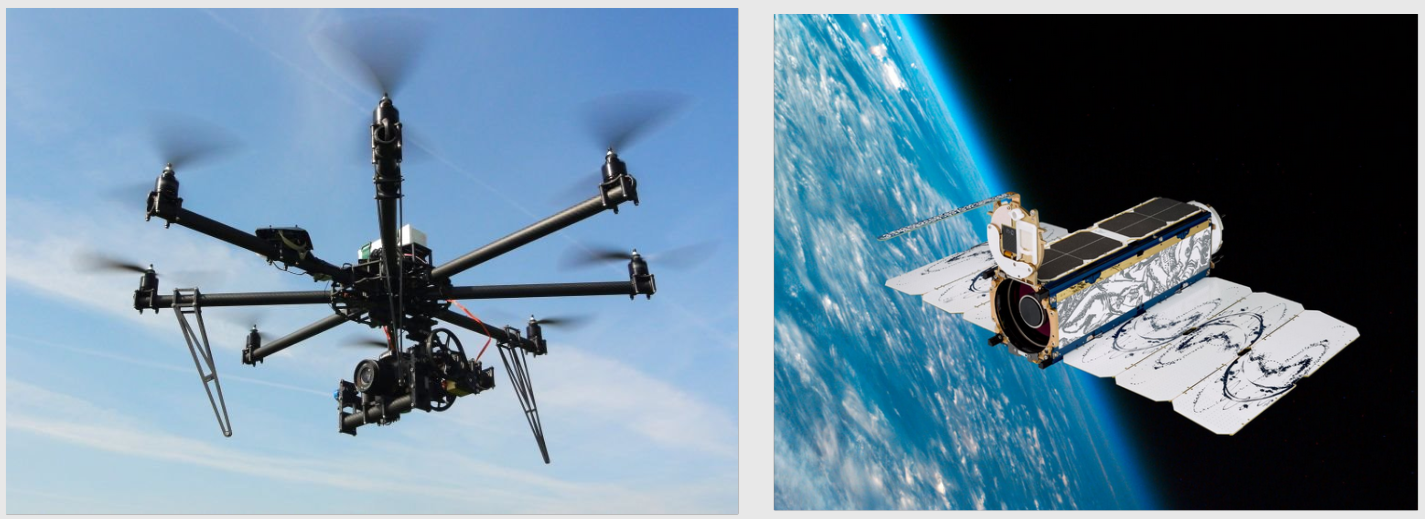
\includegraphics[height=\currprop]{figures/99_slides_only/drone_and_satellite.png}
    \end{figure}
\end{frame}

\begin{frame}{The Tool: Remote Sensing (RS)}
    \begin{block}{RS as a Key Enabler}
        In this context, Remote Sensing (RS) is a candidate tool to help accomplish this new "greener revolution".
        \begin{itemize}
            \pause
            \item It allows monitoring optimal planting and harvesting conditions.
            \pause
            \item It enables Precision Agriculture (e.g., applying chemicals locally rather than uniformly).
            \pause
            \item It allows active monitoring of deforestation.
            \pause
            \item It helps stakeholders anticipate food shortages.
        \end{itemize}
    \end{block}
\end{frame}

\begin{frame}{The Challenges}
    \begin{itemize}
        \item Expert data labeling for RS is highly expensive. Conversely, free public maps (like MapBiomas or USDA CDL) often contain noisy or inconsistent labels.
        \pause
        \item The complexity increases with the size and heterogeneity of Satellite Image Time Series (SITS).
        \pause
        \item Modern Deep Neural Networks suffer from overconfidence: they exhibit high certainty even in incorrect predictions.
    \end{itemize}
\end{frame}

\begin{frame}{The Proposed Solutions}
    \begin{itemize}
        \item Instead of just improving models, \textbf{DCAI} focuses on improving data quality. We can apply rigorous filtering to noisy public labels to create highly reliable datasets.
        \pause
        \item The amount of public RS data is massive. \textbf{SSL} extracts patterns from this unlabeled data to generate supervisory signals.
        \pause
        \item To address overconfidence, we can treat incorrect predictions as anomalies in the model's embedding space. We propose \textbf{ORDER} (Open-set Recognition for Discriminative Error Rebuttal), a post-processing strategy using Gaussian Mixture Models (GMMs) to separate correct from incorrect predictions dynamically.
    \end{itemize}
\end{frame}

\begin{frame}{Common RS Agricultural Applications}
    \renewcommand{\currprop}{0.5\textheight}
    \begin{figure}
        \centering
        \includegraphics<1| handout:0>[height=0.87\textheight]{figures/1_introduction/graphical_abstract_crop_new_fixed.pdf}
        \includegraphics<2| handout:1>[height=0.87\textheight]{figures_slides/graphical_abstract_crop_new_fixed_show.jpg}
    \end{figure}
\end{frame}

\begin{frame}{Objectives and Scope}
    \begin{block}{Objectives of This Work}
        \begin{itemize}
            \item \textbf{General Objective:} Develop and validate a reliable, lightweight, data-centric pipeline for parcel-level crop classification using SITS, capable of predicting its own failures.
            \pause
            \item \textbf{Specific Objectives:} 
            \begin{itemize}
                \item Curate public datasets using DCAI strategies.
                \item Benchmark classification architectures (from Shallow to Mamba/Transformers) and SSL techniques.
                \item Develop a confidence estimation strategy (ORDER) to rebut classification errors.
            \end{itemize}
        \end{itemize}
    \end{block}
\end{frame}

\begin{frame}{Research Questions}
    \begin{enumerate}
        \item \textbf{RQ1:} To what extent can DCAI strategies - specifically, rigorous filtering of noisy public labels (such as USDA CDL or Mapbiomas) - enable the creation of crop classification datasets and improve the performance of crop classification models?
        \item \textbf{RQ2:} Do SSL pre-training strategies impact embedding generation and offer a significant advantage over supervised models when labels are scarce? If so, which strategy generates the best embeddings?
        \item \textbf{RQ3:} Is it possible to build a lightweight pipeline that achieves satisfactory performance for crop classification that can be run without expensive hardware? If so, which models are most suitable?
    \end{enumerate}
\end{frame}

\begin{frame}{Research Questions}
    \begin{enumerate}
        \item \textbf{RQ4:} Is it possible to achieve satisfactory performance for crop classification using only public sensors?
        \item \textbf{RQ5:} Is it possible to improve confidence estimation or detect model anomalies - differ between right and wrong predictions - through generative models on embeddings, surpassing established baselines such as ConfidNet in the task of fault prediction?
    \end{enumerate}
\end{frame}
\section{Related Work}

\begin{frame}{Agricultural Remote Sensing: Sensors \& Spectral Behavior}
    \renewcommand{\currprop}{0.4\textheight}
    \begin{itemize}
    \item Remote Sensing heavily relies on capturing Electromagnetic Radiation (EMR).
    \pause
    \item Researchers use mathematical combinations of spectral bands to highlight vegetation health and age (e.g., NDVI, EVI2).
    \pause
    \item We can distinguish crop species because each plant has a unique spectral response curve 
    \end{itemize}

    \pause
    \begin{figure}
        \centering
        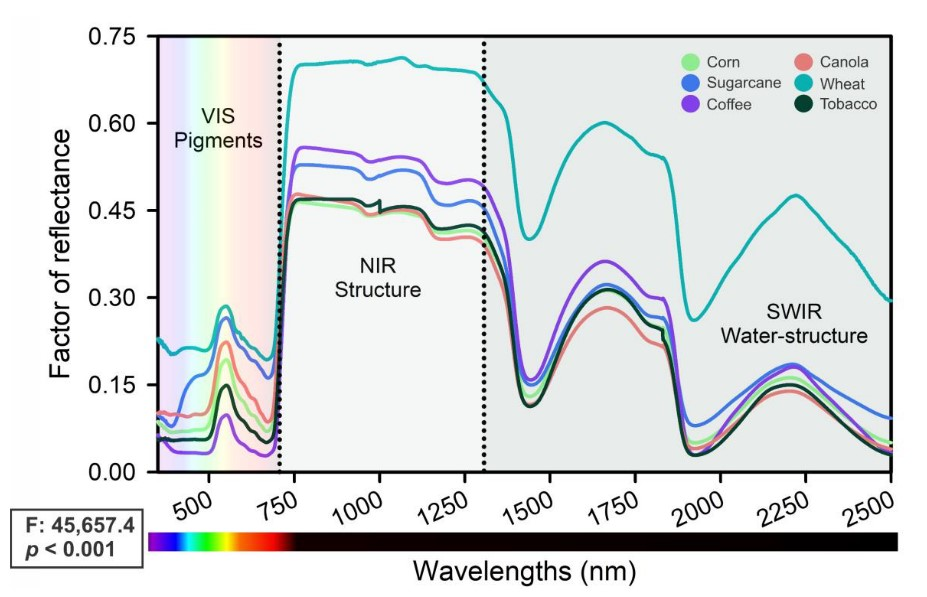
\includegraphics[height=\currprop]{figures/3_theoretical_background/veg_reflectance.jpg}
    \end{figure}
\end{frame}

\begin{frame}{Agricultural Remote Sensing: SITS \& Phenology}
    \renewcommand{\currprop}{0.5\textheight}
    \begin{block}{Satellite Image Time Series (SITS)}
        A single image is rarely enough for agriculture. SITS captures the temporal evolution of an agricultural parcel, revealing the crop's \textit{phenological cycle} (planting, growth peak, harvest).
    \end{block}
    \pause
        \begin{figure}
        \centering
        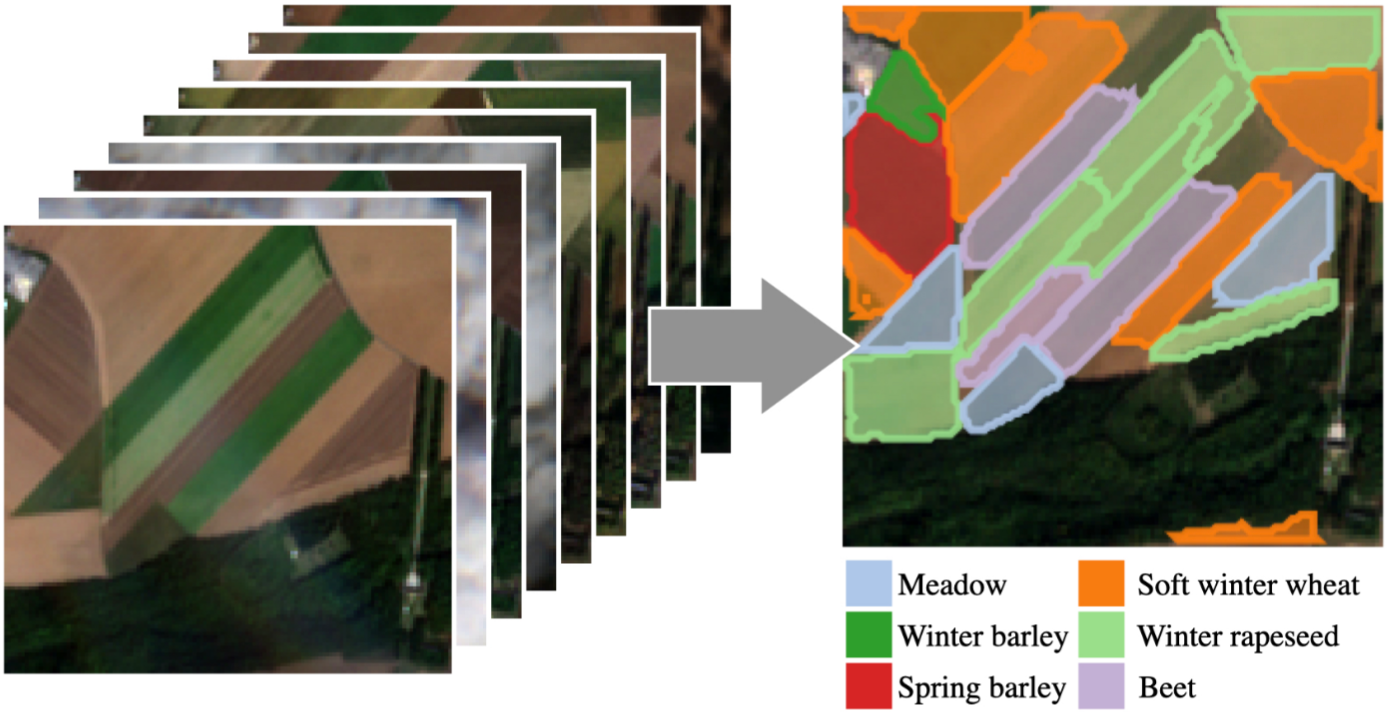
\includegraphics[height=\currprop]{figures/1_introduction/pastis-sits.png}
    \end{figure}
\end{frame}

\begin{frame}{Machine Learning: From Shallow to Deep Learning}
    \begin{block}{Shallow Learning (SL)}
        Traditional models like Random Forest (RF) and Support Vector Machines (SVM) require \textbf{Feature Engineering} (e.g., extracting monthly averages or hand-crafted indices) to process unstructured SITS data.
    \end{block}
    \pause
    \begin{block}{Deep Learning (DL)}
        Deep architectures (CNNs, LSTMs) replaced SL by learning \textbf{latent representations} directly from raw data.
        \begin{itemize}
            \item They automatically extract relevant spatial, spectral, and temporal features without manual engineering.
        \end{itemize}
    \end{block}
\end{frame}

\begin{frame}{Machine Learning: The Transformer Architecture}
    \begin{block}{Attention Mechanism}
        Originally designed for NLP\footnote[1]{\url{https://arxiv.org/abs/1706.03762}} (e.g., BERT\footnote[2]{\url{https://arxiv.org/abs/1810.04805}}), Transformers revolutionized DL processing by using \textit{self-attention} mechanisms.
        \begin{itemize}
            \item They process an entire sequence simultaneously, capturing long-range temporal dependencies better than LSTMs.
            %\item SITS-BERT is a prominent example, utilizing Positional Encoding (Day of the Year - DoY) to handle agricultural calendars.
        \end{itemize}
    \end{block}
    \pause
    \begin{block}{The Bottleneck}
        The main limitation of Transformers is their computational and memory complexity, which scales \textbf{quadratically $\mathcal{O}(L^2)$} with respect to the sequence length $L$.
    \end{block}
\end{frame}

\begin{frame}{Machine Learning: Mamba \& Post-Transformers}
    \begin{columns}[c]
        \begin{column}{0.55\textwidth}
            \begin{block}{The Post-Transformer Question}
                Can we achieve Transformer-level results without the quadratic computational cost?
            \end{block}
            
            \pause
            
            \begin{block}{The Mamba Architecture}
                Selective State Space Models\footnote[1]{\url{https://arxiv.org/abs/2312.00752}} replace quadratic attention with a hardware-aware linear selection mechanism.
                \begin{itemize}
                    \item Filter out irrelevant, focus on specific contextual data.
                    \item Operates with \textbf{linear complexity $\mathcal{O}(L)$}.
                \end{itemize}
            \end{block}
        \end{column}
        
        \begin{column}{0.40\textwidth}
            \begin{figure}
                \centering
                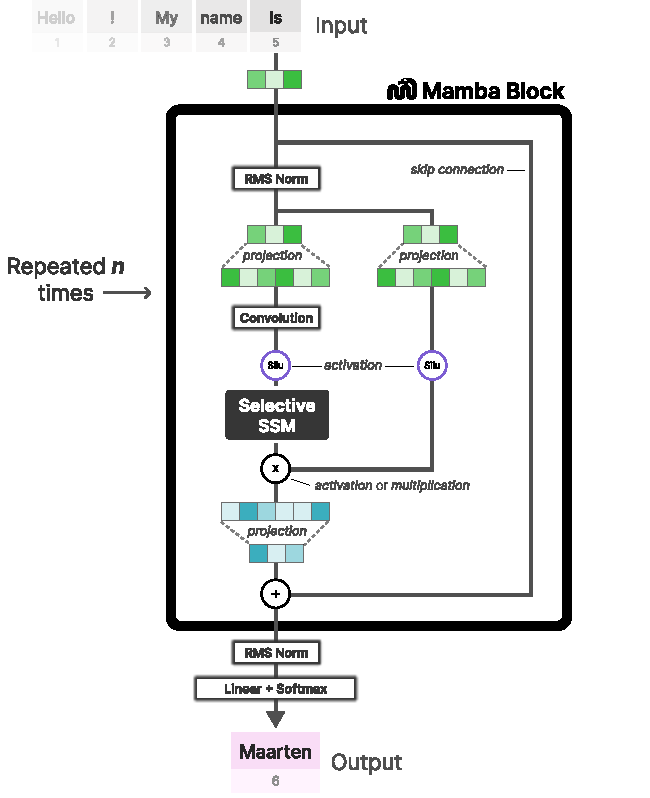
\includegraphics[width=\textwidth]{figures/3_theoretical_background/deep learning/mamba.pdf}
            \end{figure}
        \end{column}
    \end{columns}
\end{frame}
\begin{frame}{Crop Mapping: Classification of Crops}
    \begin{block}{Two Main Sub-Applications}
        \begin{itemize}
            \item \textbf{Post-harvest classification:} Uses the complete time series (more common and simpler).
                \pause
                \begin{itemize}
                    \item \textbf{CNNs} remain highly used (e.g., 3D CNN, CNNs with Attention).
                    \item \textbf{MIM/Generative SSL} (SITS-BERT, SITS-Former) and \textbf{Contrastive SSL} (SITS-MoCo) strategies on Transformers achieve SOTA results by reconstructing masked time series.
                \end{itemize}
            \pause
            \item \textbf{In-season classification:} Produces results \textbf{before} harvest (more complex, economically desirable).
                \pause
                \begin{itemize}
                    \item Focus on \textbf{early recognition} using CNNs and recurrent models (e.g., ConvLSTM, 3D CNN over time).
                    \item Specialized techniques like an \textbf{Earliness-Rewarded Loss} are used to train models for early prediction.
                \end{itemize}
        \end{itemize}
    \end{block}
\end{frame}

\section{Data Acquisition, SITS Datasets and Preprocessing}

\begin{frame}{Data Sources: Varda Global FieldID}
\begin{block}{Parcel Geometries}
A collaborative database providing spatial delineations of agricultural plots worldwide.
\end{block}
%\pause
\begin{figure}
\centering
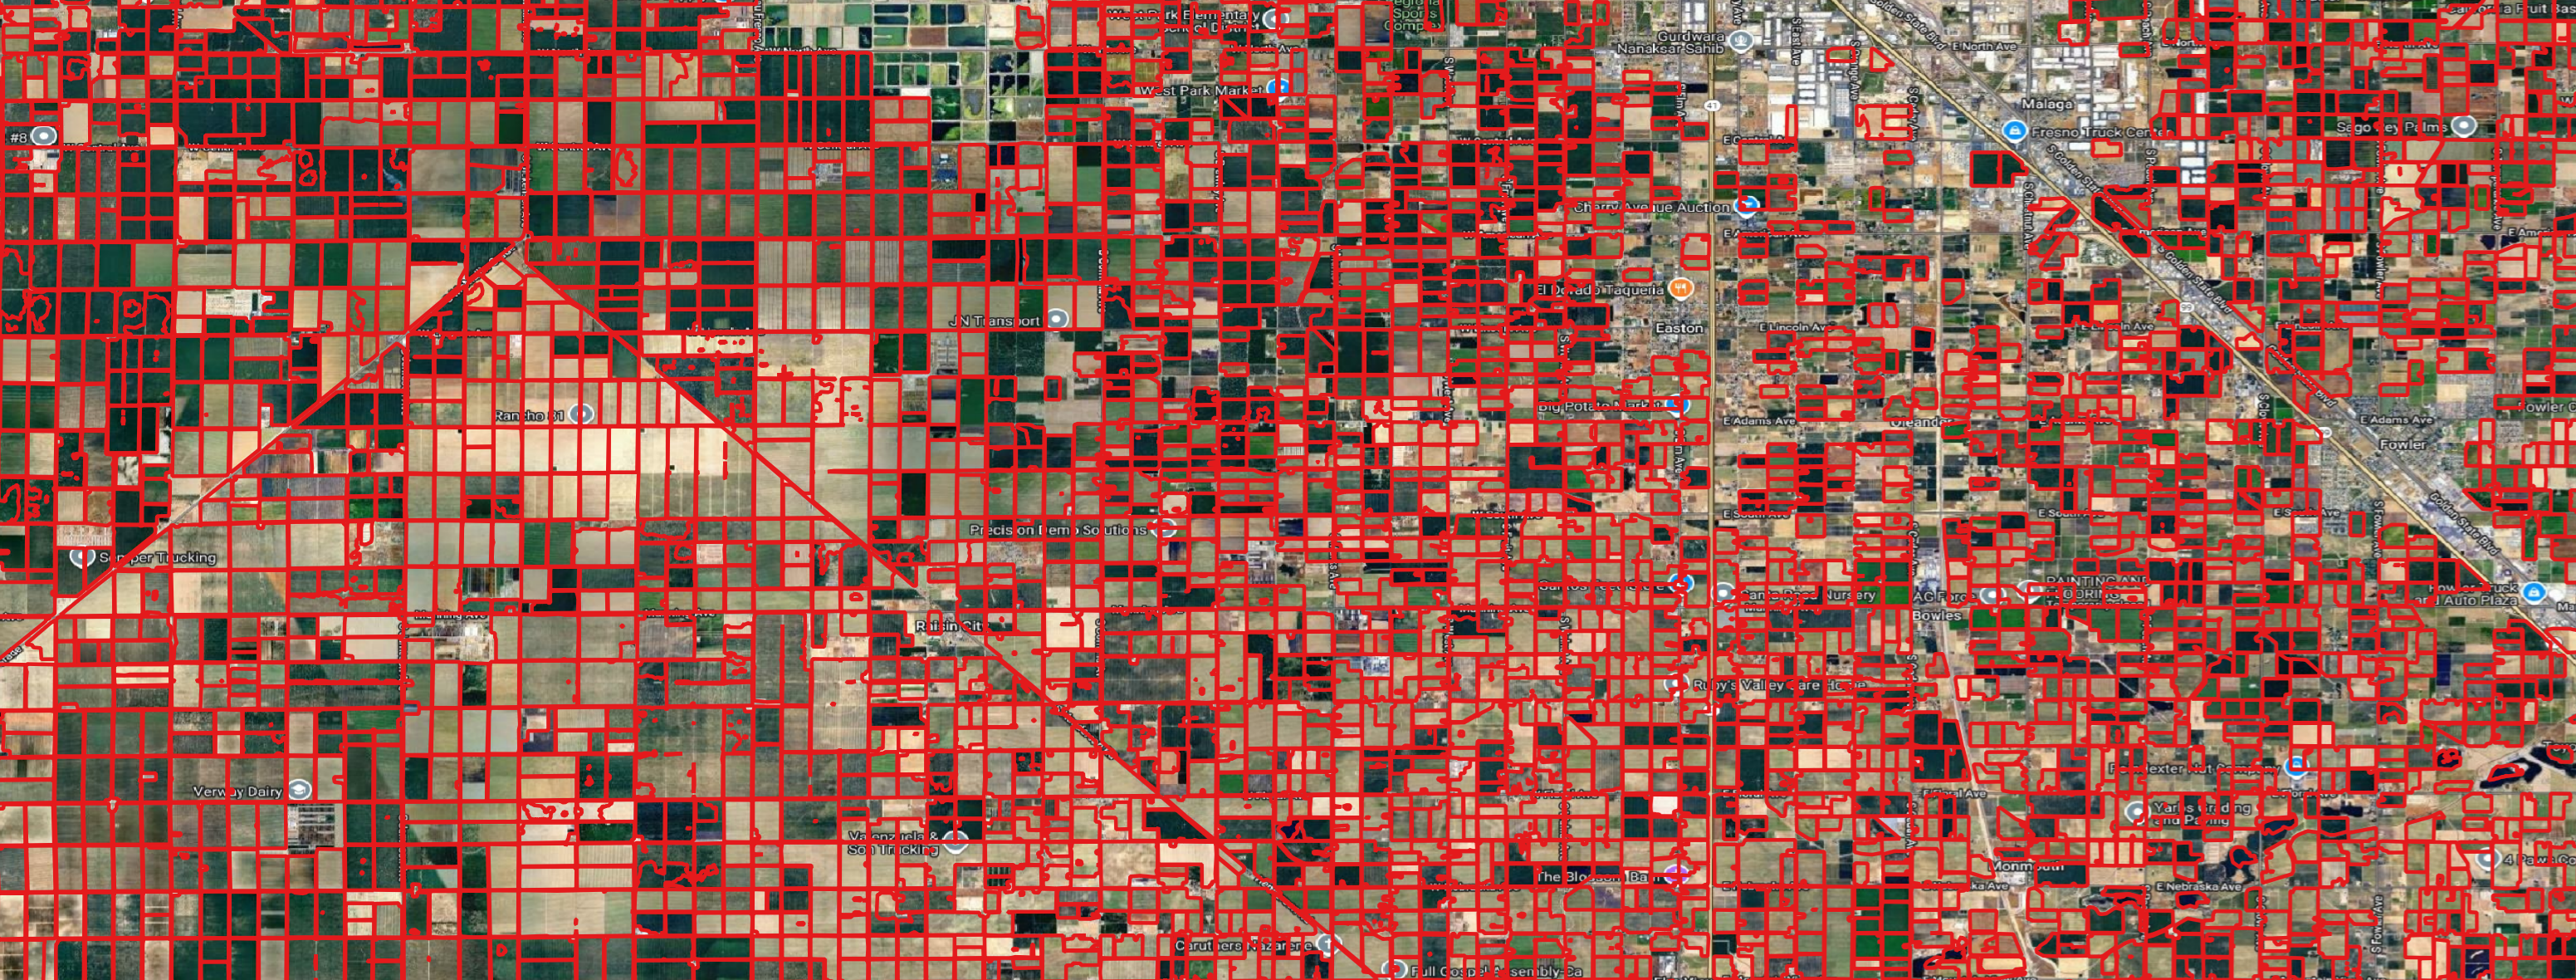
\includegraphics[width=\textwidth]{figures/6_methodology/varda/varda_fresno.png} 
\caption*{Well-delineated parcels in Fresno, California.}
\end{figure}
\end{frame}

\begin{frame}{Data Sources: Varda Global FieldID}
\renewcommand{\currprop}{1\textheight}
\begin{block}{The Challenge}
Public data contains noise, such as parcels mistakenly identified in water bodies, requiring strict filtering.
\end{block}
%\pause
\begin{figure}
\centering
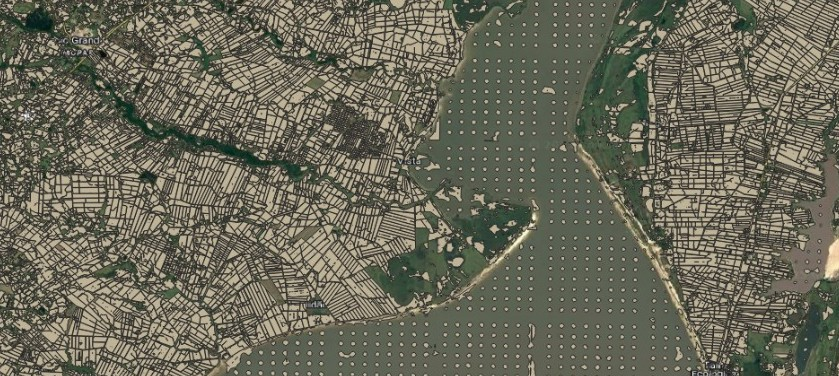
\includegraphics[width=0.9\textwidth]{figures_slides/varda_erros_slide.jpg}
\caption*{Mistakenly identified plots in water of Lagoa dos Patos.}
\end{figure}
\end{frame}

\begin{frame}{Data Sources: MapBiomas Brazil}
    \begin{columns}[c]
        \begin{column}{0.5\textwidth}
            \begin{block}{Brazilian Labels}
                Annual Land Use and Land Cover maps covering the historical series from 1985 to the present (30m resolution).
            \end{block}
            %\pause
            \begin{block}{Agricultural Theme}
                Subdivides into temporary and perennial crops (e.g., Soybean, Sugar Cane, Pasture, Coffee, Citrus).
            \end{block}
        \end{column}
        \begin{column}{0.5\textwidth}
            \begin{figure}
                \centering
                % Figura 40 da dissertação
                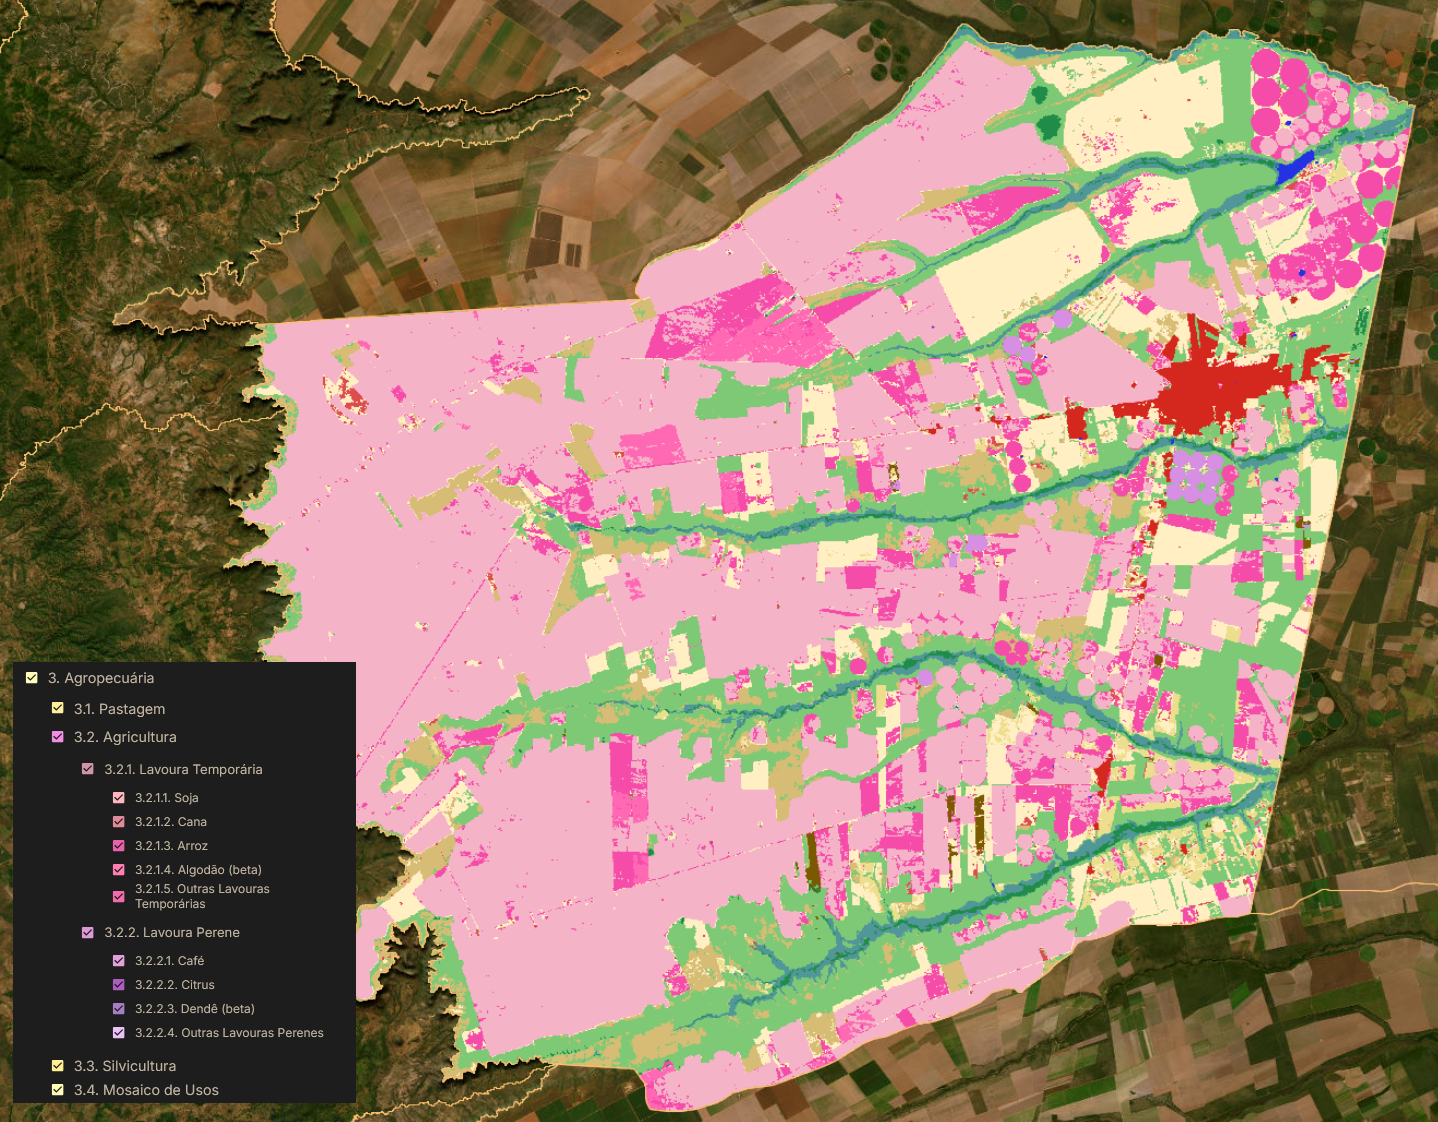
\includegraphics[width=0.9\textwidth]{figures/6_methodology/mapbiomas.png} 
                \caption*{MapBiomas Cropland Raster}
            \end{figure}
        \end{column}
    \end{columns}
\end{frame}

\begin{frame}{Data Sources: USDA Cropland Data Layer (CDL)}
    \begin{columns}[c]
        \begin{column}{0.5\textwidth}
            \begin{block}{USA Labels}
                High-resolution specific agricultural crop masks provided by the National Agricultural Statistics Service (NASS).
            \end{block}
            %\pause
            \begin{block}{Coverage}
                Used to extract specific crop labels for the Texas and California datasets (e.g., Corn, Cotton, Almonds).
            \end{block}
        \end{column}
        \begin{column}{0.5\textwidth}
            \begin{figure}
                \centering
                % Figura 41 da dissertação
                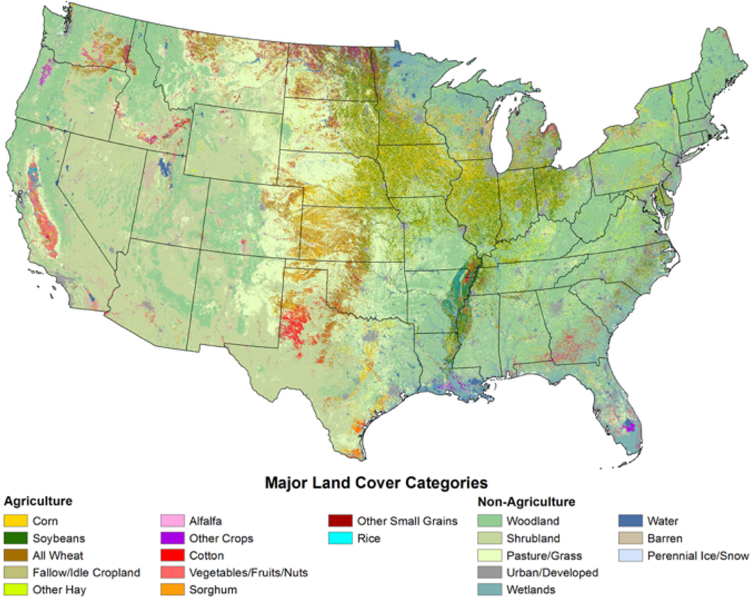
\includegraphics[width=0.9\textwidth]{figures/6_methodology/USDA.png} 
                \caption*{USDA CDL Raster}
            \end{figure}
        \end{column}
    \end{columns}
\end{frame}


\begin{frame}{Lightweight SITS Download Strategy}
    \renewcommand{\currprop}{0.6\textheight}
    
    \begin{block}{Acquiring high confidence labels and features}
    \only<1| handout:0>{We initiate the pipeline by matching raw cropland rasters with precise parcel delineations}%
    \only<2| handout:0>{This data is processed within GEE Cloud (using our library) to extract comprehensive vegetation indices.}%
    \only<3| handout:0>{A vegetative filter basead on thresholds ensures the acquisition of highly reliable, high-confidence crop labels.}%
    \only<4| handout:0>{The result are high confidence parcel crop classification labels.}%
    \only<5| handout:0>{To explain the SITS download, let's take a look at a single sample.}%
    \only<6| handout:0>{Raw satellite images are selected if they intersect with the parcel geometry.}%
    \only<7| handout:0>{All images are cropped by the parcel geometry.}%
    \only<8| handout:0>{Clouds and cloud shadows pixels are filtered out in each image.}%
    \only<9| handout:0>{The clear pixels are then spatially aggregated to generate clear statistical metrics, such median.}%
    \only<10| handout:1>{The final result of the download strategy are treated resulting SITS and crop classes.}%
\end{block}
\begin{figure}
    \centering
    \includegraphics<1| handout:0>[height=\currprop]{figures_slides/datasets_8.jpg}%
    \includegraphics<2| handout:0>[height=\currprop]{figures_slides/datasets_7.jpg}%
    \includegraphics<3| handout:0>[height=\currprop]{figures_slides/datasets_6.jpg}%
    \includegraphics<4| handout:0>[height=\currprop]{figures_slides/datasets_5.jpg}%
    \includegraphics<5| handout:0>[height=\currprop]{figures_slides/datasets_4.jpg}%
    \includegraphics<6| handout:0>[height=\currprop]{figures_slides/datasets_3.jpg}%
    \includegraphics<7| handout:0>[height=\currprop]{figures_slides/datasets_2.jpg}%
    \includegraphics<8| handout:0>[height=\currprop]{figures_slides/datasets_1.jpg}%
    \includegraphics<9| handout:0>[height=\currprop]{figures_slides/datasets_0.jpg}%
    \includegraphics<10| handout:1>[height=\currprop]{figures_slides/datasets_final.jpg}%
\end{figure}
\end{frame}
\begin{frame}{The Proposed SITS Datasets}
    \begin{block}{Three Novel Parcel-Level Datasets}
        We generated three datasets: \textbf{Texas} (7 classes), \textbf{California} (14 classes), and \textbf{Brazil} (10 classes).
    \end{block}
    \pause
    \begin{block}{The Complexity of the Brazilian Dataset}
        Unlike the US regions (mostly single-cycle monocultures), Brazil presents unique challenges:
        \begin{itemize}
            \item \textbf{Subcontinental scale:} High regional variability in planting schedules across different biomes.
            \item \textbf{Double/Triple Cropping ("Safrinha"):} The presence of secondary crops acts as spectral noise, since public maps (like MapBiomas) provide only the primary crop label.
            \item \textbf{Noise from crop source:} MapBiomas deals with land use and cover, not active agriculture. 
        \end{itemize}
    \end{block}
\end{frame}

%%%%%%%%%%%%%%%%%%%%%%%%%%%%%%%%%%%%%%%%%%%%%%%%%%%%%%%%%%%%%%%%%%%%%%%%%%

\begin{frame}{Dataset Characteristics: Class Imbalance}
    \vspace{0.2cm}
    
    \begin{columns}[c]
        \begin{column}{0.33\textwidth}
            \begin{figure}
                \centering
                % Figura 44 da dissertação
                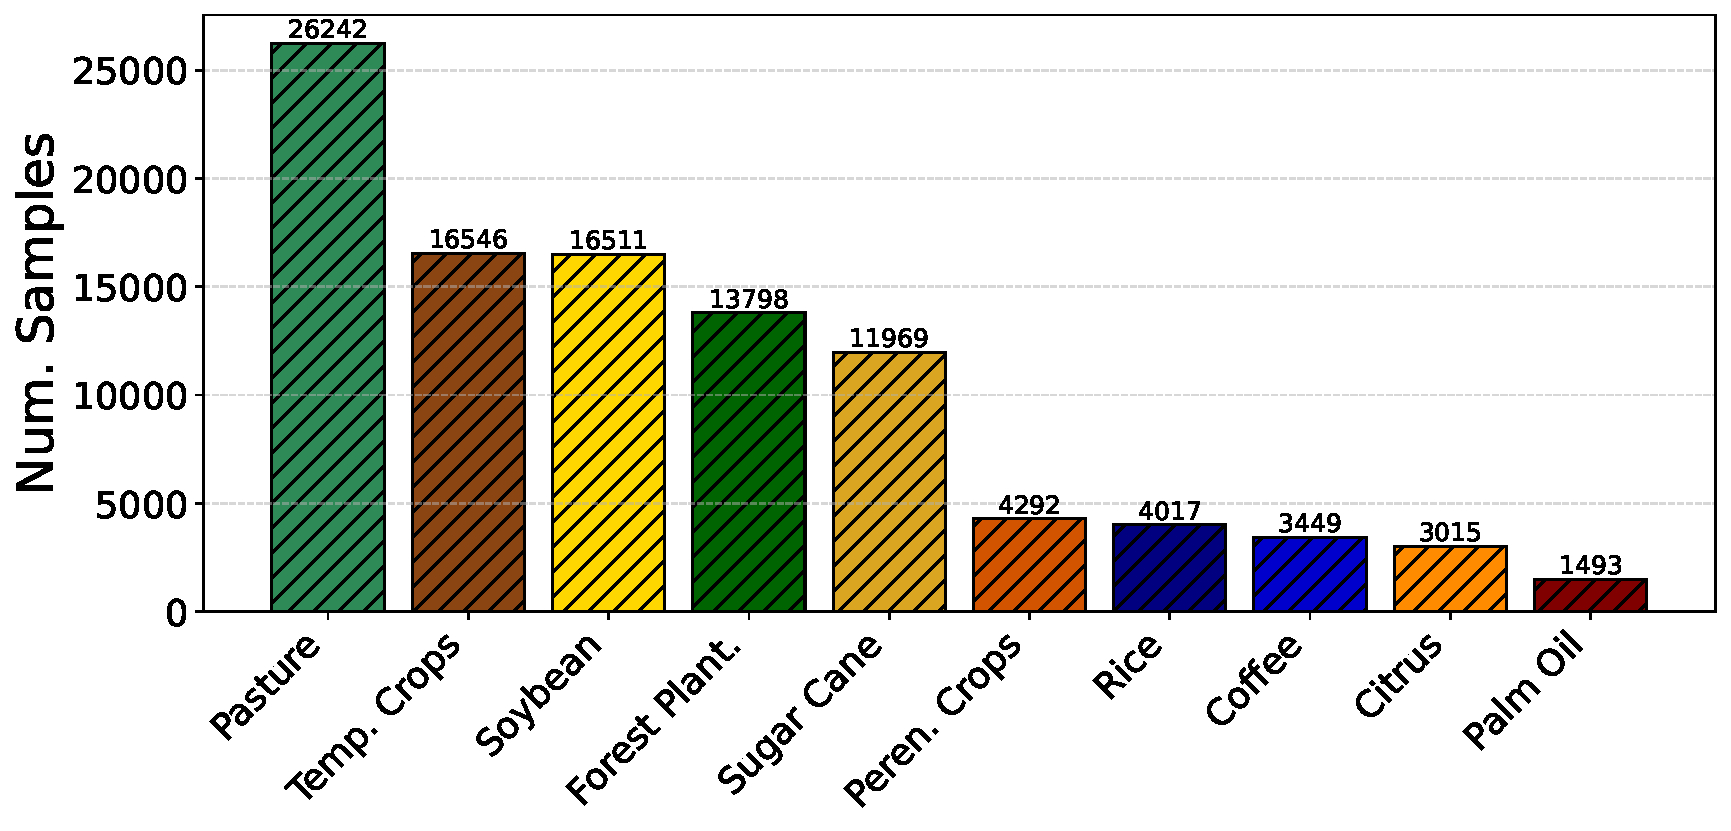
\includegraphics[width=\textwidth]{figures/6_methodology/datasets/brazil_bar_crop.pdf} 
                \caption*{Brazil (10 classes)}
            \end{figure}
        \end{column}
        \begin{column}{0.33\textwidth}
            \begin{figure}
                \centering
                % Figura 45 da dissertação
                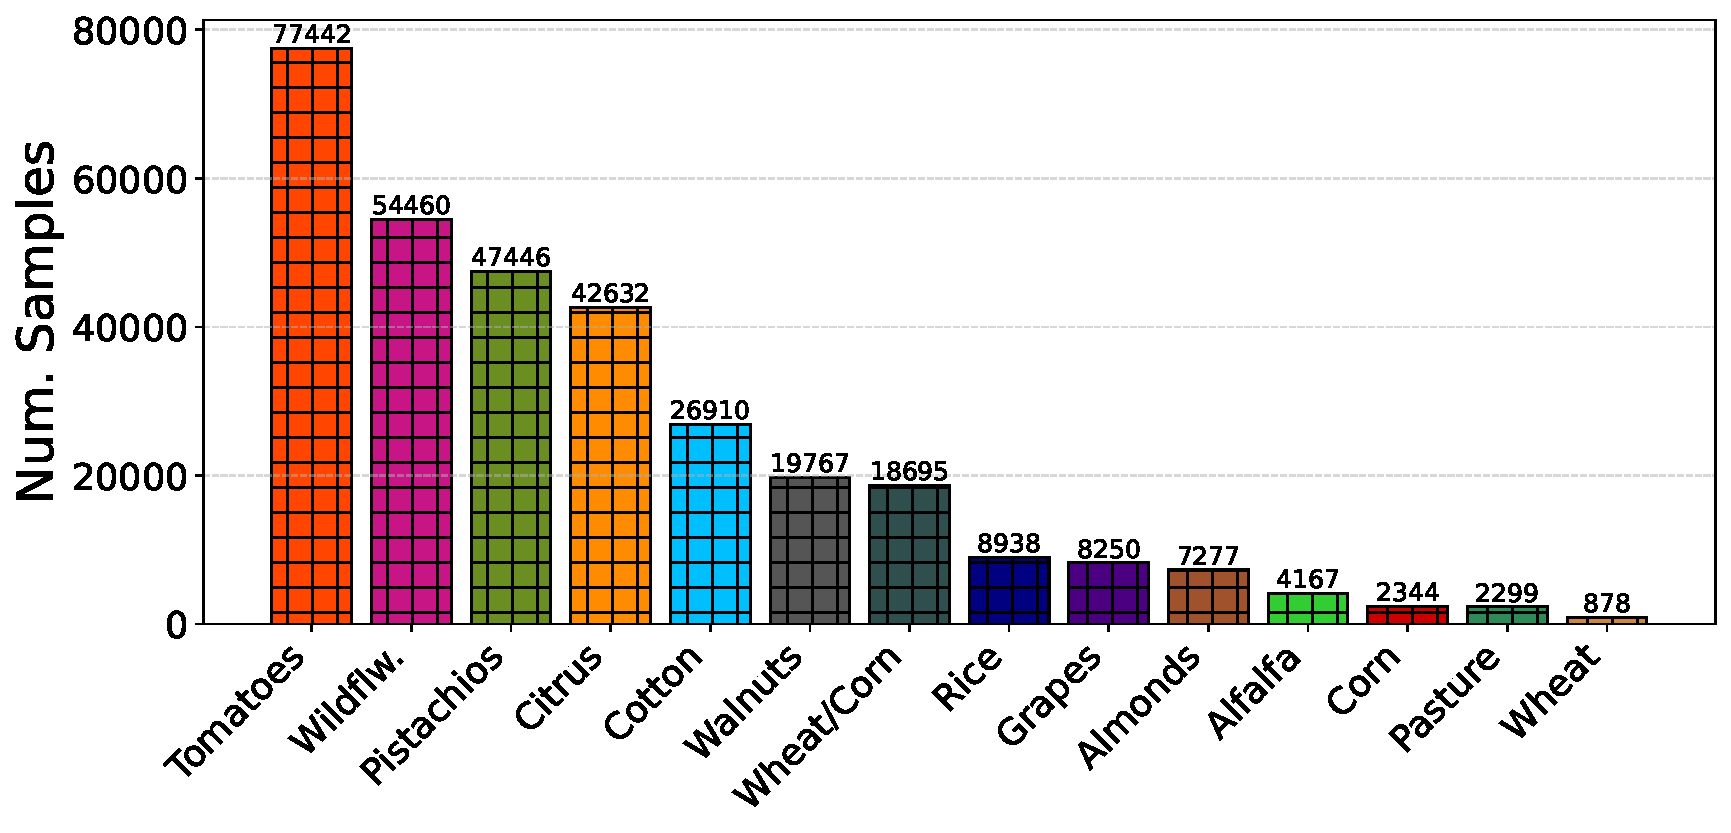
\includegraphics[width=\textwidth]{figures/6_methodology/datasets/california_bar_crop.pdf} 
                \caption*{California (14 classes)}
            \end{figure}
        \end{column}
        \begin{column}{0.33\textwidth}
            \begin{figure}
                \centering
                % Figura 46 da dissertação
                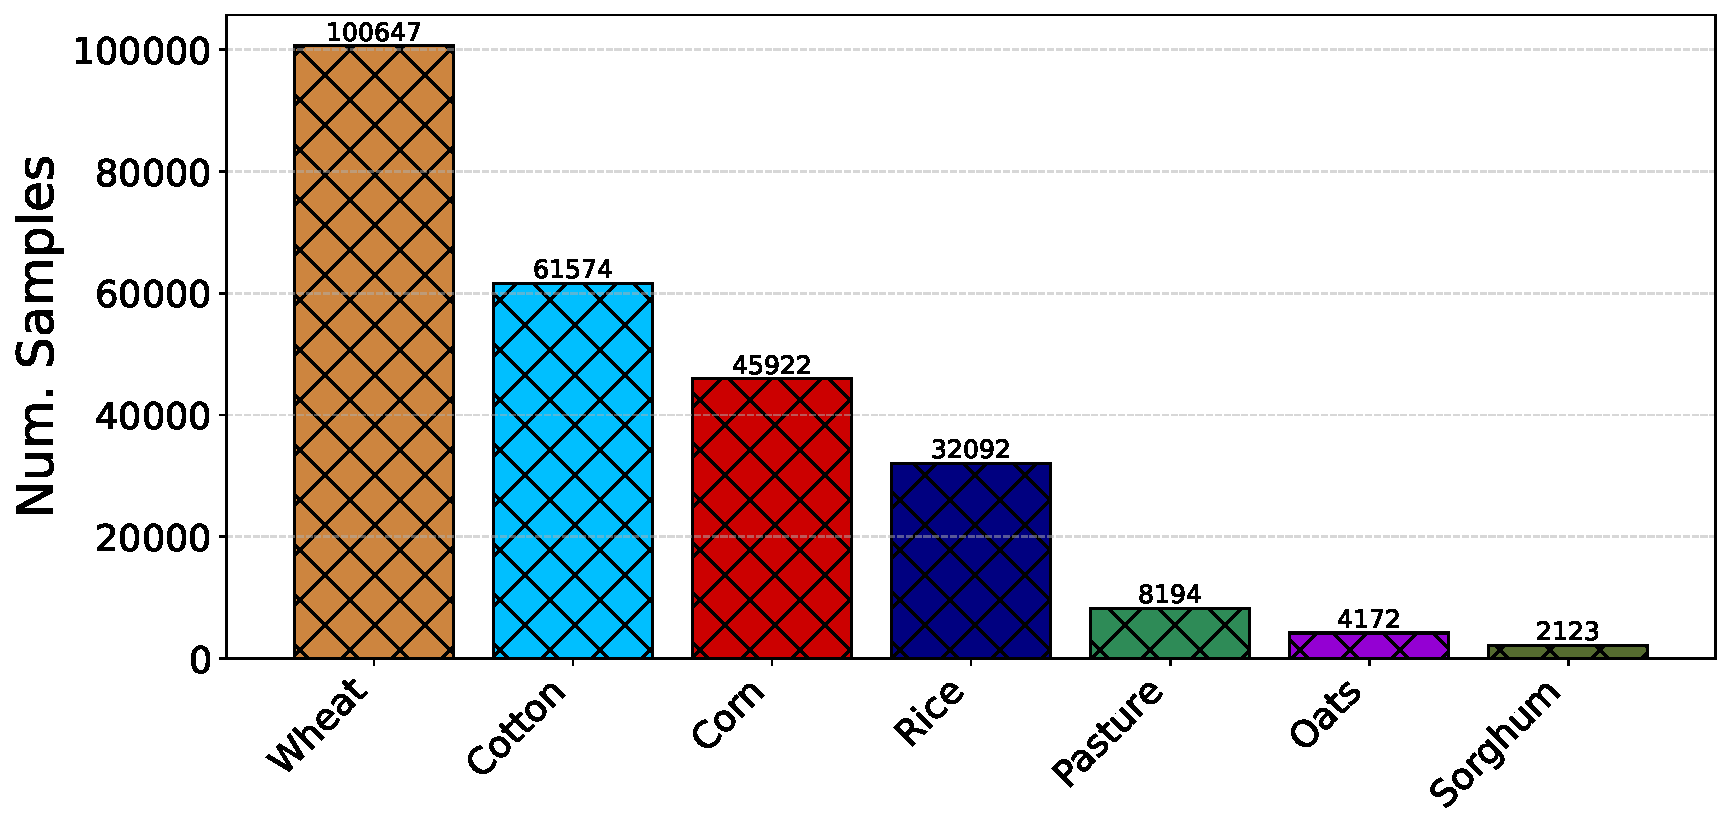
\includegraphics[width=\textwidth]{figures/6_methodology/datasets/texas_bar_crop.pdf} 
                \caption*{Texas (7 classes)}
            \end{figure}
        \end{column}
    \end{columns}
\end{frame}

\begin{frame}{Brazil Dataset Geospatial Distribution}
    \begin{figure}
        \centering
        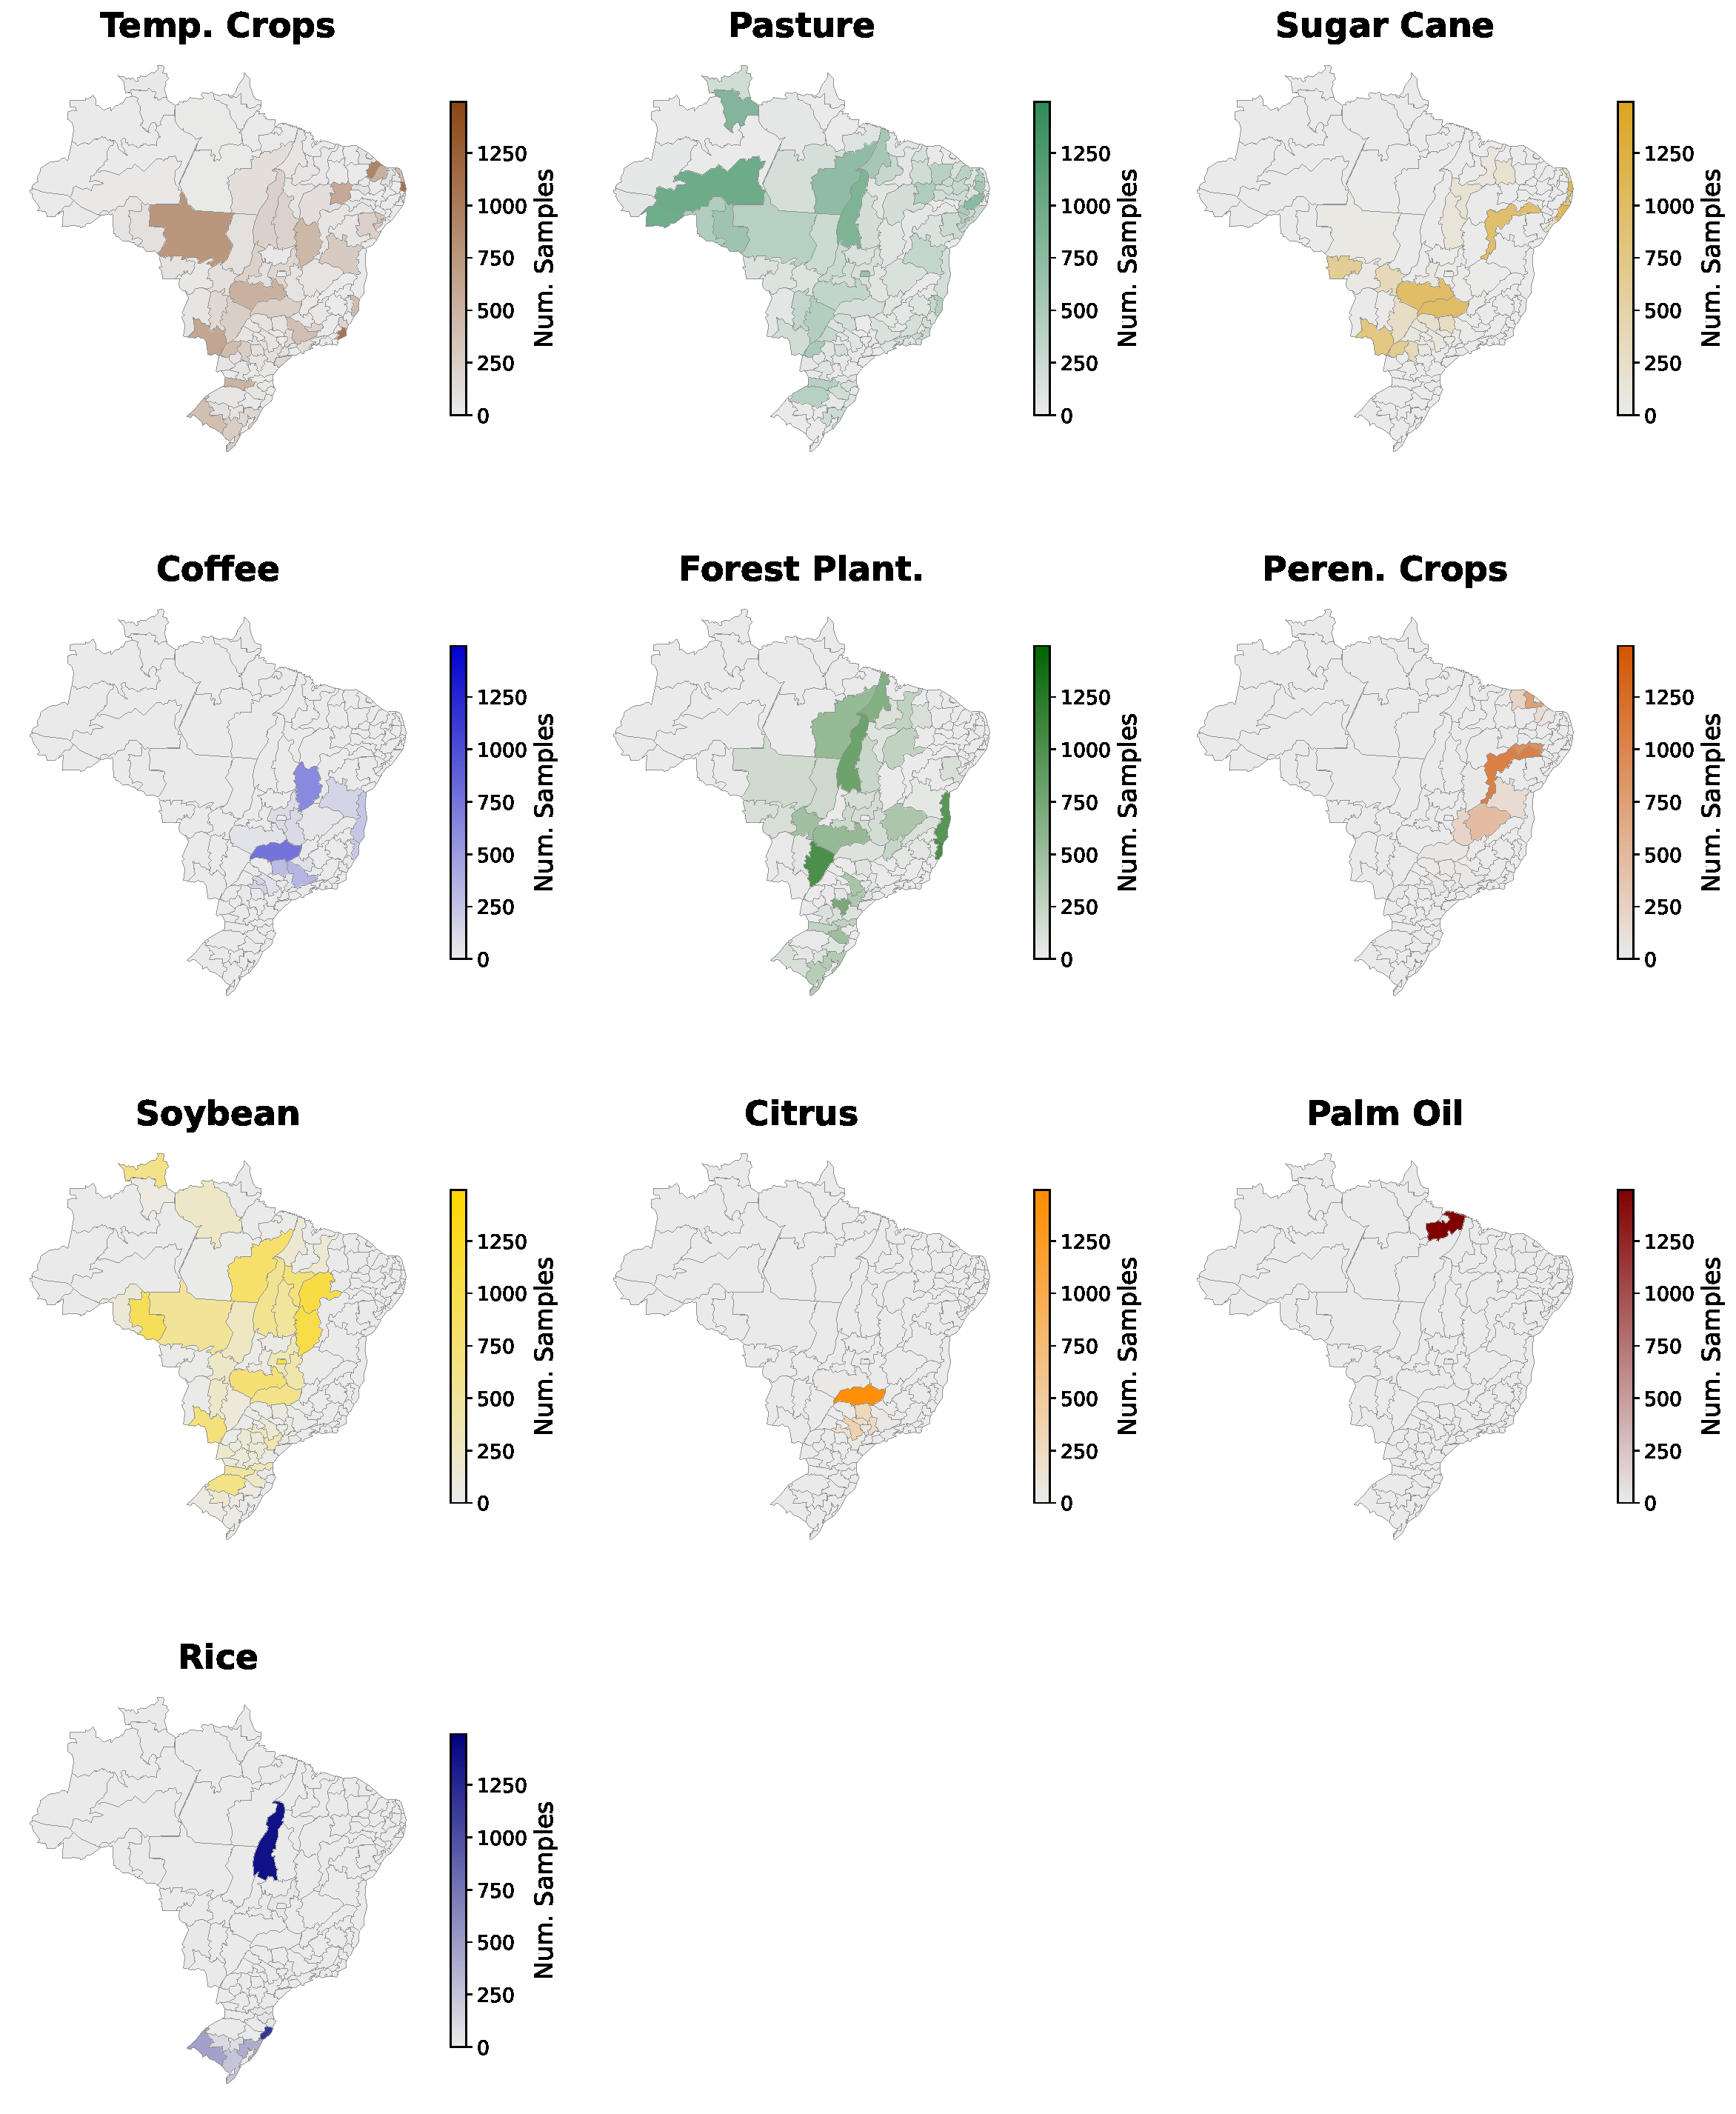
\includegraphics[width=0.7\textwidth]{figures/6_methodology/datasets/brazil_map_crops.pdf}
    \end{figure}
\end{frame}

% --- EVI2 SIGNATURES ---

\begin{frame}{Phenological Signatures (EVI2): Brazil Dataset}
    \begin{block}{The ``Safrinha'' Challenge}
        \begin{itemize}
            \item \textbf{Double Cropping \& Label Noise:} Temporary crops (e.g., Soybean) show secondary peaks. MapBiomas maps only the primary crop, adding spectral noise.
            \item \textbf{Perennials:} Classes like Forest Plantation exhibit stable, high EVI2 values year-round.
        \end{itemize}
    \end{block}
    
    \begin{figure}
        \centering
        % Figura 48 da dissertação
        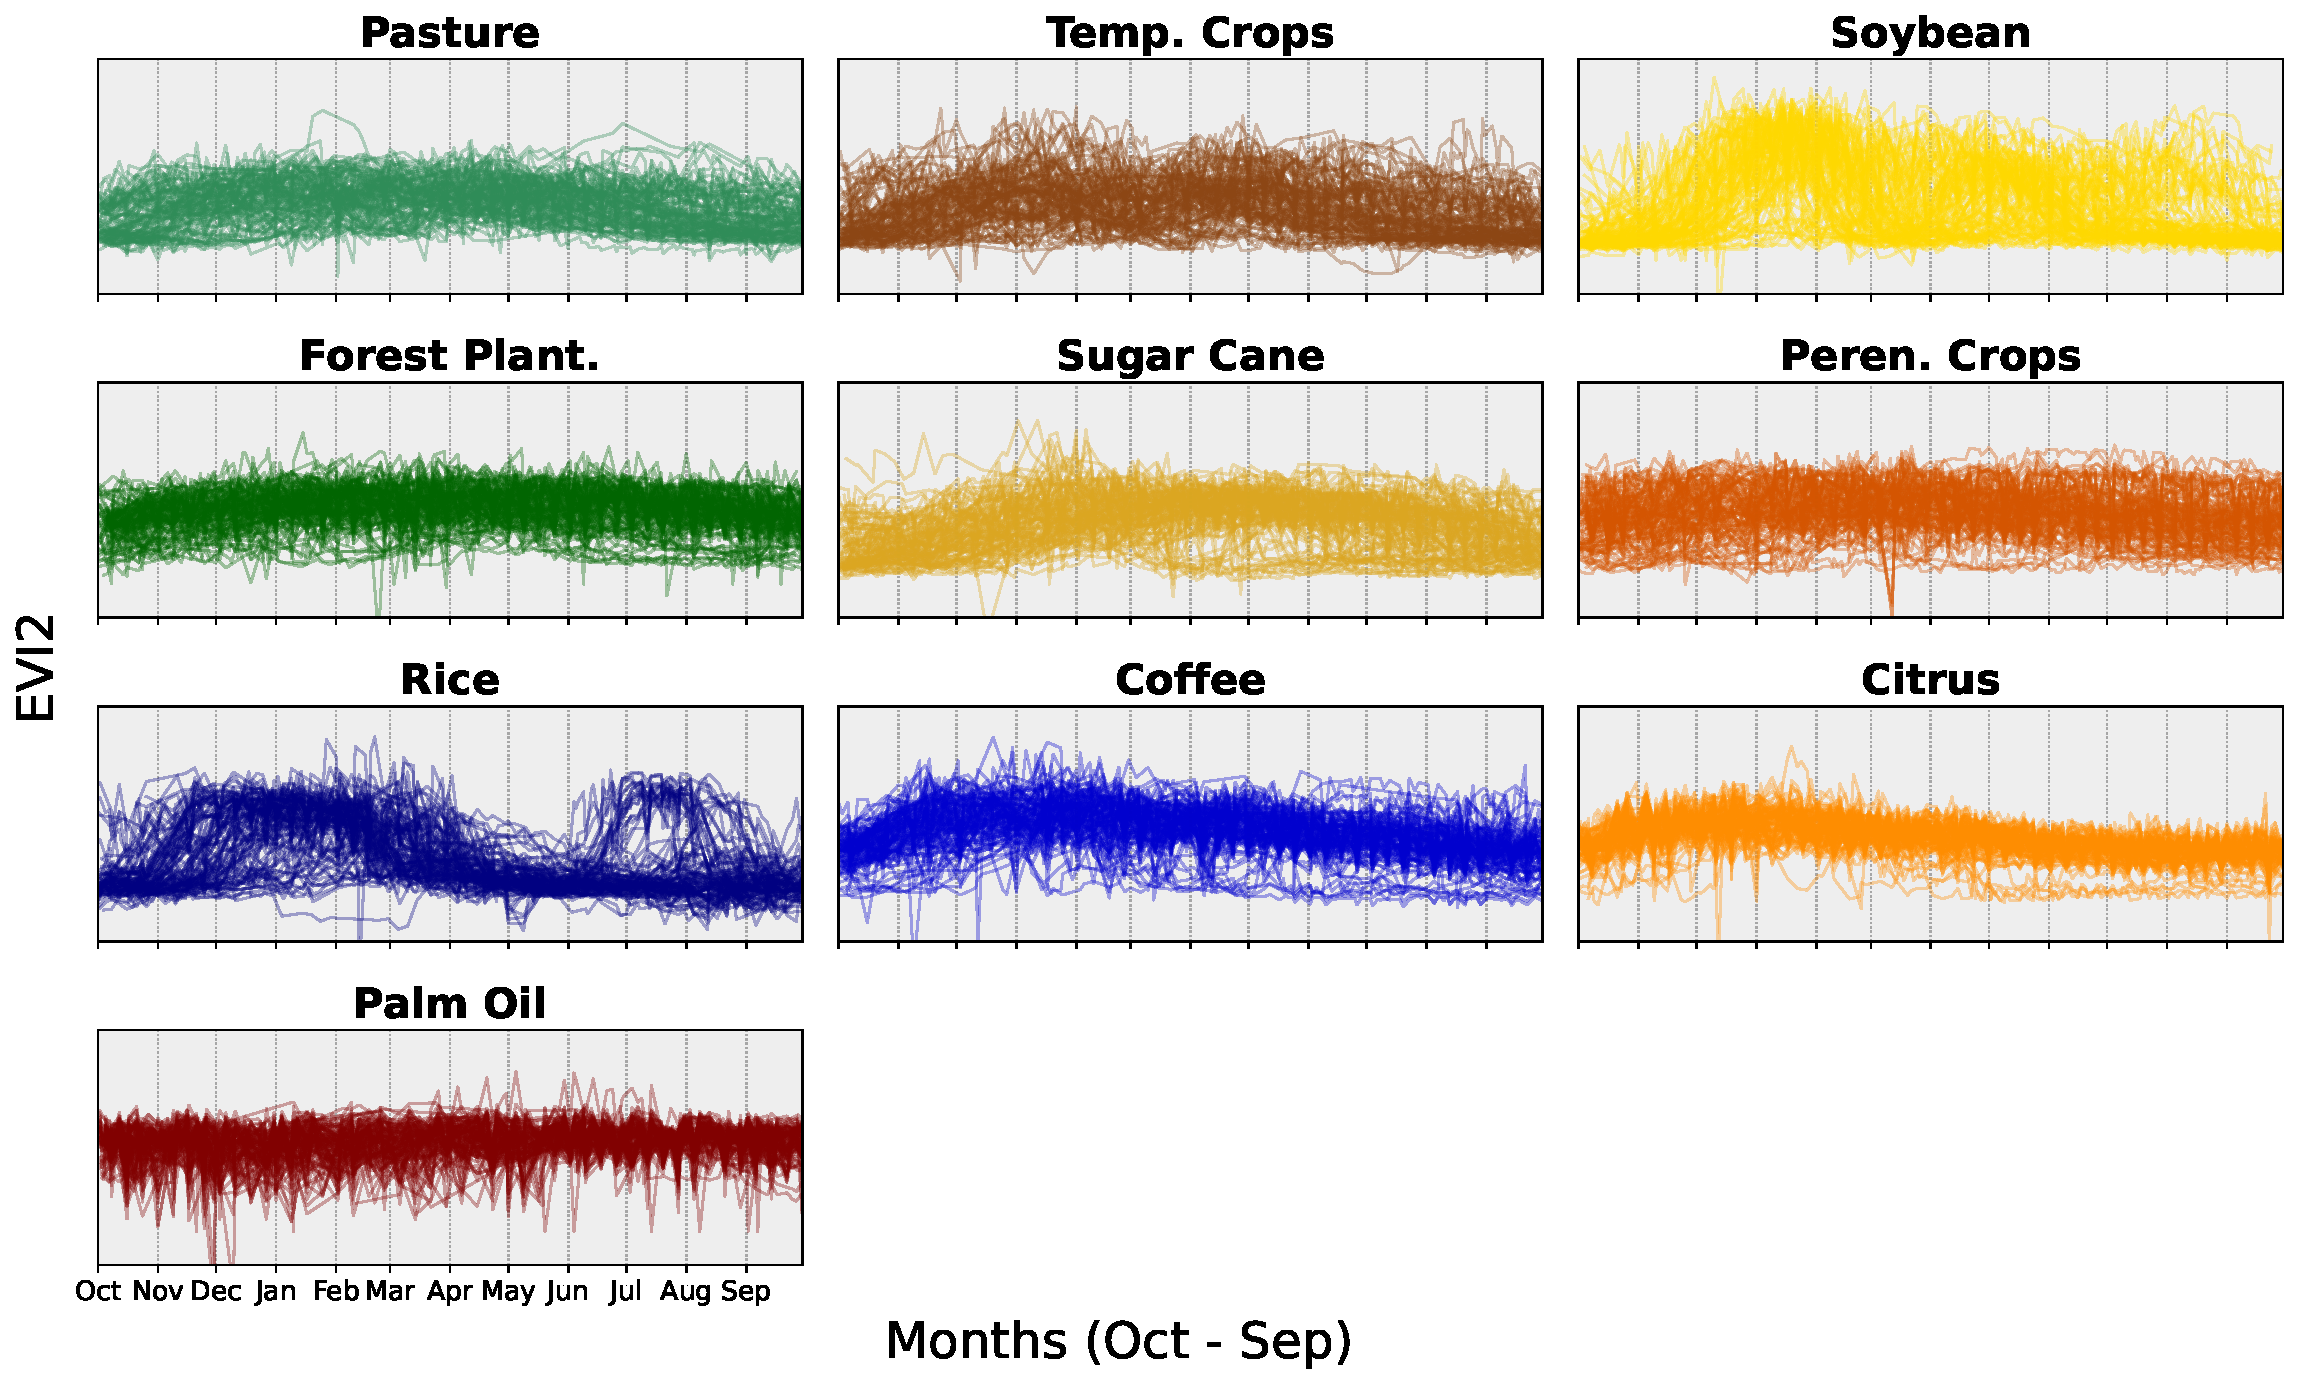
\includegraphics[height=0.4\textheight, width=\textwidth, keepaspectratio]{figures/6_methodology/datasets/brazil_evi2.pdf} 
    \end{figure}
\end{frame}

\begin{frame}{Phenological Signatures (EVI2): California Dataset}
    \begin{block}{Crop Signatures in California}
        \begin{itemize}
            \item \textbf{Clearer Signatures:} More pronounced behaviors and less label noise than Brazil.
            \item \textbf{Single-cycle:} Predominantly single-cycle crops.
            \item \textbf{Rotation:} A specific labeled class (\textit{Wheat/Corn}) exhibits a distinct double-peak signature.
        \end{itemize}
    \end{block}
    
    \begin{figure}
        \centering
        % Figura 49 da dissertação
        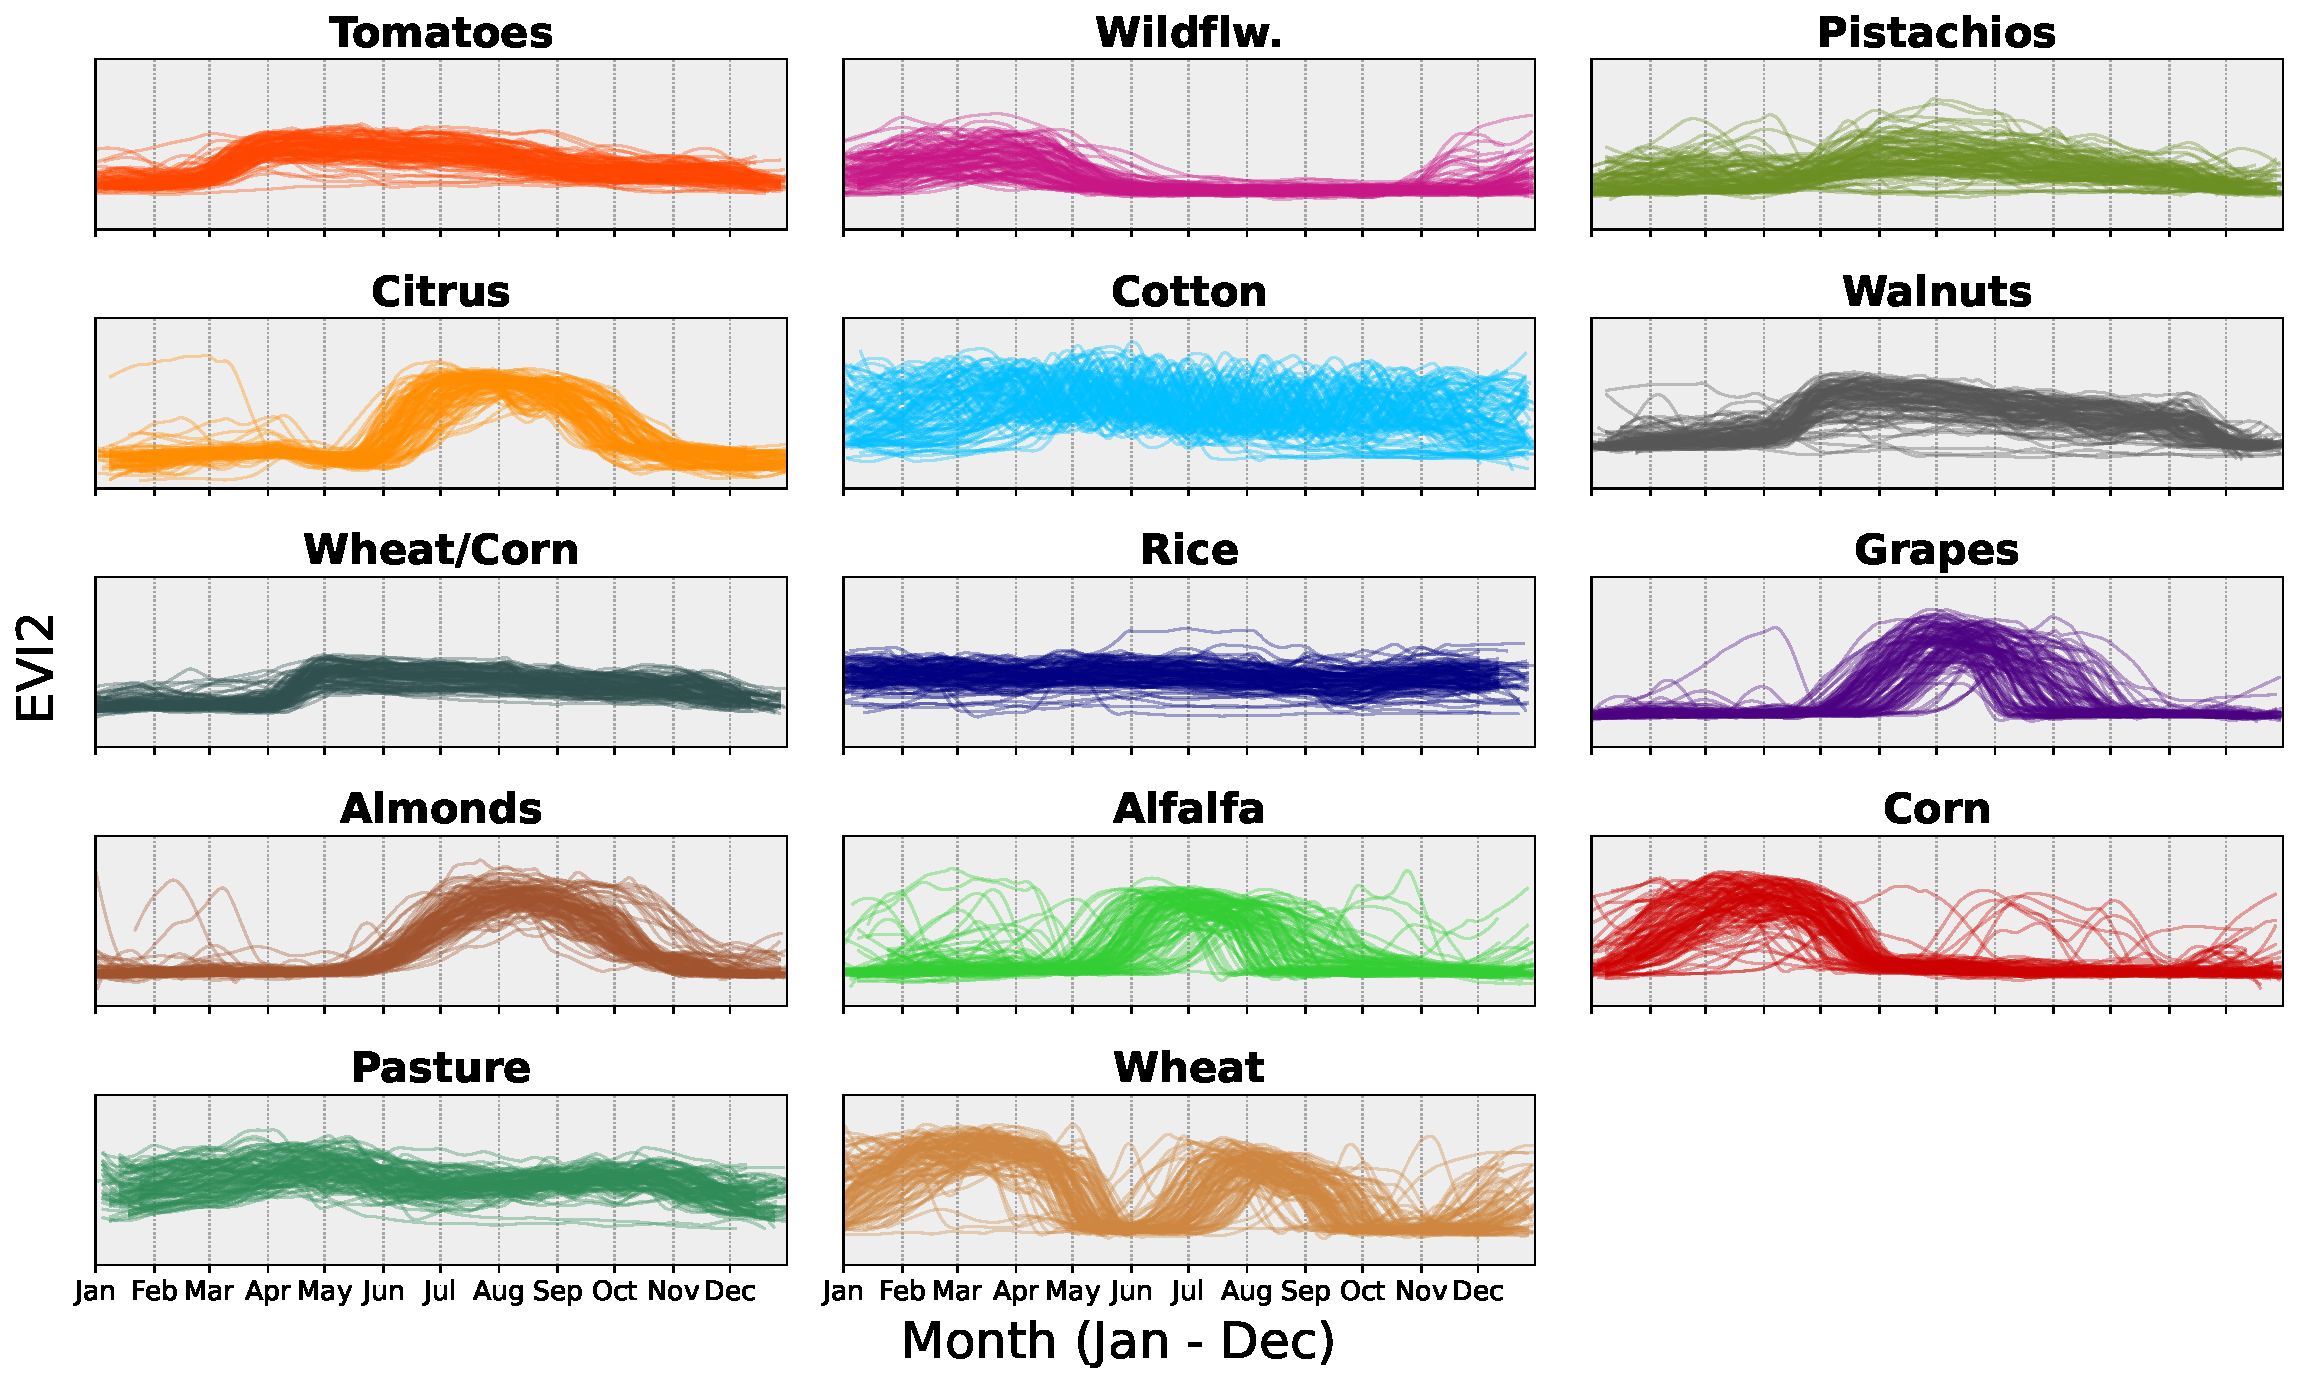
\includegraphics[height=0.4\textheight, width=\textwidth, keepaspectratio]{figures/6_methodology/datasets/california_evi2.pdf} 
    \end{figure}
\end{frame}

\begin{frame}{Phenological Signatures (EVI2): Texas Dataset}
    \begin{block}{Crop Signatures in Texas}
        \begin{itemize}
            \item \textbf{Clearest Separation:} The clearest spectral separation among all regions evaluated.
            \item \textbf{Monocultures:} Dominated by single-cycle crops with clear, single-peak curves (e.g., Cotton, Corn).
            \item \textbf{Fallow Periods:} Long, well-defined fallow periods ease the classification task.
        \end{itemize}
    \end{block}
    
    \begin{figure}
        \centering
        % Figura 50 da dissertação
        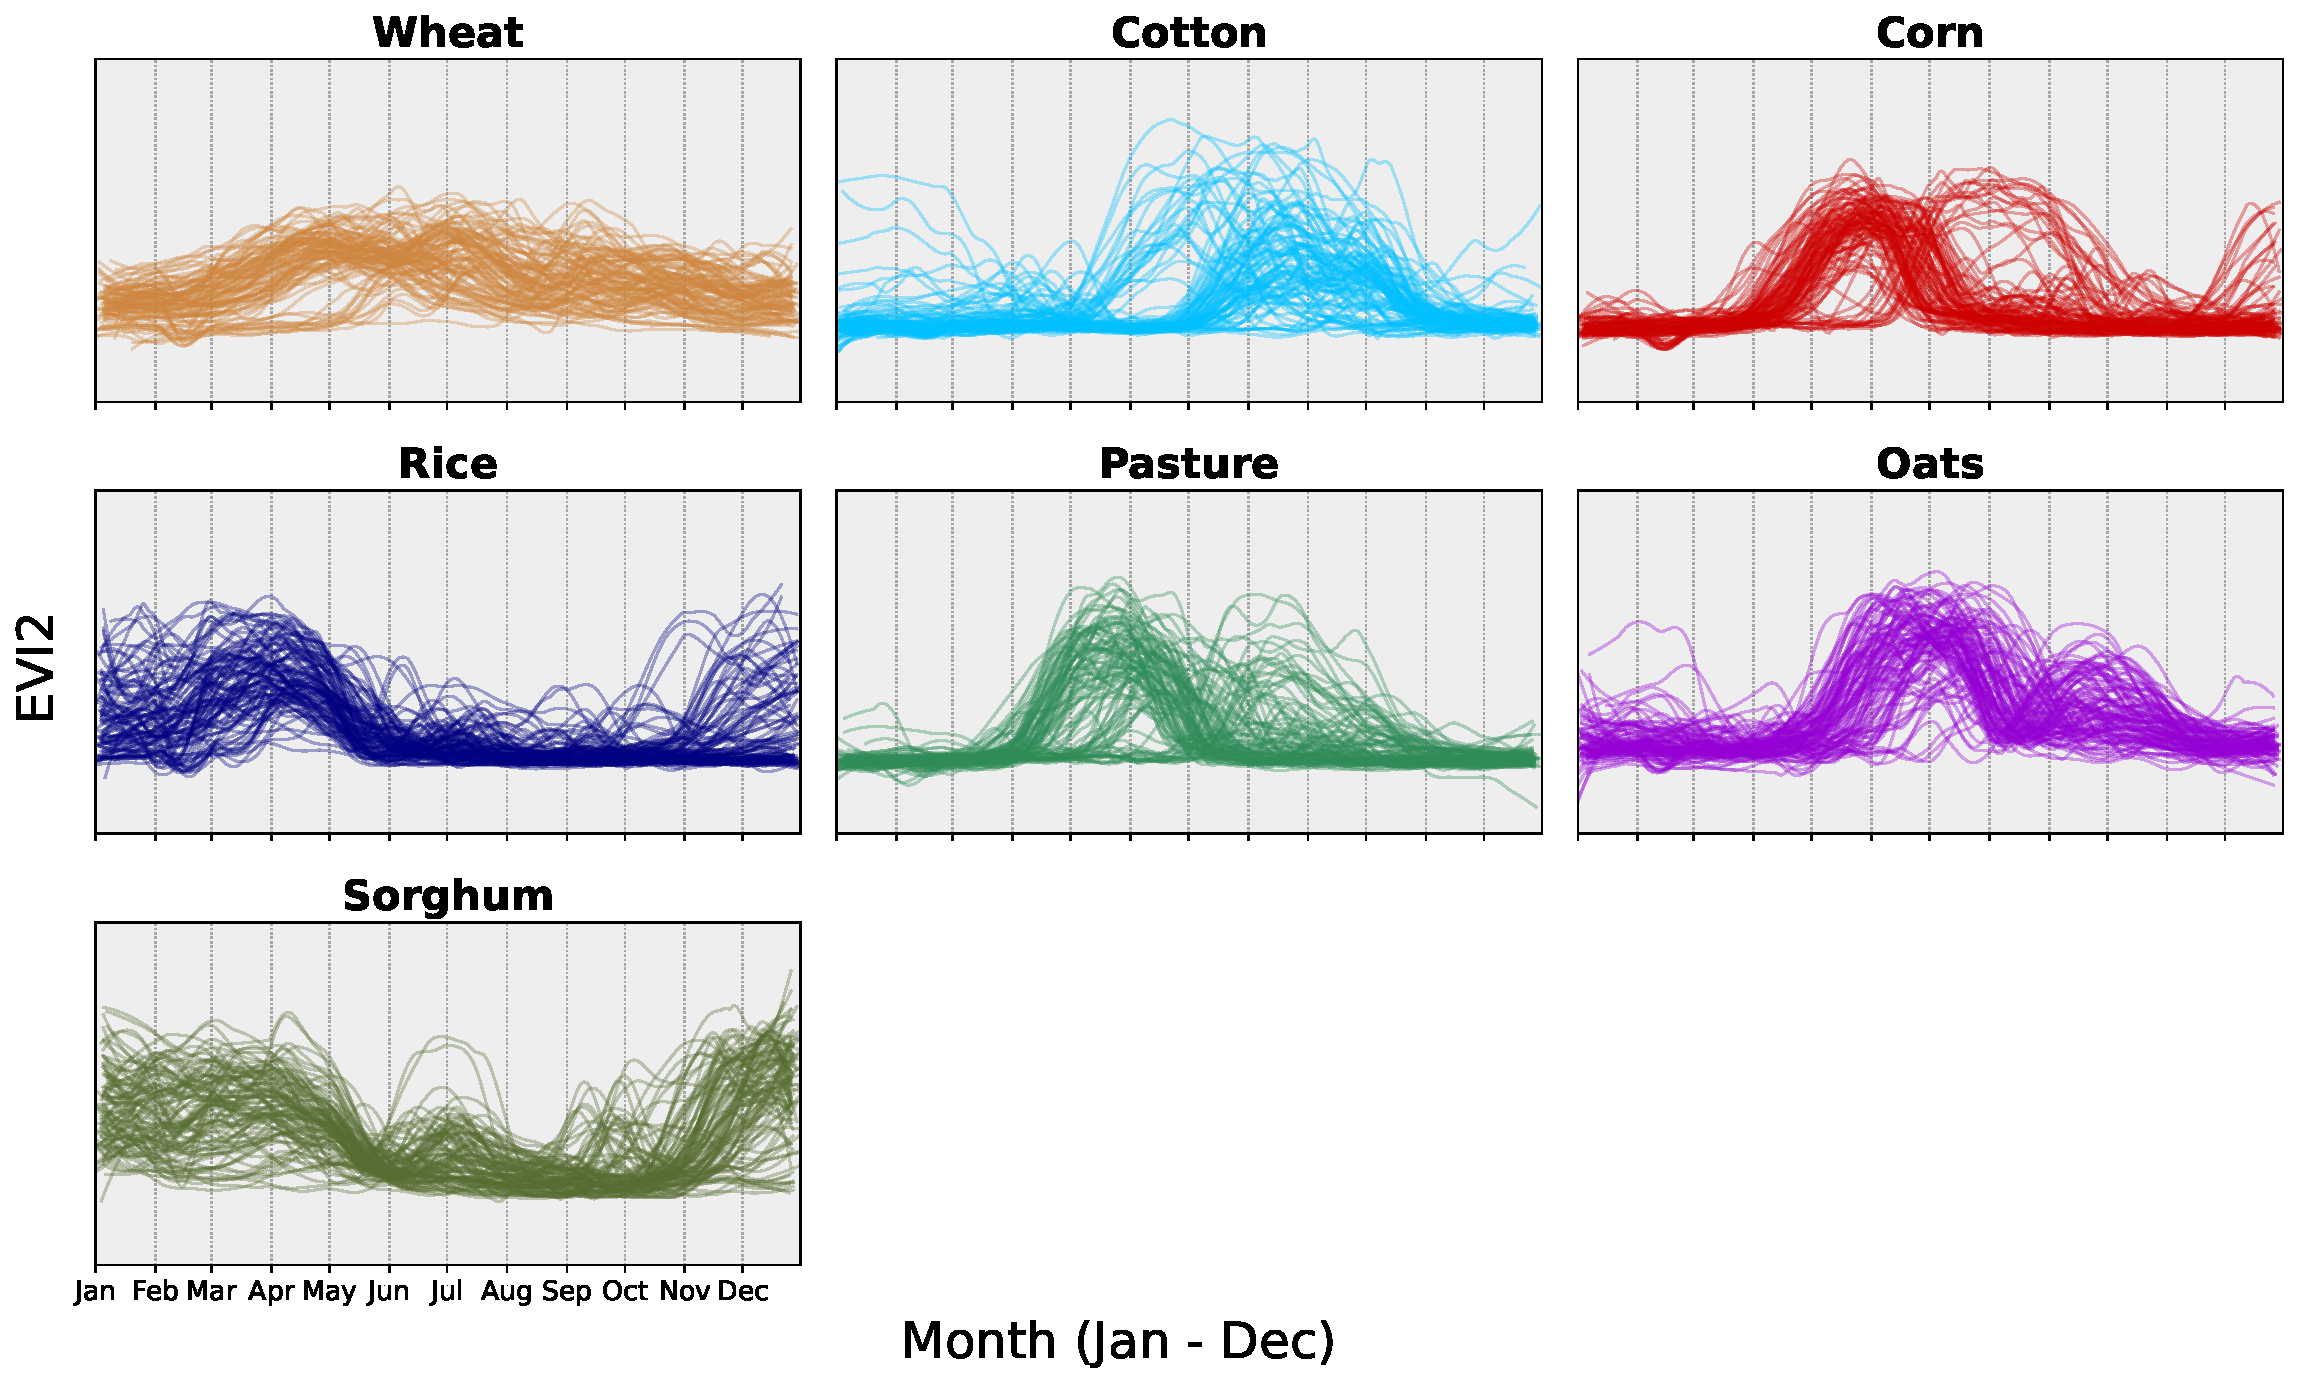
\includegraphics[height=0.4\textheight, width=\textwidth, keepaspectratio]{figures/6_methodology/datasets/texas_evi2.pdf} 
    \end{figure}
\end{frame}
\section{Methods for Learning from SITS Data}

\begin{frame}{Complete Training Pipeline Overview}
    \renewcommand{\currprop}{0.6\textheight}
    
    \begin{block}{Pretraining, Finetuning and Error Rebuttal}
        \only<1| handout:0>{During the training stage, we first retrieve the unlabeled SITS samples.}%
        \only<2| handout:0>{Samples have already been downloaded in the previous flow using our library.}%
        \only<3| handout:0>{These samples undergo data augmentation to self-supervisedly pre-train the model using SSL strategies.}%
        \only<4| handout:0>{The pre-trained backbone is then fine-tuned using a smaller, curated set of labeled samples.}%
        \only<5| handout:0>{Using these fine-tuned embeddings, we train a distinct Gaussian Mixture Model (GMM) per class for the ORDER anomaly detection framework.}%
        \only<6| handout:0>{In the inference stage, the standalone classifier makes an initial class prediction based on the time series.}%
        \only<7| handout:1>{ORDER GMM pipeline verifies the prediction, acting as a critical gatekeeper to confirm or reject the classifier's output.}%
    \end{block}
	\begin{figure}
		\centering
		\includegraphics<1| handout:0>[height=\currprop]{figures_slides/meth_graphical_abstract-6.pdf}%
		\includegraphics<2| handout:0>[height=\currprop]{figures_slides/meth_graphical_abstract-6-marked.jpg}%
		\includegraphics<3| handout:0>[height=\currprop]{figures_slides/meth_graphical_abstract-5.pdf}%
		\includegraphics<4| handout:0>[height=\currprop]{figures_slides/meth_graphical_abstract-4.pdf}%
		\includegraphics<5| handout:0>[height=\currprop]{figures_slides/meth_graphical_abstract-3.pdf}%
		\includegraphics<6| handout:0>[height=\currprop]{figures_slides/meth_graphical_abstract-2.pdf}%
        \includegraphics<7| handout:1>[height=\currprop]{figures_slides/meth_graphical_abstract-1.pdf}%
	\end{figure}
\end{frame}

% --- SHALLOW MODELS ---

\begin{frame}{Methodology: Shallow Learning Baselines}
    \begin{block}{Feature Engineering for SITS}
        Unlike deep architectures, Shallow Learning algorithms cannot natively process time series of varying lengths. To establish a baseline, we reduced the temporal dimensionality by calculating \textbf{monthly averages}, resampling the SITS to 12 fixed time steps.
    \end{block}
    
    \pause
    
    \begin{block}{Evaluated Models}
        \begin{itemize}
            \item \textbf{Random Forest (RF) \& LightGBM:} Robust ensemble methods based on decision trees.
            \item \textbf{Support Vector Machine (SVM):} Classical maximum-margin classifier.
            \item \textbf{Multi-Layer Perceptron (MLP):} A standard feed-forward neural network.
        \end{itemize}
    \end{block}
\end{frame}

\begin{frame}{Deep Learning Architectures}
    \renewcommand{\currprop}{0.6\textheight}
    
    \begin{block}{Backbone construction}
        {Let's take a closer look at the architectures of Deep Learning models.}%
    \end{block}
	\begin{figure}
		\centering
		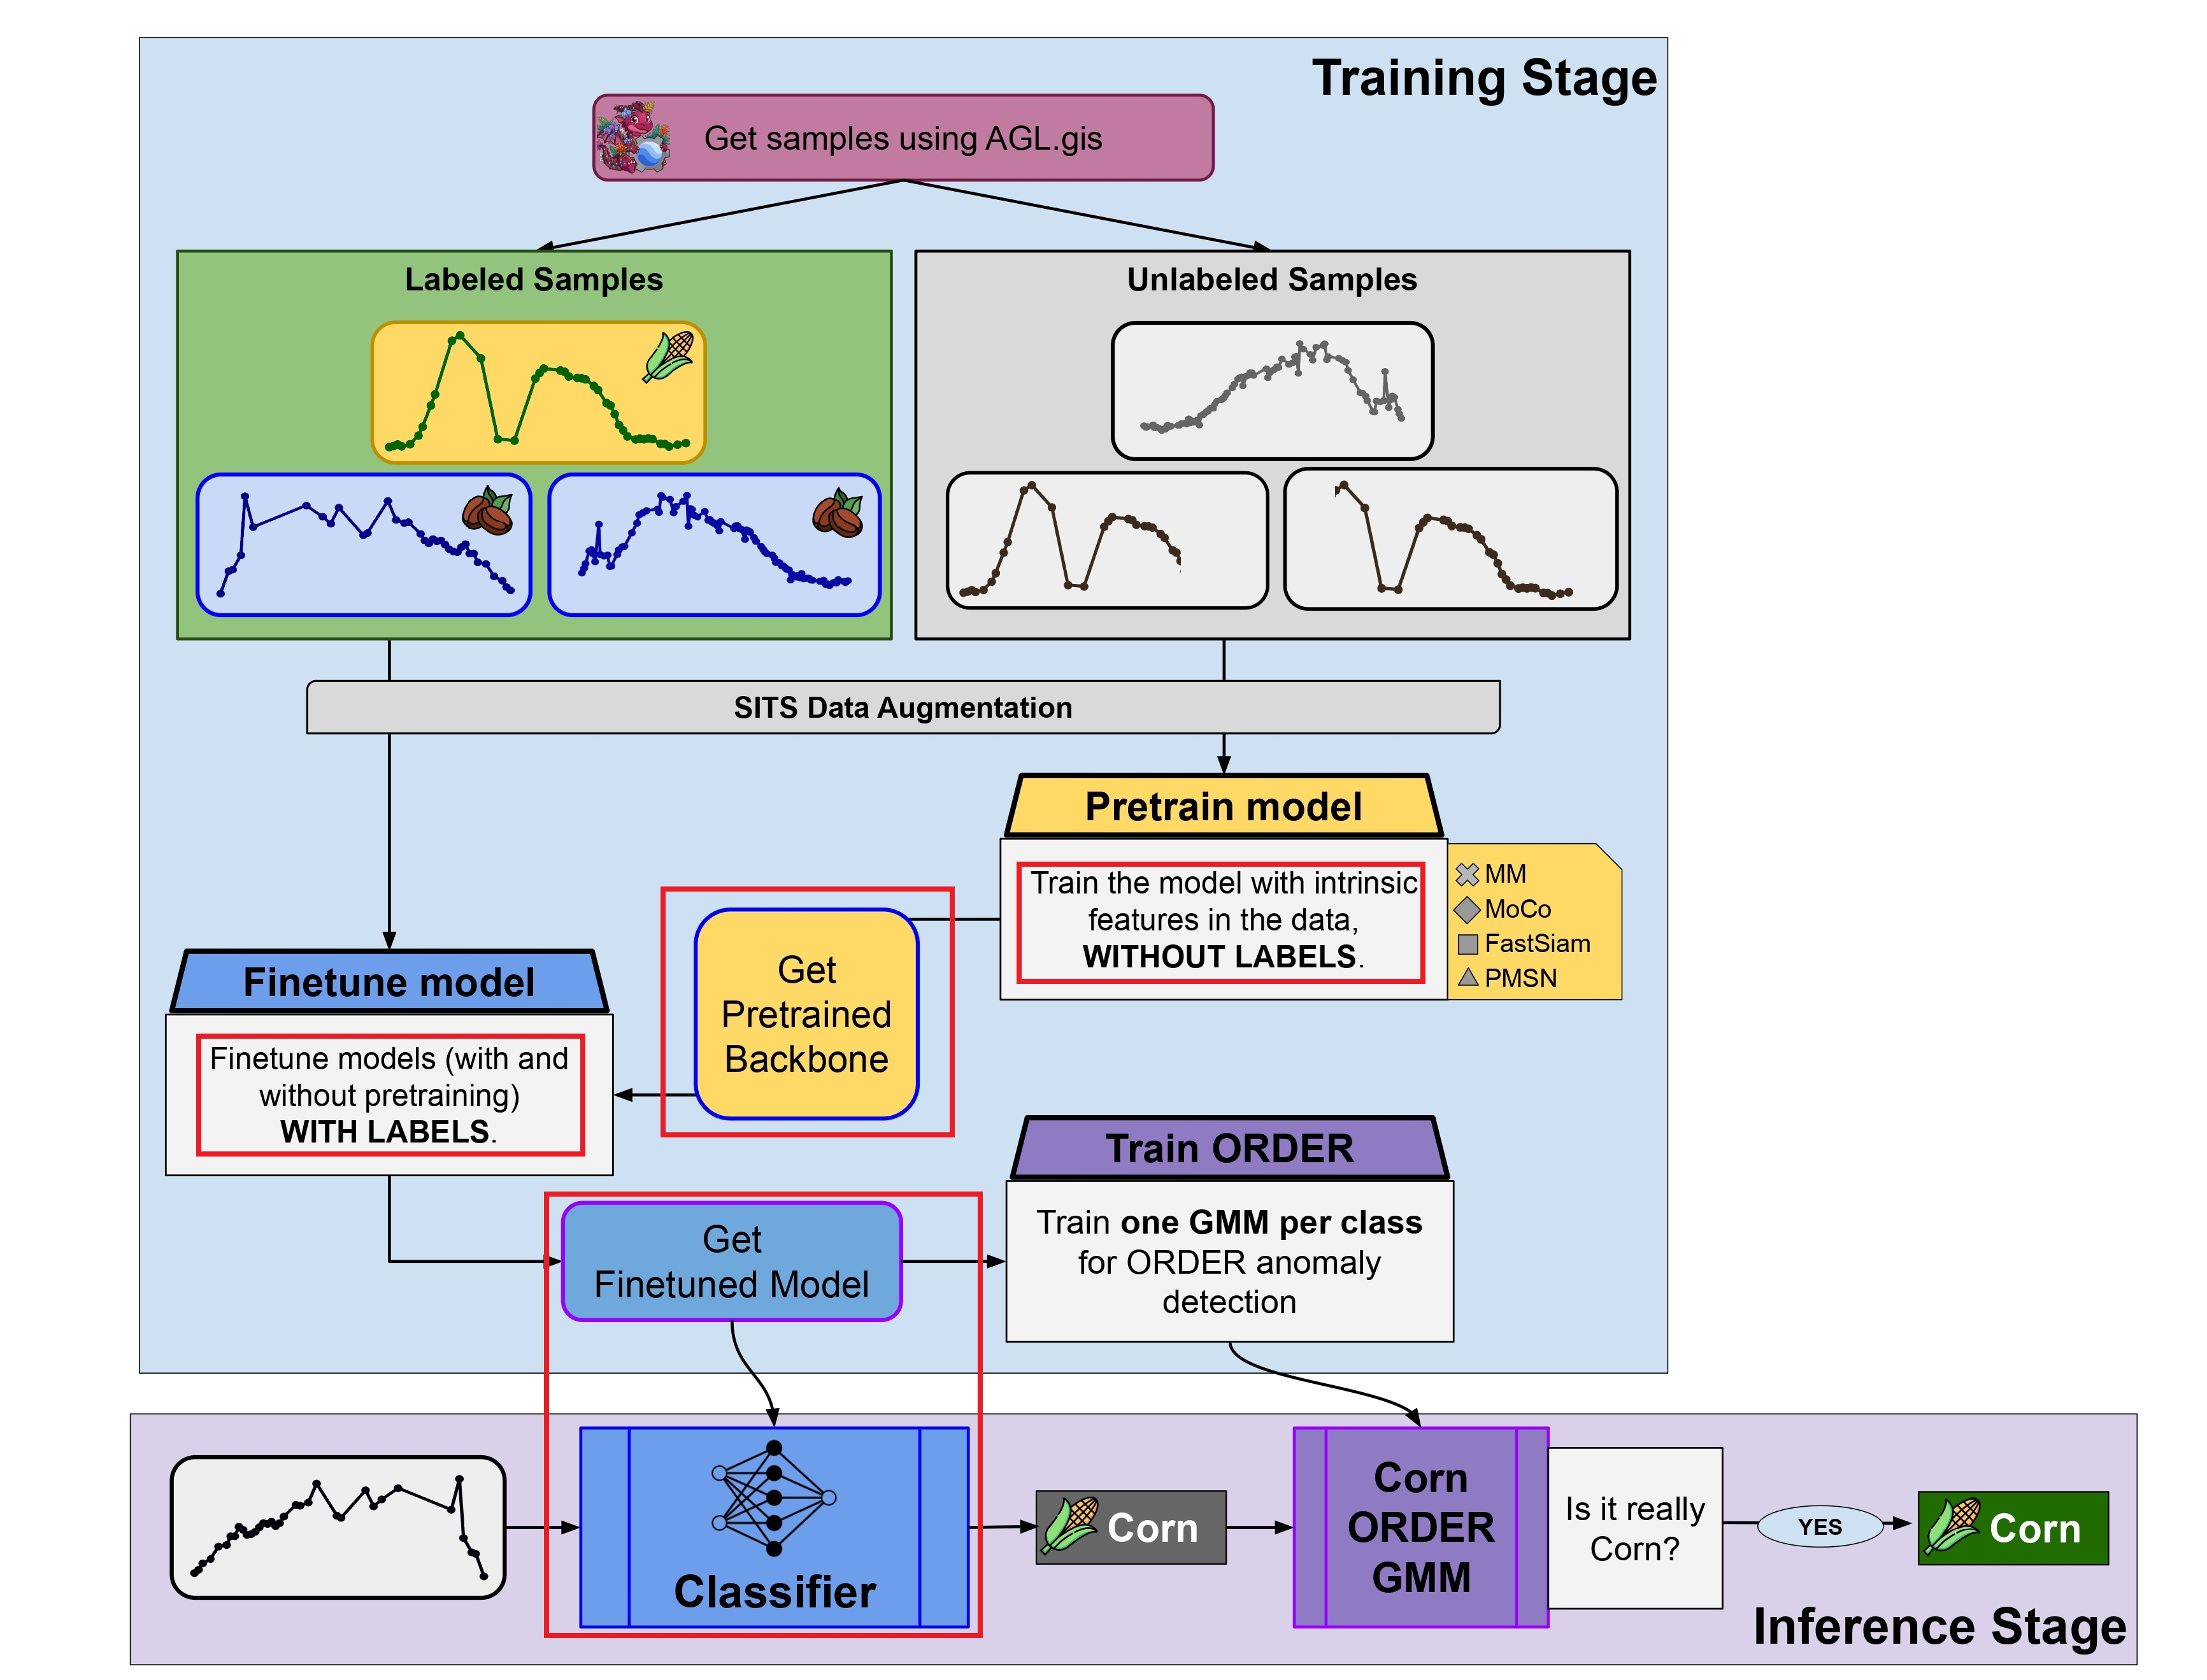
\includegraphics[height=\currprop]{figures_slides/meth_graphical_abstract_models.jpg}%
	\end{figure}
\end{frame}

\begin{frame}{Deep Learning Architectures}    
    \begin{enumerate}
        \item \textbf{SITS-CNN (ConvNeXt-based):} Adapts modern 2D vision techniques to 1D sequences, utilizing large convolutional kernels (size 7) to efficiently capture broad temporal contexts. \textbf{(Ours)}
        \item \textbf{SITS-LSTM (Recurrent):} Employs Bidirectional GRUs with early Day-of-the-Year (DoY) positional encoding, capturing forward and backward temporal dependencies for fair baseline comparisons. \textbf{(Ours)}
        \item \textbf{SITS-BERT (Transformer):} Uses standard self-attention (3 layers, 8 heads) to process the entire sequence simultaneously, fusing inputs with DoY encodings to preserve agricultural calendars. \footnote[1]{\url{https://ieeexplore.ieee.org/document/9252123}}
    \end{enumerate}
\end{frame}

\begin{frame}{Deep Learning Architectures}    
    \begin{enumerate}
        \item \textbf{SITS-BERT++ (Enhanced Transformer):} An architectural evolution of SITS-BERT featuring increased capacity (12 heads) and a dual activation strategy (Swish/GeLU) for optimized gradient flow. \footnote[1]{\url{https://ieeexplore.ieee.org/document/10899708}}
        \item \textbf{SITS-Mamba (State Space Model):} A lightweight, post-Transformer approach using Selective State Spaces (S6) to filter irrelevant data, offering high-level reasoning with linear $\mathcal{O}(L)$ efficiency. \textbf{(Ours)}
    \end{enumerate}
\end{frame}

\begin{frame}{SSL Pretrain}
    \renewcommand{\currprop}{0.6\textheight}
    
    \begin{block}{Better than random weights}
        {Let's take a closer look how SSL pretraining works in the pipeline.}%
    \end{block}
	\begin{figure}
		\centering
		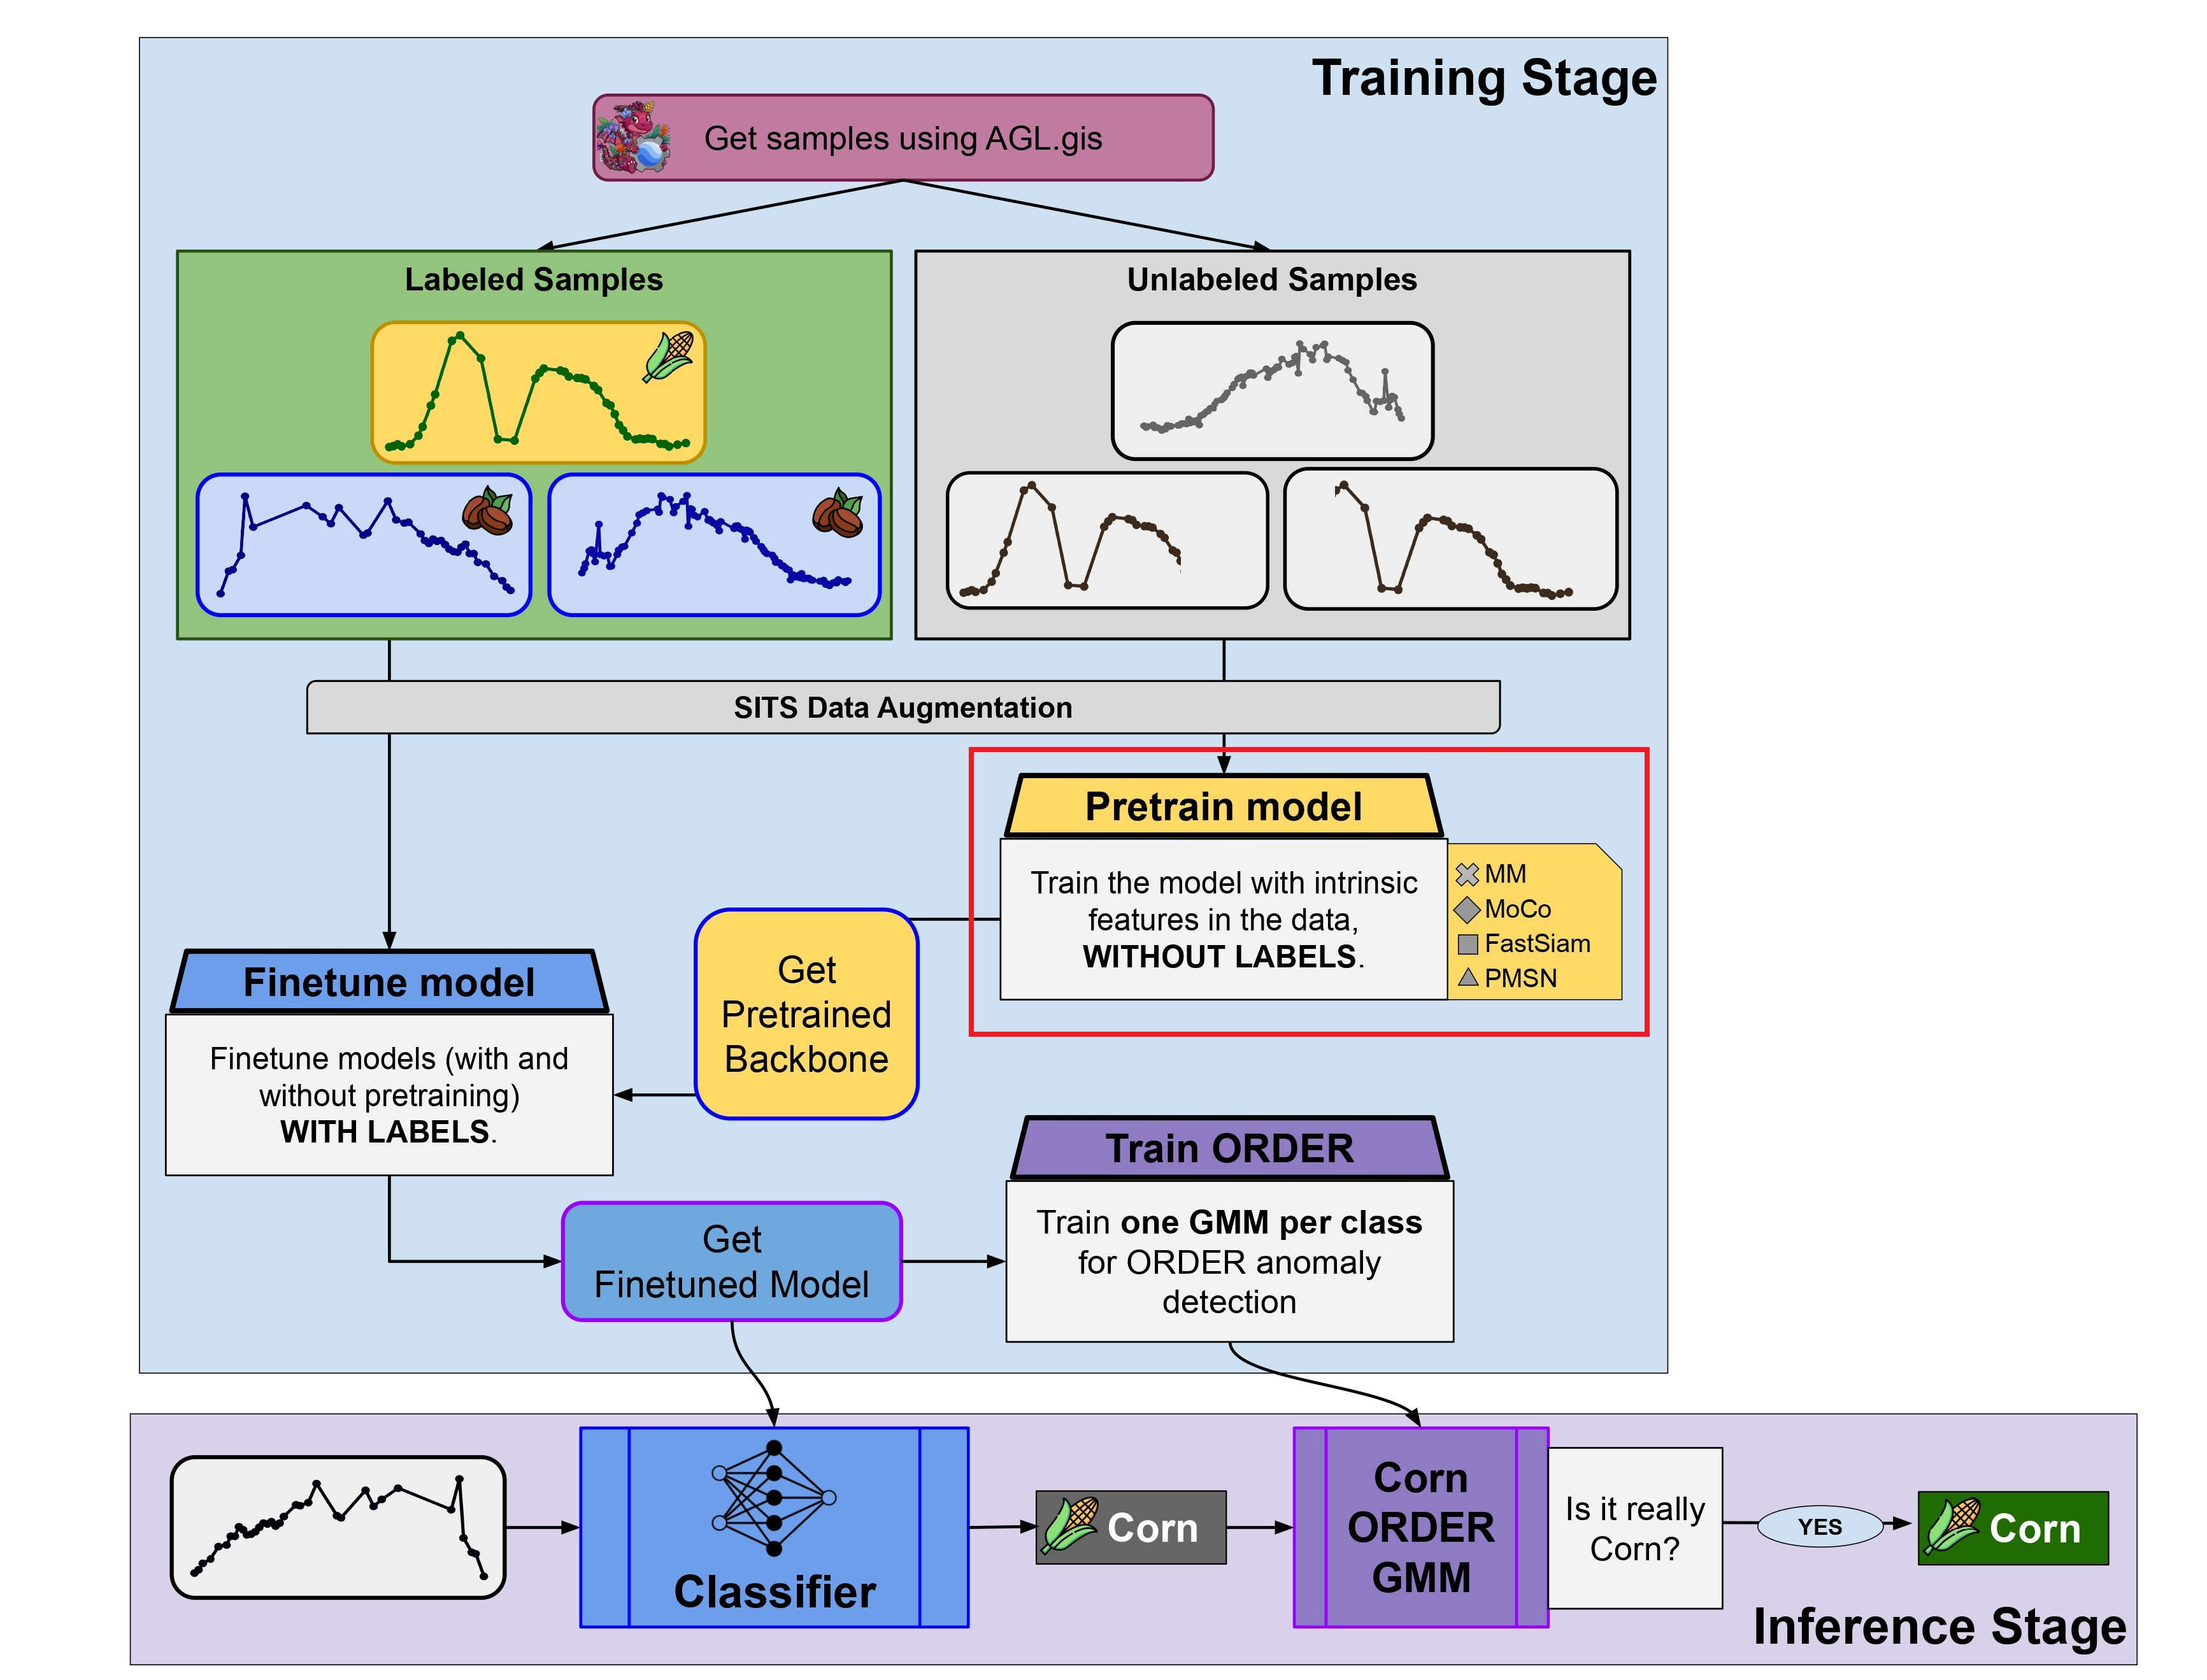
\includegraphics[height=\currprop]{figures_slides/meth_graphical_abstract_ssl.jpg}%
	\end{figure}
\end{frame}

\begin{frame}{SSL Pretrain}
    \renewcommand{\currprop}{0.5\textheight}
    
    \begin{block}{Deep Feature Extraction from Pretrained Networks}
        \only<1| handout:0>{The self-supervised learning process begins with an original, unlabeled SITS sample.}%
        \only<2| handout:0>{Data augmentation techniques generate distinct altered views of this same original sequence.}%
        \only<3| handout:0>{Driven by the FastSiam architecture, the model forces these augmented views closer together in the pre-training embedding space.}%
        \only<4| handout:0>{Simultaneously, a database of negative samples provides distinct, unrelated time series for contrastive learning.}%
        \only<5| handout:0>{Applying the MoCo paradigm, the model actively pushes these negative embeddings far away from the positive anchor.}%
        \only<6| handout:0>{A Masked Modeling (MM) approach further challenges the network by dropping random temporal segments from the signal.}%
        \only<7| handout:0>{The network learns intrinsic structural patterns by attempting to accurately reconstruct these masked segments.}%
        \only<8| handout:1>{Ultimately, the PMSN strategy unifies these tasks—pulling similar views, pushing negative samples, and reconstructing masks—into a single, pre-training mechanism.}%
    \end{block}
	\begin{figure}
		\centering
		\includegraphics<1| handout:0>[height=\currprop]{figures_slides/meth_ssl-7.pdf}%
		\includegraphics<2| handout:0>[height=\currprop]{figures_slides/meth_ssl-6.pdf}%
        \includegraphics<3| handout:0>[height=\currprop]{figures_slides/meth_ssl-5.pdf}%
        \includegraphics<4| handout:0>[height=\currprop]{figures_slides/meth_ssl-4.pdf}%
        \includegraphics<5| handout:0>[height=\currprop]{figures_slides/meth_ssl-3.pdf}%
        \includegraphics<6| handout:0>[height=\currprop]{figures_slides/meth_ssl-2.pdf}%
        \includegraphics<7| handout:0>[height=\currprop]{figures_slides/meth_ssl-1.pdf}%
        \includegraphics<8| handout:1>[height=\currprop]{figures_slides/meth_ssl.pdf}%
	\end{figure}
\end{frame}

\begin{frame}{ORDER - In details}
    \renewcommand{\currprop}{0.6\textheight}
    
    \begin{block}{The Last Step}
        {Let's take a closer look how ORDER anomaly detection works in the pipeline.}%
    \end{block}
	\begin{figure}
		\centering
		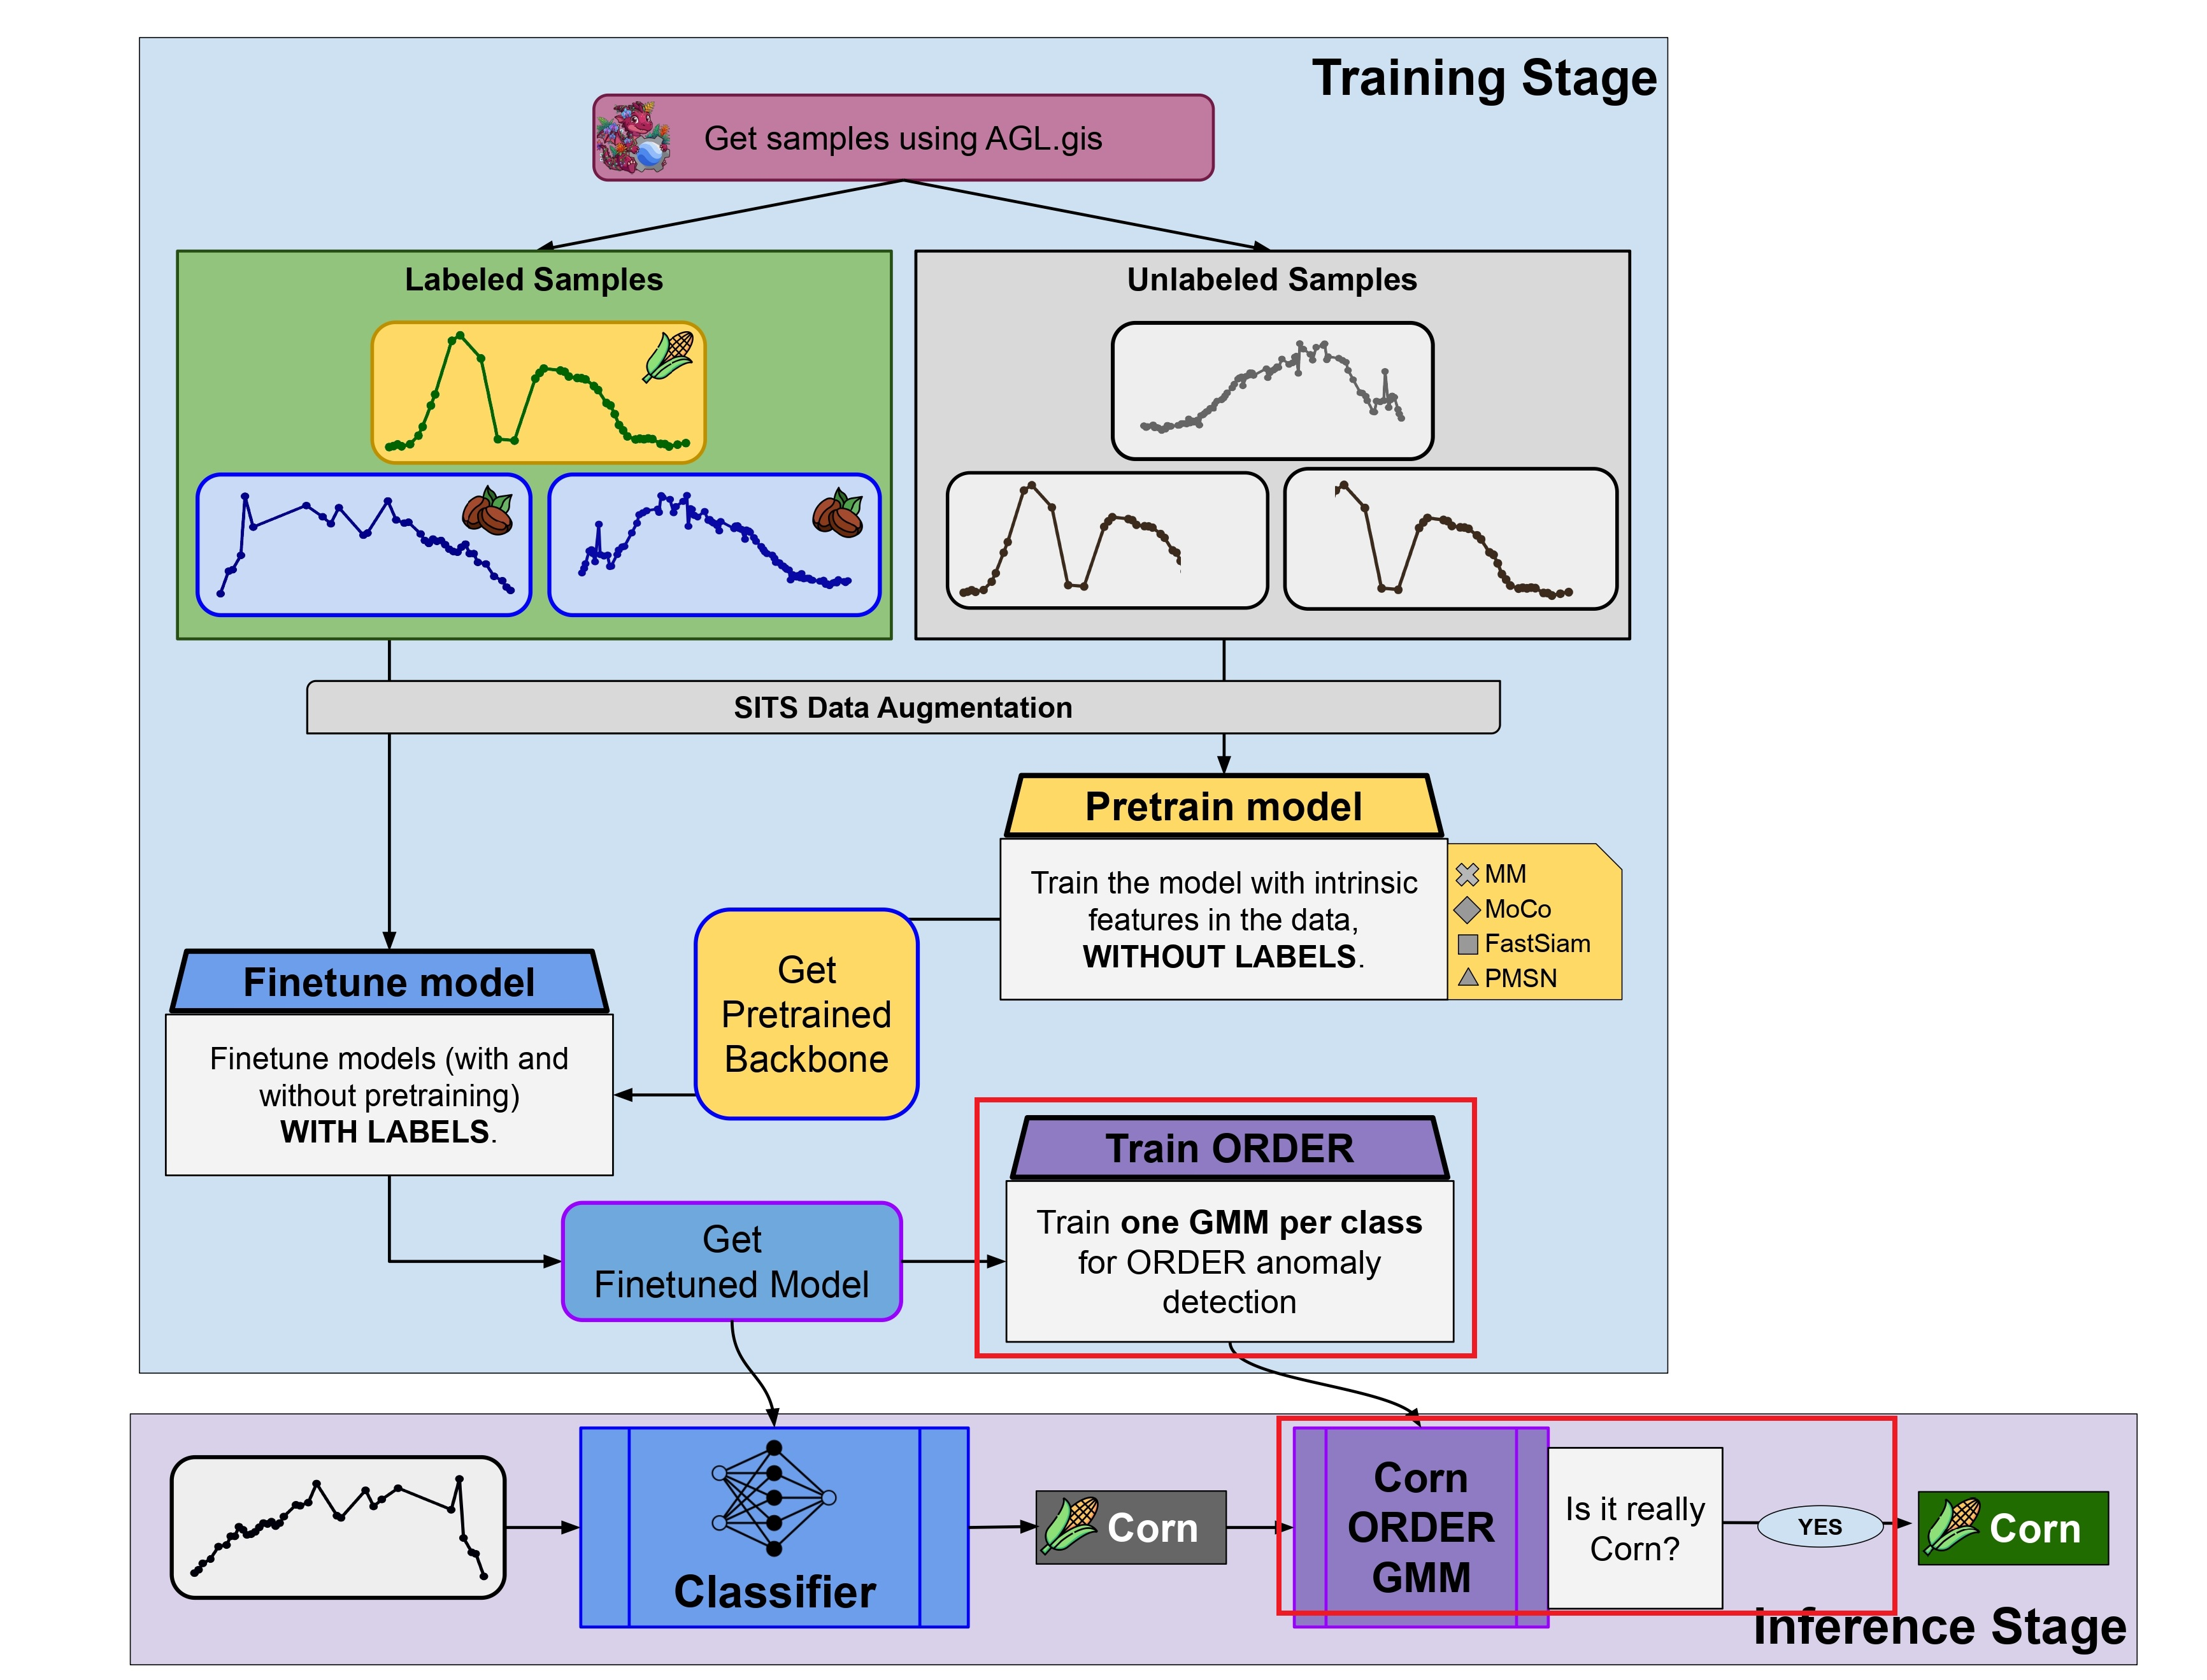
\includegraphics[height=\currprop]{figures_slides/meth_graphical_abstract_order.jpg}%
	\end{figure}
\end{frame}

\begin{frame}{ORDER - In details}
    \renewcommand{\currprop}{0.5\textheight}
    
    \begin{block}{Open-set Recognition for Discriminative Error Rebutta}
        \only<1| handout:0>{The system utilizes the trainig and validation dataset to pass representations through the fine-tuned model backbone.}%
        \only<2| handout:0>{Within the embedding space, the training samples initialize one distinct GMM for each crop class.}%
        \only<3| handout:0>{Both positive and negative validation samples are subsequently mapped to evaluate these class boundaries.}%
        \only<4| handout:0>{The hyperparameter optimization loop begins by scoring all validation sets against the fitted GMMs.}%
        \only<5| handout:0>{This process actively maximizes the spatial separation between clean predictions and hard, out-of-distribution samples.}%
        \only<6| handout:0>{A dynamic confidence threshold is statistically determined for each class by maximizing the F1-score.}%
        \only<7| handout:0>{To ensure ultimate reliability, a conservative fallback mechanism (GEMOS) is integrated for cases with very few correct or incorrect validation samples.}%
        \only<8| handout:0>{During class fixation, the system evaluates: 'Is the GMM score greater than the dynamic threshold?'}%
        \only<9| handout:0>{At inference time, unseen time-series samples are projected into the classifier embedding space, as usual.}%
        \only<10| handout:0>{The fine-tuned classification head assigns a preliminary label to the new inference sample.}%
        \only<11| handout:1>{If the score exceeds the threshold, the prediction is trusted; otherwise, the sample is safely flagged as Unknown.}%
    \end{block}
	\begin{figure}
		\centering
		\includegraphics<1| handout:0>[height=\currprop]{figures_slides/meth_models-10.pdf}%
		\includegraphics<2| handout:0>[height=\currprop]{figures_slides/meth_models-9.pdf}%
		\includegraphics<3| handout:0>[height=\currprop]{figures_slides/meth_models-8.pdf}%
		\includegraphics<4| handout:0>[height=\currprop]{figures_slides/meth_models-7.pdf}%
		\includegraphics<5| handout:0>[height=\currprop]{figures_slides/meth_models-6.pdf}%
        \includegraphics<6| handout:0>[height=\currprop]{figures_slides/meth_models-5.pdf}%
        \includegraphics<7| handout:0>[height=\currprop]{figures_slides/meth_models-4.pdf}%
        \includegraphics<8| handout:0>[height=\currprop]{figures_slides/meth_models-3.pdf}%
        \includegraphics<9| handout:0>[height=\currprop]{figures_slides/meth_models-2.pdf}%
        \includegraphics<10| handout:0>[height=\currprop]{figures_slides/meth_models-1.pdf}%
        \includegraphics<11| handout:1>[height=\currprop]{figures_slides/meth_models.pdf}%
	\end{figure}
\end{frame}
\section{Experimental Setup}
\label{sec:06:setup}

\begin{frame}{Experimental Setup: Evaluation Scenarios \& Models}
    \begin{block}{Data Scarcity Regimes}
        To evaluate model robustness and the impact of Self-Supervised Learning, we simulated different label availability scenarios: \textbf{70\%} (traditional regime), \textbf{10\%}, \textbf{1\%}, and \textbf{0.1\%} (\textit{few-shot} regimes) of the training data \textbf{(RQ2)}.
    \end{block}

    \vspace{0.2cm}

    \begin{block}{Training Details}
        DL models were optimized using \textbf{AdamW}\footnote[1]{\url{https://arxiv.org/abs/1711.05101}} with a cosine annealing learning rate scheduler and Early Stopping. Conversely, SL models underwent Tree-structured Parzen Estimator\footnote[2]{\url{https://arxiv.org/abs/2304.11127}} hyperparameter search.
    \end{block}
\end{frame}

\begin{frame}{Experimental Setup: Anomaly Detection (ORDER)}
    \begin{block}{Confidence Estimation Baselines}
        To evaluate the proposed \textbf{ORDER} \textbf{(RQ5)} method in detecting classification failures, we established two main baselines:
        \begin{itemize}
            \item \textbf{MCP (Maximum Class Probability):} The standard Softmax confidence.
            \item \textbf{ConfidNet:} An auxiliary neural network specifically trained to predict the True Class Probability (TCP) of the main classifier.
        \end{itemize}
    \end{block}

\end{frame}

\section{Results}

% --- SLIDE 1: SUPERVISED BASELINES (TABELAS 6, 7, 8) ---

\subsection{Traditional Regime}

\begin{frame}{Traditional Regime}
    DL models (Transformers and Mamba) consistently outperform SL models with 70\% of labels without pretraining.

    \vspace{0.2cm}

    \begin{table}[h]
        \centering
        \resizebox{0.9\textwidth}{!}{%
        \begin{tabular}{c|l|ccc}
        \hline
        \textbf{Type} & \textbf{Model} & \textbf{Brazil (F1)} & \textbf{Texas (F1)} & \textbf{California (F1)} \\ \hline
        \multirow{3}{*}{Shallow} & SVM & 77.7\% & 98.8\% & 97.2\% \\
         & Random Forest & 75.0\% & 97.9\% & 95.3\% \\
         & MLP & 79.2\% & 99.1\% & 97.0\% \\ \hline
        \multirow{4}{*}{Deep} & SITS-CNN & 83.8\% & 99.5\% & \textbf{98.2\%} \\
         & SITS-LSTM & 84.6\% & \textbf{99.6\%} & 97.4\% \\
         & SITS-BERT++ & \textbf{85.6\%} & 99.5\% & 97.7\% \\
         & SITS-Mamba & 85.0\% & \textbf{99.6\%} & 97.9\% \\ \hline
        \end{tabular}%
        }
    \end{table}
\end{frame}

% --- SLIDE 3: FEW SHOT REGIMES (FIGURAS 54, 55, 56) ---

\subsection{Few Shot Regime}

\begin{frame}{Few Shot Regime}
    \begin{block}{The Impact of SSL in Data Scarcity}
        MoCo pre-training boosts F1-Scores by up to 40\% compared to random initialization.
    \end{block}

    \vspace{0.2cm}

    \begin{figure}
        \centering
        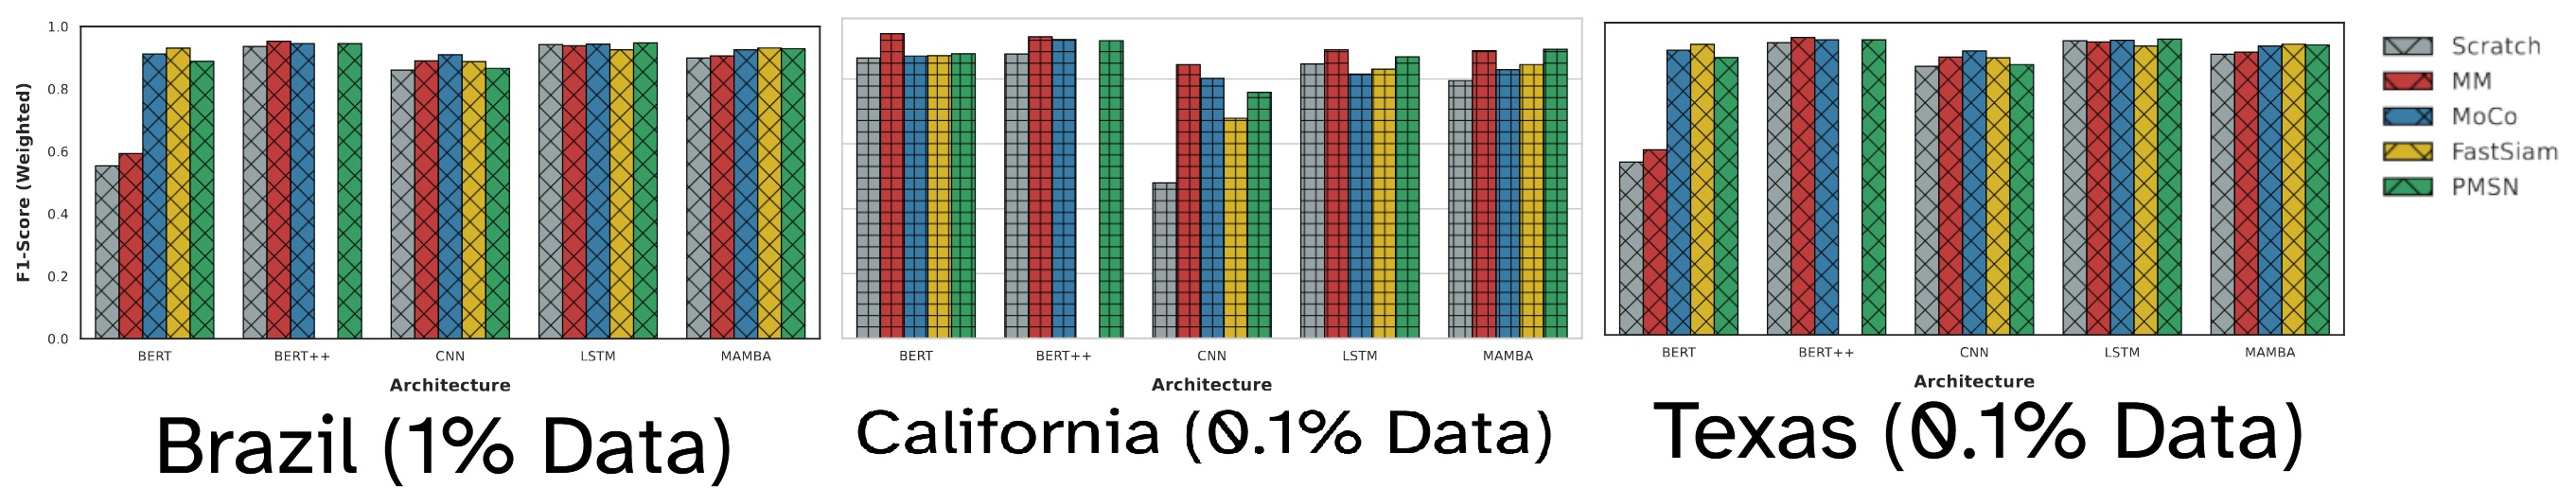
\includegraphics[width=\textwidth, keepaspectratio]{figures_slides/slide_few_shot.jpg}
    \end{figure}
    
\end{frame}

% --- SLIDE 4: DATA SCALING (FIGURAS 57, 58, 59) ---

\begin{frame}{Scaling the Training Data (1\% $\rightarrow$ 10\% $\rightarrow$ 70\%)}
    \begin{block}{Convergence Phenomenon}
        As the availability of labeled data scales to 70\%, the strong supervised signal overrides the SSL initialization, making pre-training less critical. % Architectures like SITS-BERT heavily rely on SSL to avoid poor fitting in few-shot scenarios.
    \end{block}
    
    \vspace{0.2cm}

    \begin{figure}[ht]
        \centering
        % Primeira "coluna" para a Imagem
        \begin{minipage}{0.75\textwidth}
            \centering
            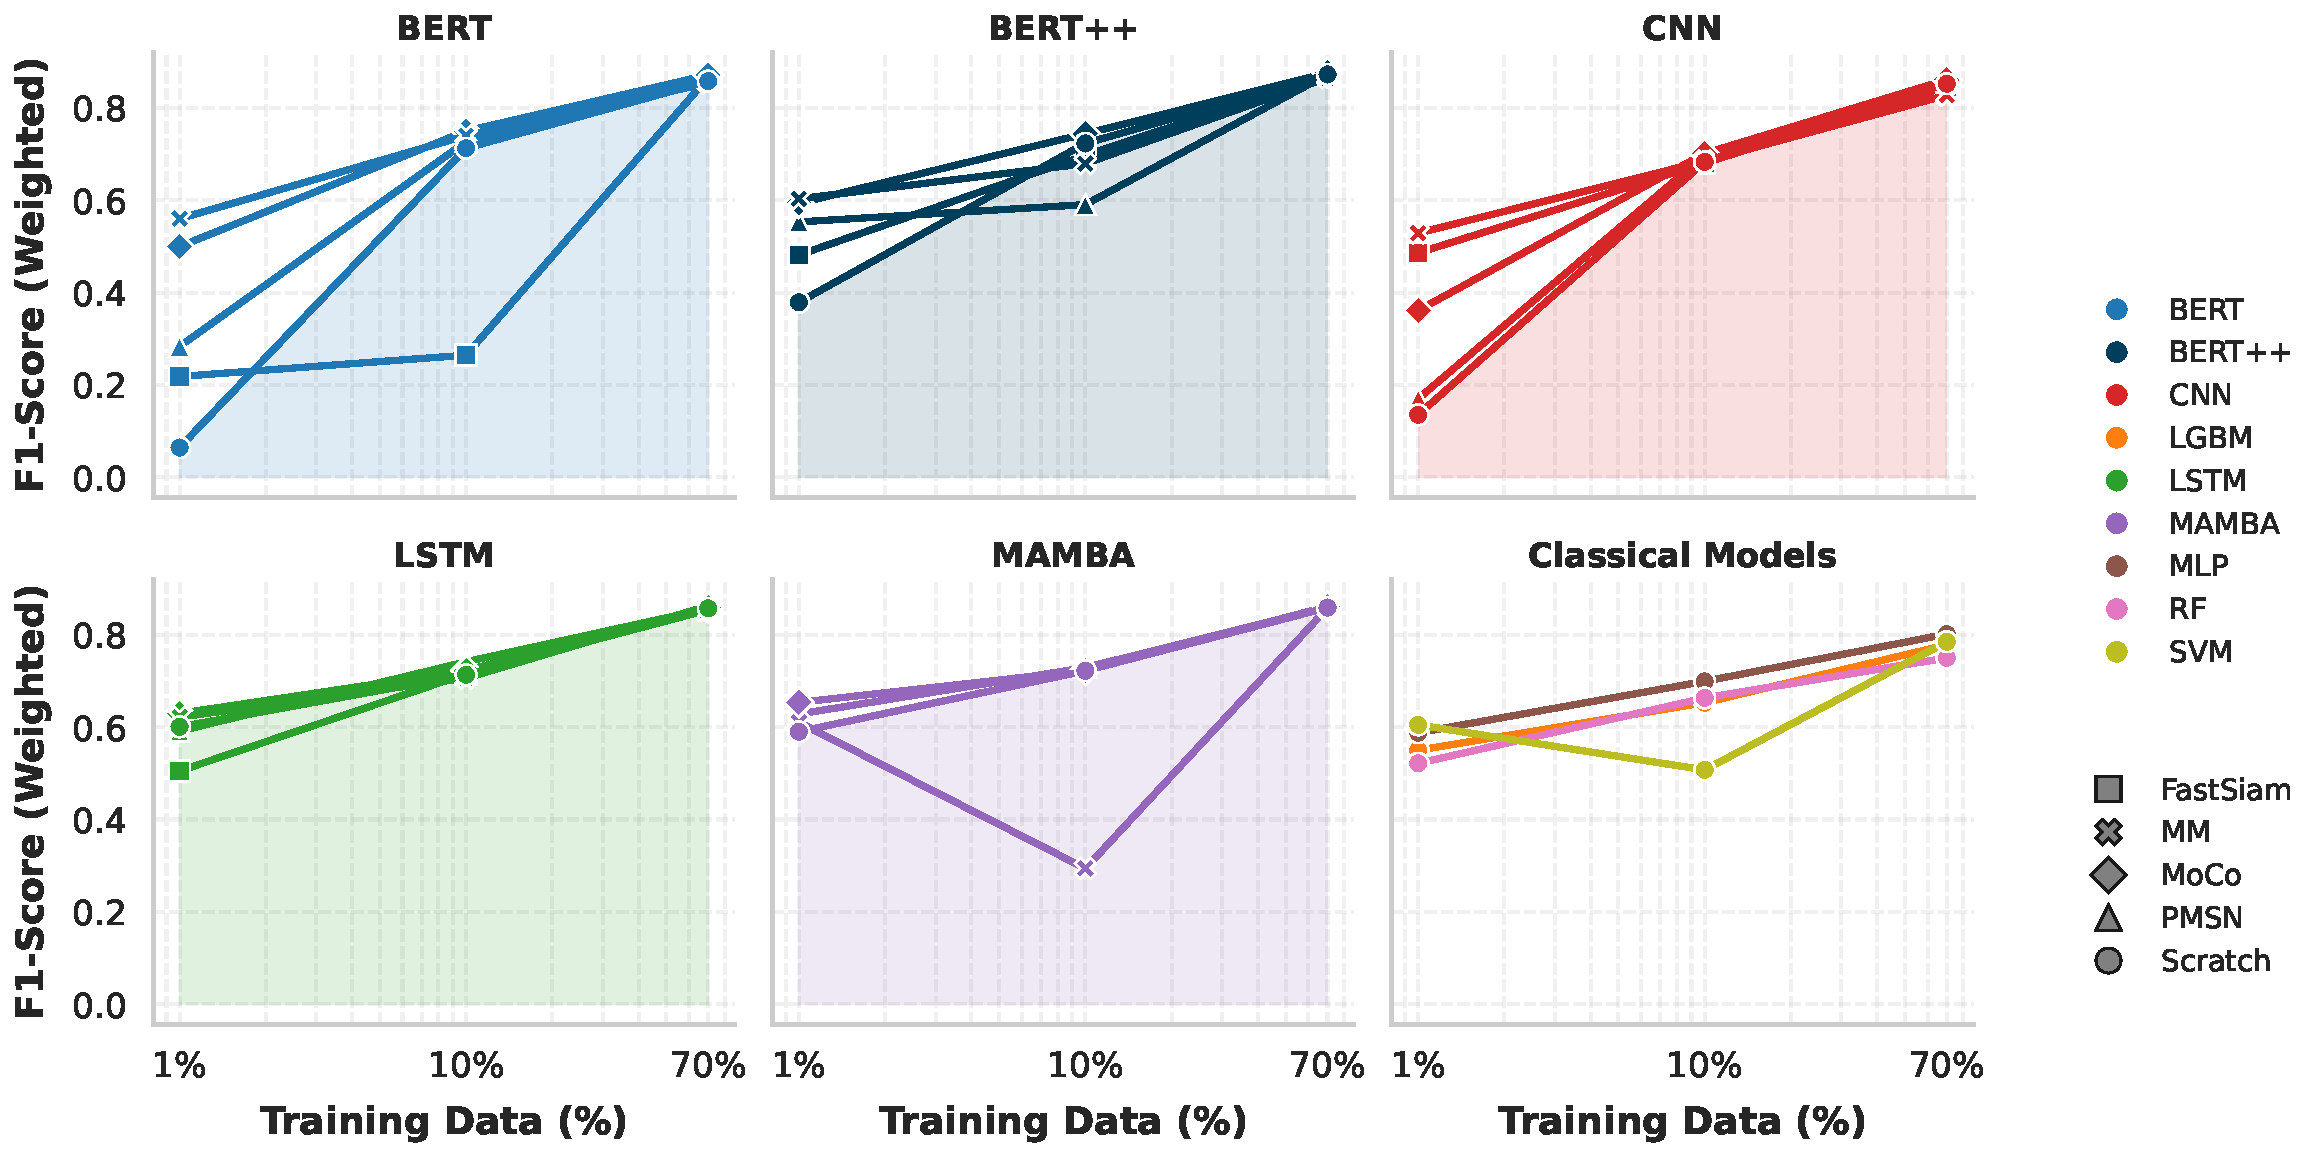
\includegraphics[width=\textwidth, keepaspectratio]{figures/8_results/brazil-finetuning/line_training.pdf}
        \end{minipage}
        \hfill
        \begin{minipage}{0.20\textwidth}
            \caption*{Brazil}
        \end{minipage}
    \end{figure}

\end{frame}

\begin{frame}{Scaling the Training Data (1\% $\rightarrow$ 10\% $\rightarrow$ 70\%)}
    \begin{block}{Convergence Phenomenon}
        The same occurs in the US datasets, although the gain is more marginal.
    \end{block}
    
    \vspace{0.2cm}

    \begin{figure}[ht]
        \centering
        % Primeira "coluna" para a Imagem
        \begin{minipage}{0.75\textwidth}
            \centering
            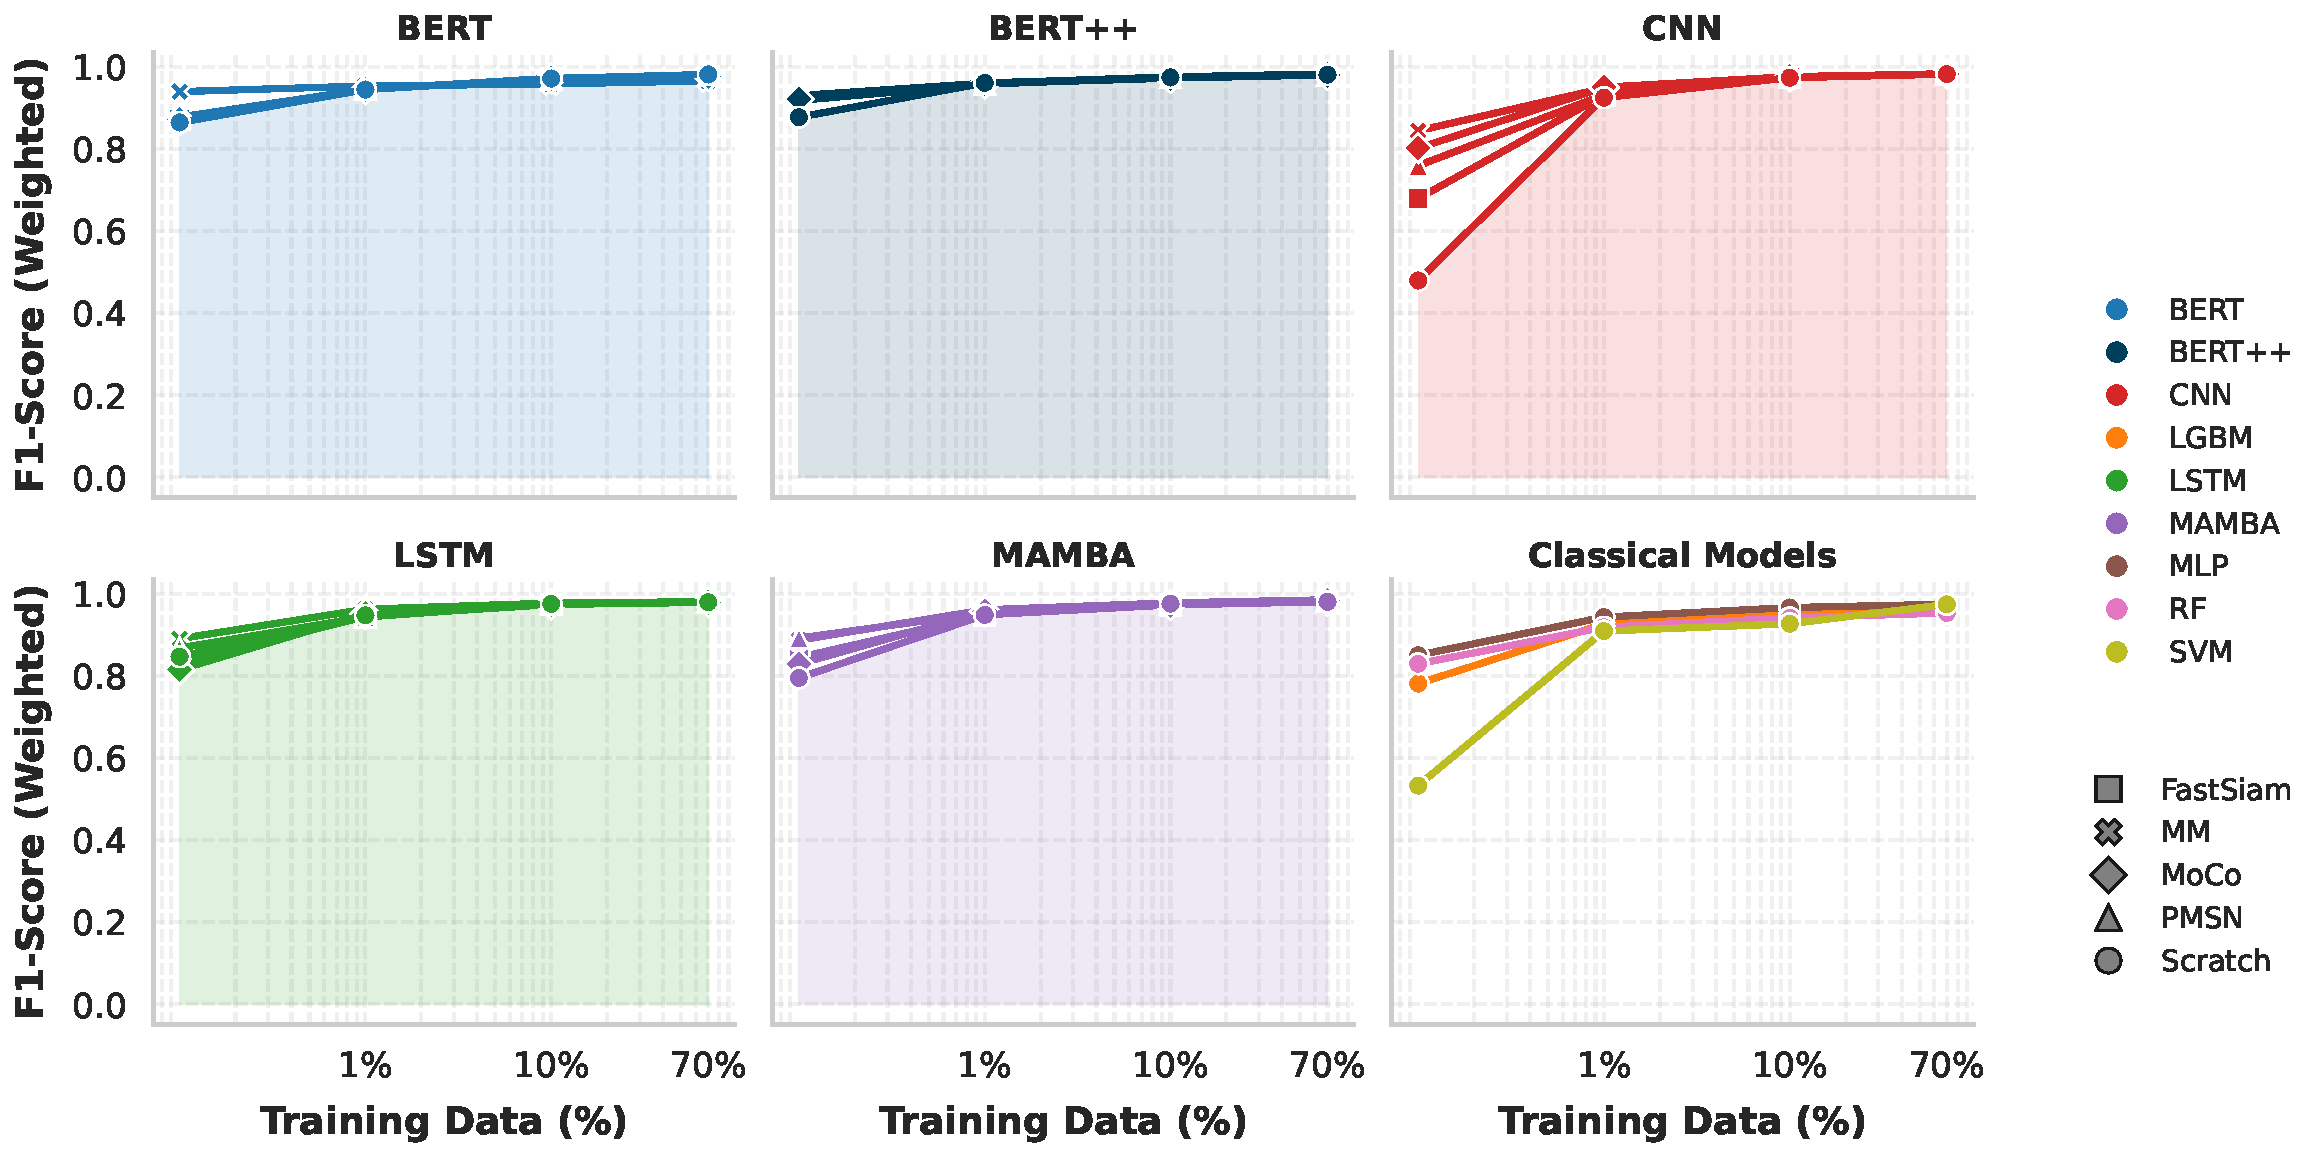
\includegraphics[width=\textwidth, keepaspectratio]{figures/8_results/california-finetuning/line_training.pdf}
        \end{minipage}
        \hfill
        \begin{minipage}{0.20\textwidth}
            \caption*{California}
        \end{minipage}
    \end{figure}

\end{frame}

% --- SLIDE 5: ORDER OVERVIEW (FIGURAS 60, 61, 62) ---

\begin{frame}{Anomaly Detection: The ORDER Method Overview}
    \begin{block}{Rebutting Classification Errors}
        Removing 5\% to 8\% of anomalies in Brazil raised the F1-Score from $\sim84\%$ to $\sim88\%$. In high-accuracy US regimes, ORDER acts remove far fewer samples. %safely and conservatively, targeting genuine label noise without degrading the boundaries.
    \end{block}
    
    \vspace{0.2cm}
    
    \begin{figure}
        \centering
        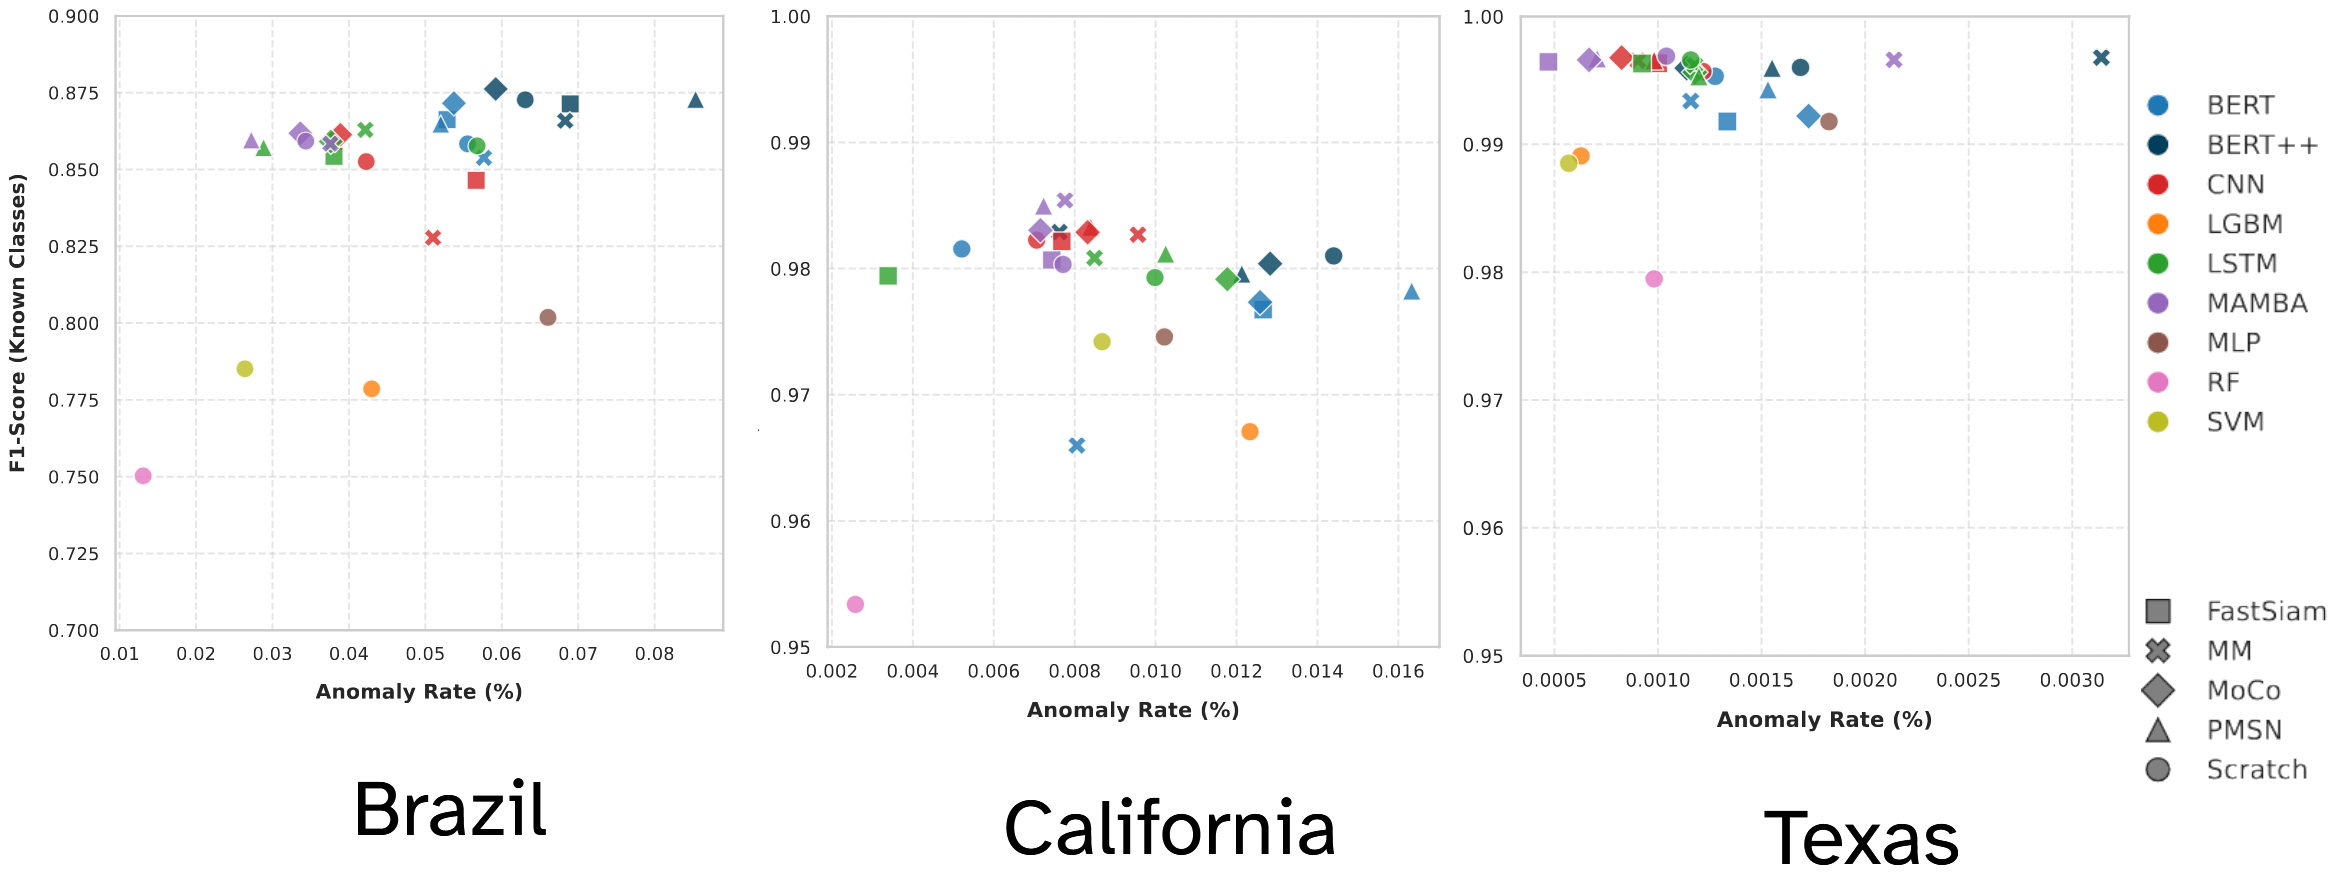
\includegraphics[width=\textwidth, keepaspectratio]{figures_slides/order_slides.jpg}
    \end{figure}

\end{frame}

\subsection{Linear Probing}

\begin{frame}{Self-Supervised Pre-training: Embeddings Quality}
    \begin{block}{Linear Evaluation (KNN F1-Score on Validation Data)}
        Evaluating the latent space via KNN reveals that \textbf{MoCo} generates consistently robust representations across all regions. %\textbf{Masked Modeling (MM)} excels in California, while \textbf{FastSiam} faces collapse issues.% in Transformers/Mamba but performs well with LSTMs.
    \end{block}
    
    \vspace{0.2cm}
    
    \begin{table}[]
        \centering
        \resizebox{0.95\textwidth}{!}{%
        \begin{tabular}{l|ccc}
        \hline
        \textbf{Best Pre-training setups} & \textbf{Brazil (1\%)} & \textbf{Texas (0.1\%)} & \textbf{California (0.1\%)} \\ \hline
        \textbf{MoCo} (Contrastive) & \textbf{63.80\%} (BERT) & \textbf{88.38\%} (Mamba) & 82.98\% (Mamba) \\
        \textbf{MM} (Reconstruction) & 62.18\% (BERT) & 85.25\% (BERT) & \textbf{85.77\%} (LSTM) \\
        \textbf{FastSiam} (Non-Contrastive) & 58.36\% (Mamba) & 87.84\% (LSTM) & 82.38\% (Mamba) \\
        \textbf{PMSN} (Hybrid) & 61.23\% (LSTM) & 88.54\% (BERT++) & 81.45\% (Mamba) \\ \hline
        \end{tabular}%
        }
    \end{table}
\end{frame}

% --- SLIDE 6: BEST RESULT BRAZIL (FIGURAS 63, 64) ---

\subsection{Best Results per Dataset}

\begin{frame}{Best Setup: Brazil Dataset}
    \begin{block}{SITS-BERT++ (MoCo Pre-training)}
        Aside the agricultural complexity of the Brazil dataset, our pipeline achieve far results.% the SITS-BERT++ model with MoCo pre-training establishes a robust baseline despite inherent confusion in challenging classes like Pasture and Temporary Crops..
    \end{block}
    
    \vspace{0.2cm}
    
    \begin{columns}[T]
        \begin{column}{0.48\textwidth}
            \begin{figure}
                \centering
                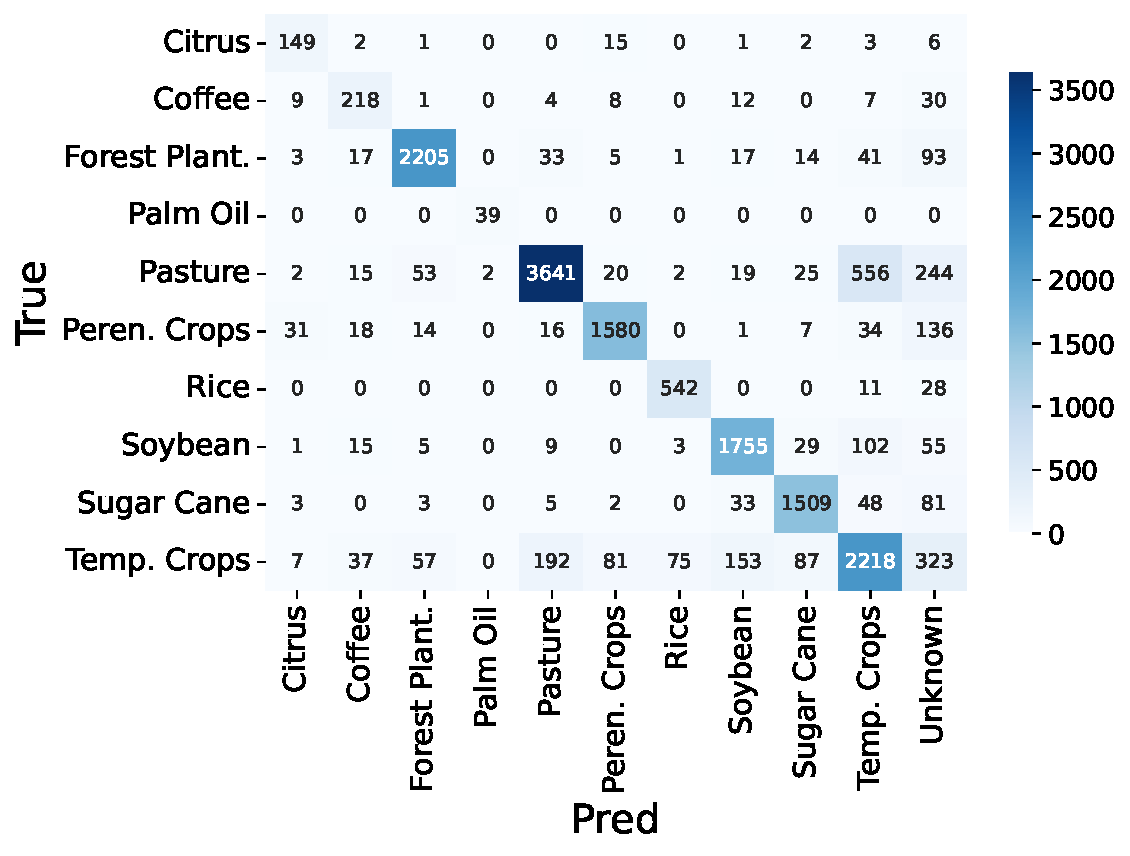
\includegraphics[height=0.45\textheight, width=\textwidth, keepaspectratio]{figures/8_results/brazil-finetuning/BERTPP-70.0-MoCo/class_test_gemmos_matrix.pdf}
                % \caption*{Confusion Matrix}
            \end{figure}
        \end{column}
        \begin{column}{0.52\textwidth}
            \begin{figure}
                \centering
                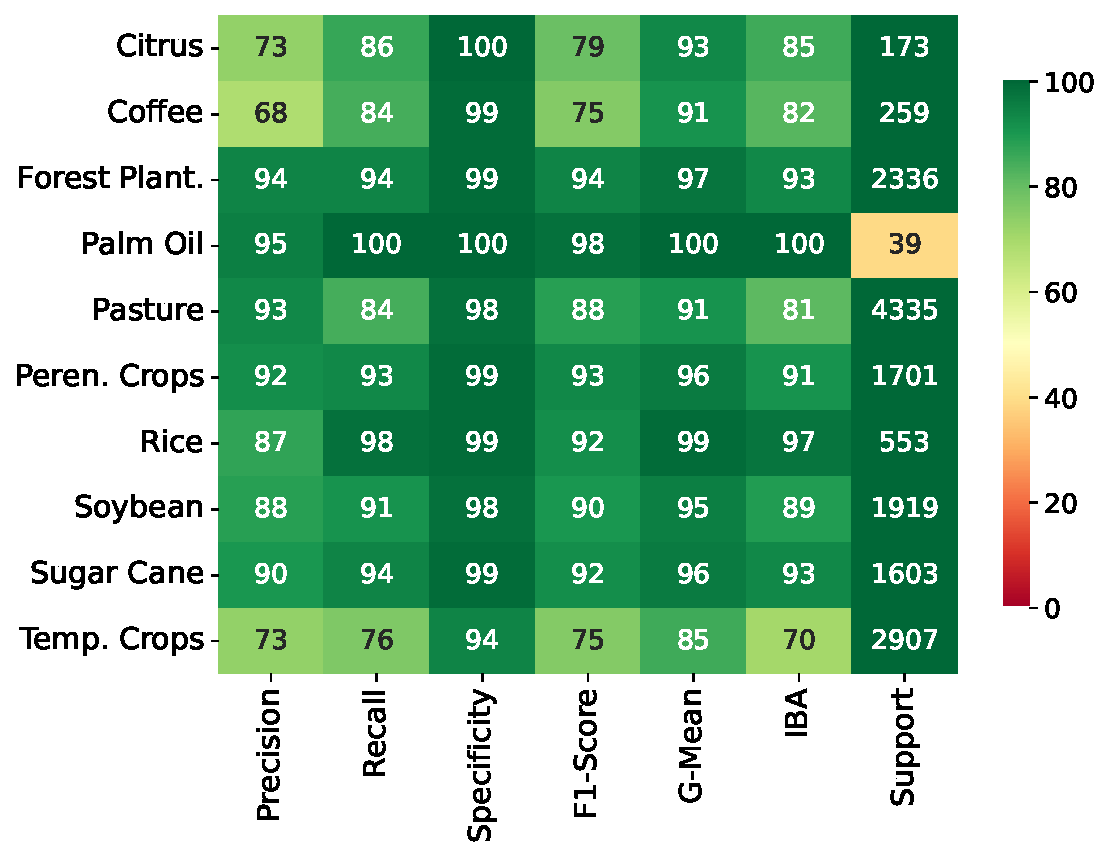
\includegraphics[height=0.45\textheight, width=\textwidth, keepaspectratio]{figures/8_results/brazil-finetuning/BERTPP-70.0-MoCo/class_test_gemmos_report.pdf}
                % \caption*{Confidence Estimation (Log Scale)}
            \end{figure}
        \end{column}
    \end{columns}
\end{frame}

\begin{frame}{Best Setup: Brazil Dataset}
    \begin{block}{SITS-BERT++ (MoCo Pre-training)}
        The proposed ORDER framework achieves a distinct bimodal separation between correct and incorrect predictions for crops like Citrus and Coffee.%, vastly traditional confidence estimators such as ConfidNet and MCP.
    \end{block}
    
    \vspace{0.2cm}
    
    \begin{figure}
        \centering
        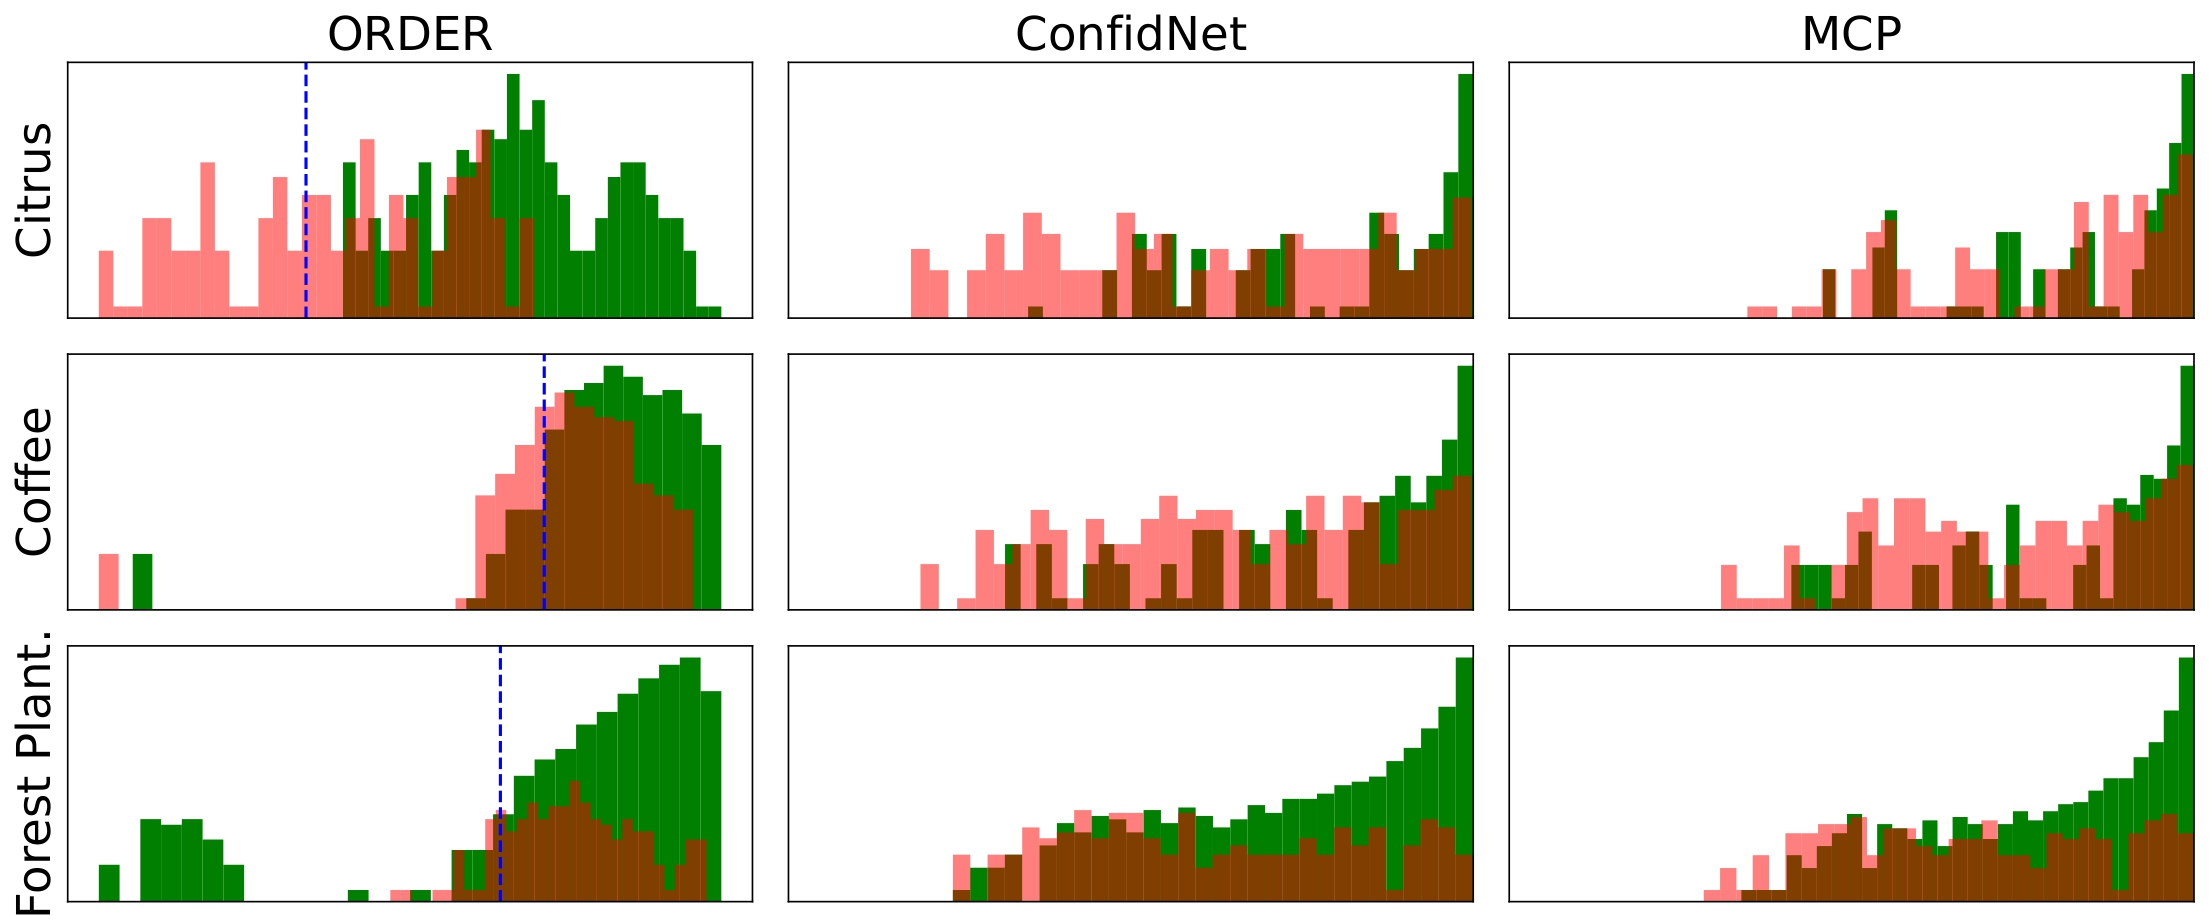
\includegraphics[height=0.41\textheight, width=\textwidth, keepaspectratio]{figures_slides/hist_combined_brasil.jpg}
        % \caption*{Confidence Estimation (Log Scale)}
    \end{figure}

\end{frame}

% --- SLIDE 7: BEST RESULT TEXAS (FIGURAS 65, 66) ---

\begin{frame}{Best Setup: Texas Dataset}
    \begin{block}{SITS-LSTM (FastSiam Pre-training)}
        Transitioning to the Texas dataset, the SITS-LSTM architecture paired with FastSiam pre-training achieves near-perfect classification.%, highlighted by strong diagonal dominance and over 20,000 accurate predictions for Wheat.
    \end{block}
    
    \vspace{0.2cm}
    
    \begin{columns}[T]
        \begin{column}{0.48\textwidth}
            \begin{figure}
                \centering
                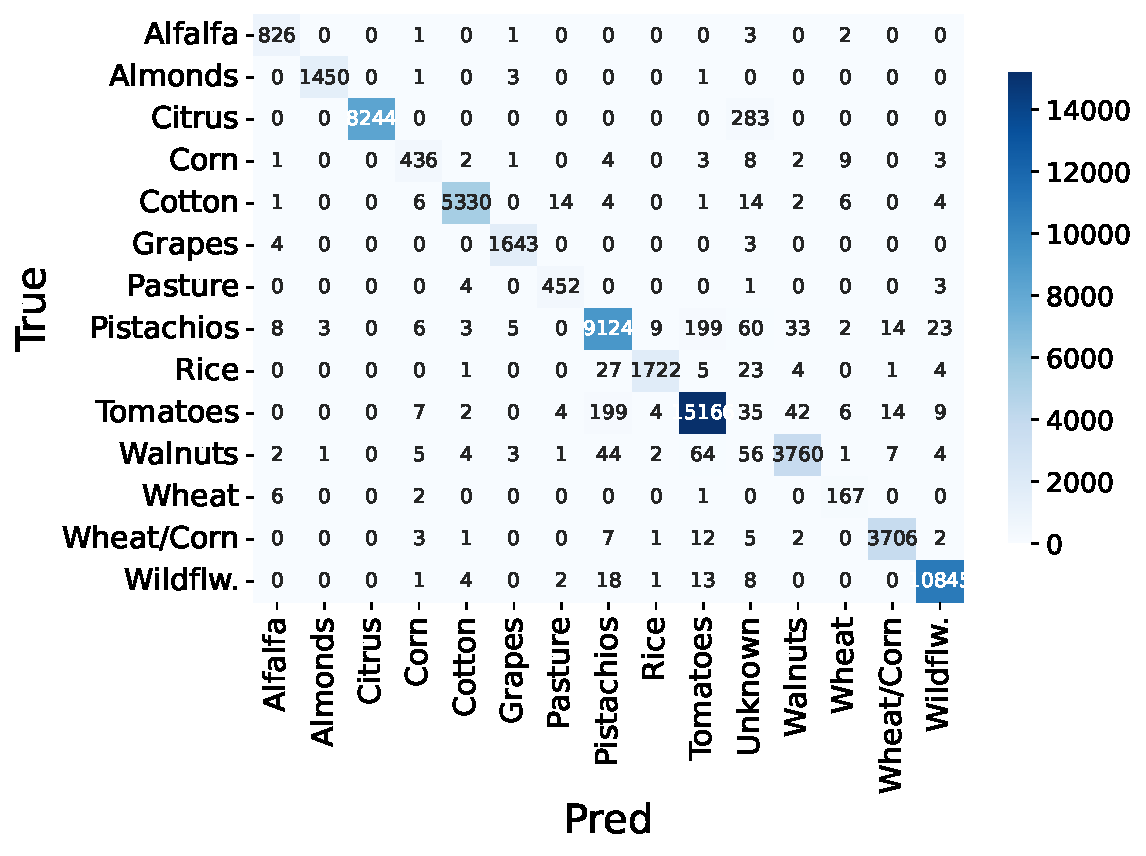
\includegraphics[height=0.45\textheight, width=\textwidth, keepaspectratio]{figures/8_results/california-finetuning/MAMBA-70.0-reconstruct/class_test_gemmos_matrix.pdf}
                % \caption*{Confusion Matrix}
            \end{figure}
        \end{column}
        \begin{column}{0.52\textwidth}
            \begin{figure}
                \centering
                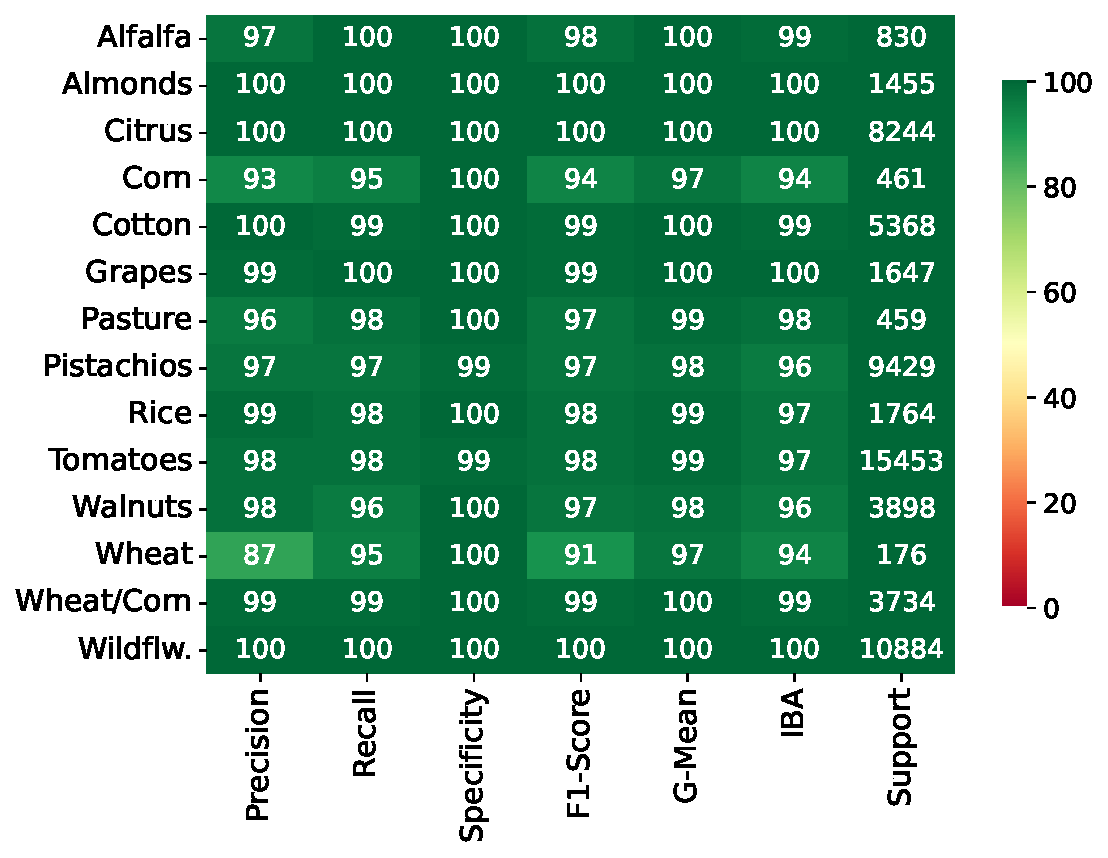
\includegraphics[height=0.45\textheight, width=\textwidth, keepaspectratio]{figures/8_results/california-finetuning/MAMBA-70.0-reconstruct/class_test_gemmos_report.pdf}
                % \caption*{Confidence Estimation (Log Scale)}
            \end{figure}
        \end{column}
    \end{columns}
\end{frame}

\begin{frame}{Best Setup: Texas Dataset}
    \begin{block}{SITS-LSTM (FastSiam Pre-training)}
        Although this exceptionally low error rate challenges standard anomaly visualization, ORDER successfully mitigates the total confidence saturation.% typically observed in baseline methods across classes such as Oats, Cotton, and Corn.
    \end{block}
    
    \vspace{0.2cm}
    
    \begin{figure}
        \centering
        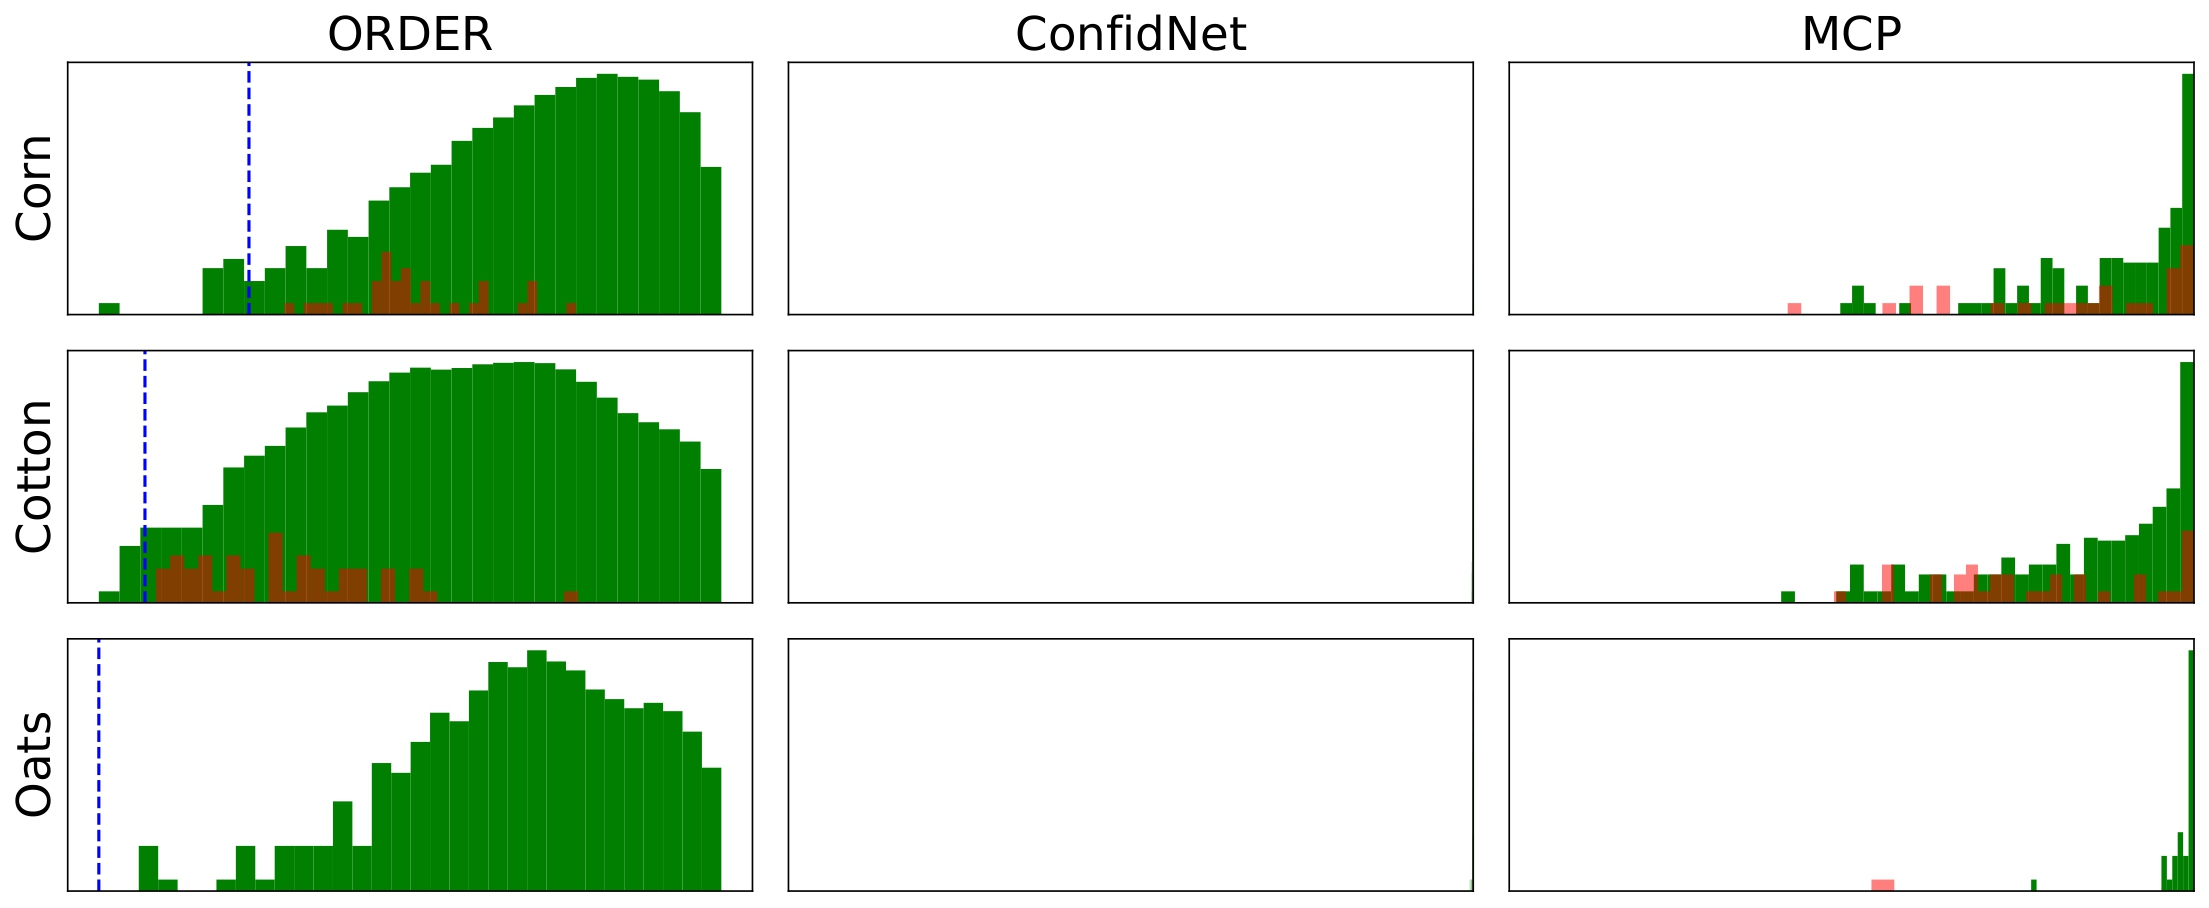
\includegraphics[height=0.41\textheight, width=\textwidth, keepaspectratio]{figures_slides/hist_combined_texas.jpg}
        % \caption*{Confusion Matrix}
    \end{figure}
\end{frame}

% --- SLIDE 8: BEST RESULT CALIFORNIA (FIGURAS 67, 68) ---

\begin{frame}{Best Setup: California Dataset}
    \begin{block}{SITS-Mamba (Masked Modeling Pre-training)}
        For the California dataset, the SITS-Mamba model leverages Masked Modeling pre-training and linear complexity to deliver highly robust performance.%, securing near-perfect predictions for Almonds and Citrus.
    \end{block}
    
    \vspace{0.2cm}
    
    \begin{columns}[T]
        \begin{column}{0.48\textwidth}
            \begin{figure}
                \centering
                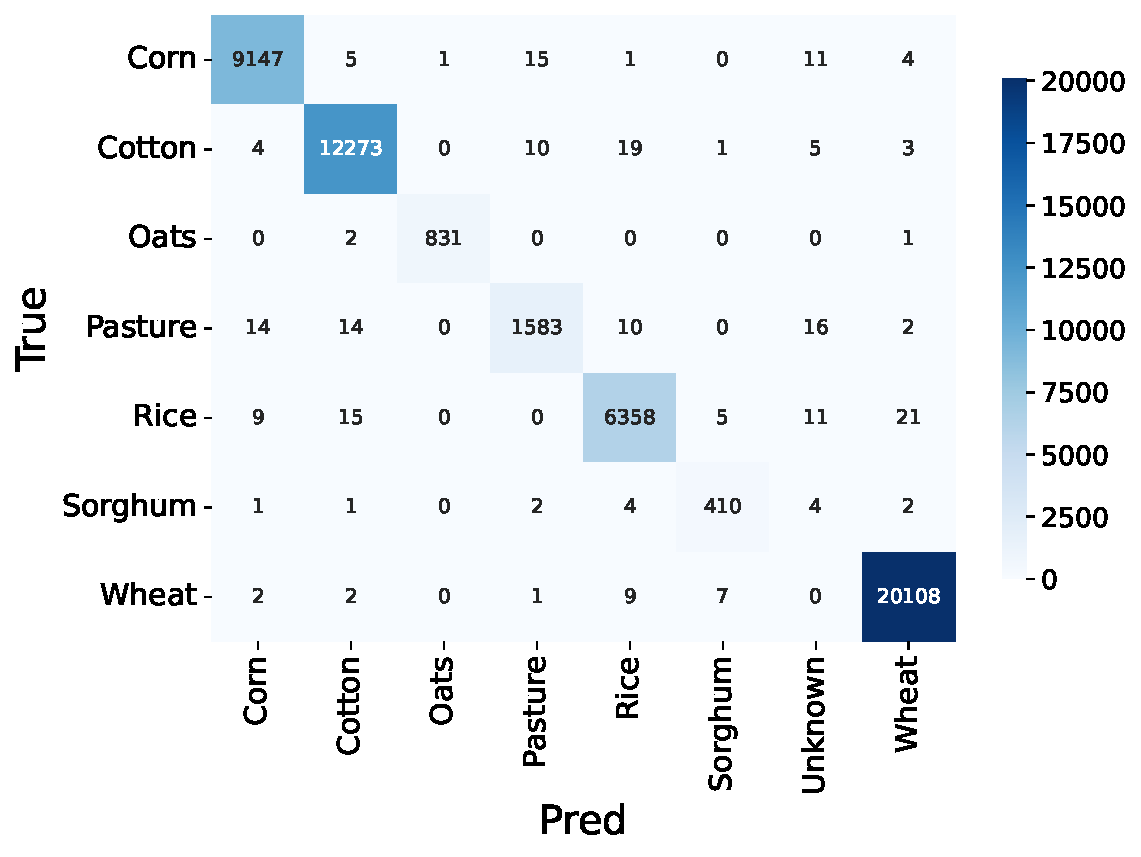
\includegraphics[height=0.45\textheight, width=\textwidth, keepaspectratio]{figures/8_results/texas-finetuning/LSTM-70.0-FastSiam/class_test_gemmos_matrix.pdf}
                % \caption*{Confusion Matrix}
            \end{figure}
        \end{column}
        \begin{column}{0.52\textwidth}
            \begin{figure}
                \centering
                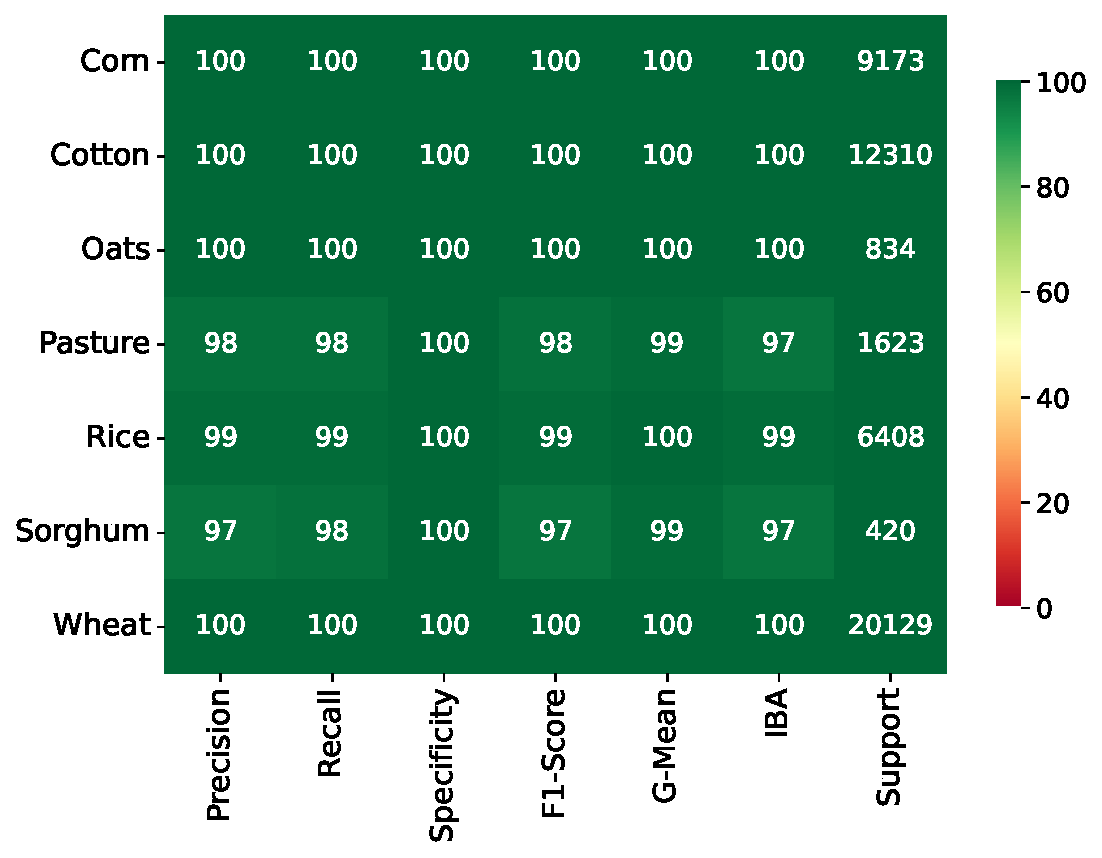
\includegraphics[height=0.45\textheight, width=\textwidth, keepaspectratio]{figures/8_results/texas-finetuning/LSTM-70.0-FastSiam/class_test_gemmos_report.pdf}
                %\caption*{Confidence Estimation (Log Scale)}
            \end{figure}
        \end{column}
    \end{columns}
\end{frame}

\begin{frame}{Best Setup: California Dataset}
    \begin{block}{SITS-Mamba (Masked Modeling Pre-training)}
        Similar to the Texas dataset, the results in California show unsaturated ORDER scores.
    \end{block}
    
    \vspace{0.2cm}
    
    \begin{figure}
        \centering
        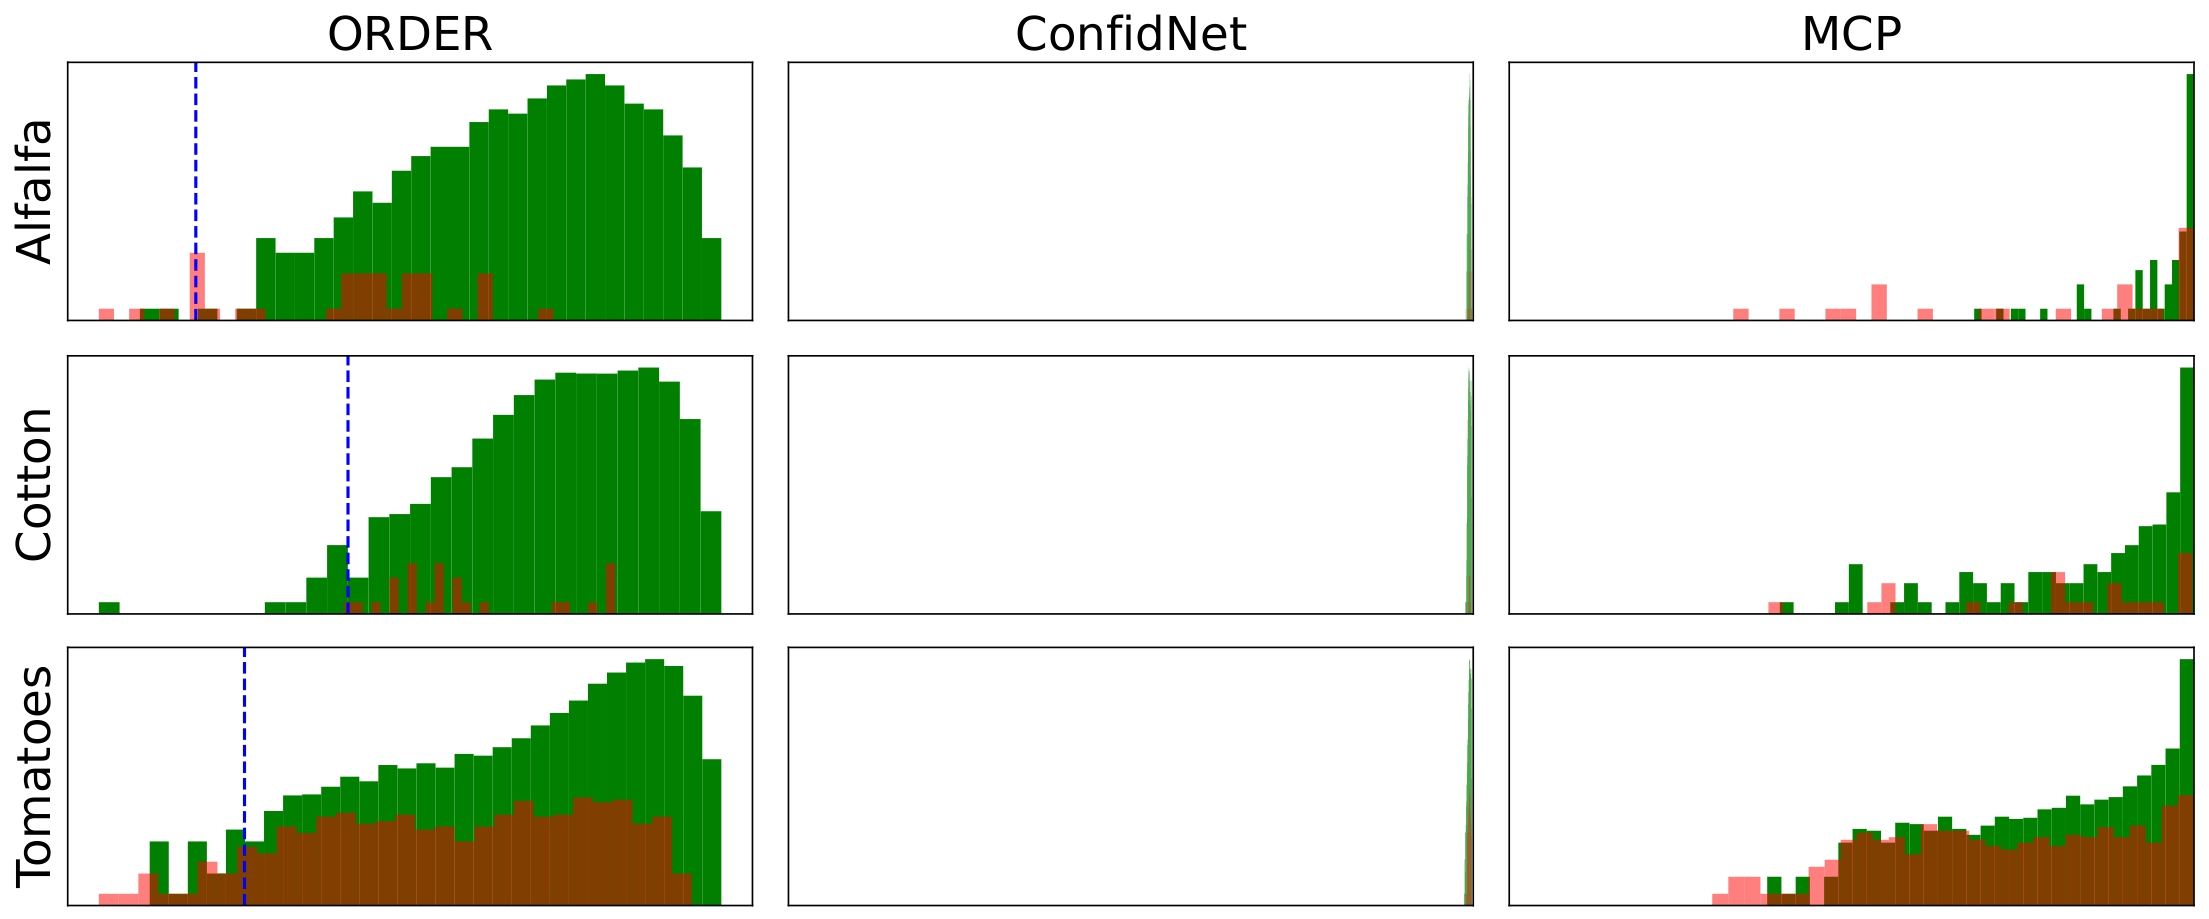
\includegraphics[height=0.41\textheight, width=\textwidth, keepaspectratio]{figures_slides/hist_combined_california.jpg}
        \caption*{Confidence Estimation (Log Scale)}
    \end{figure}
\end{frame}



\section{Conclusion}
\label{sec:08:conclusion}

% --- SLIDE 1: GENERAL SUMMARY ---

\begin{frame}{Concluding Remarks: General Summary}
    \begin{block}{A Data-Centric Lightweight Pipeline}
        This work explored a scalable pipeline for parcel-level crop classification using public labels and Sentinel-2 data. The DCAI filtering strategy allowed the creation of datasets even from noisy public sources.
    \end{block}

    \pause

    \begin{block}{Models \& Reliability}
        \begin{itemize}
            \item Deep Learning models generally showed better performance than Shallow baselines, particularly in complex scenarios like Brazil.
            \item Self-Supervised Learning indicated a positive impact as a regularizer in data-scarce regimes.
            \item The proposed \textbf{ORDER} method demonstrated promising potential in separating correct from incorrect predictions, offering a viable alternative to mitigate model overconfidence.
        \end{itemize}
    \end{block}
\end{frame}

% --- SLIDE 2: RQ1 ---

\begin{frame}{Answering RQ1: Data-Centric AI (DCAI)}
    \begin{block}{Research Question 1}
        To what extent can DCAI strategies - specifically, rigorous filtering of noisy public labels - enable the creation of crop classification datasets and improve the performance of crop classification models?
    \end{block}

    \begin{figure}
        \centering
        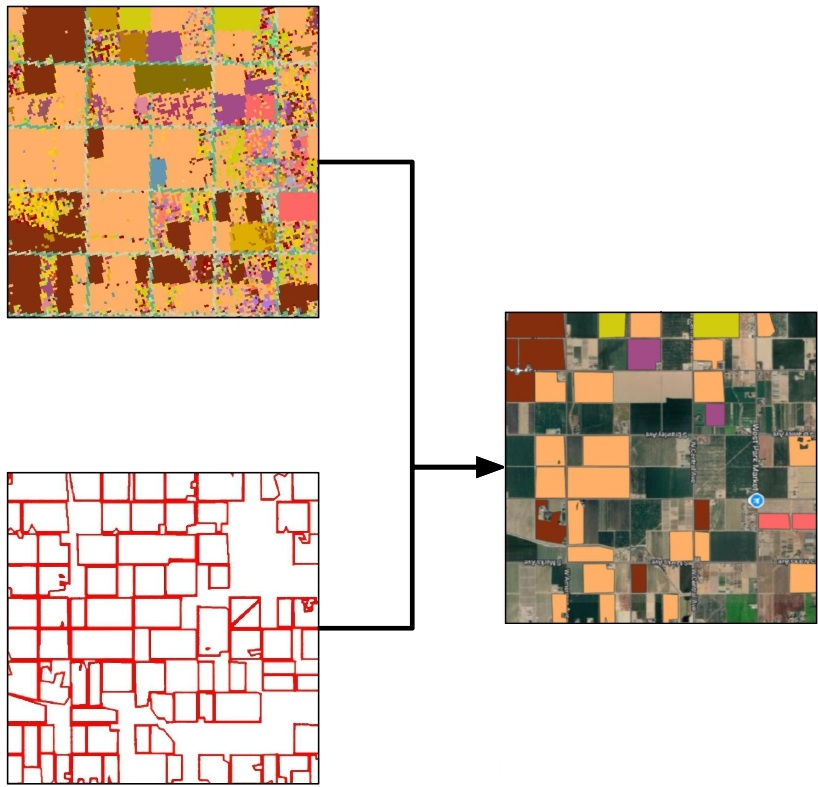
\includegraphics[width=0.4\textwidth, keepaspectratio]{figures_slides/rq1.jpg}
    \end{figure}
\end{frame}

\begin{frame}{Answering RQ1: Data-Centric AI (DCAI)}
    \begin{block}{Research Question 1}
        To what extent can DCAI strategies - specifically, rigorous filtering of noisy public labels - enable the creation of crop classification datasets and improve the performance of crop classification models?
    \end{block}

    \begin{block}{Conclusion}
        \begin{itemize}
            \item The DCAI strategy, combined with public cropland rasters, enables the effective creation of large-scale crop classification datasets.
            \item \textbf{Limitation/Future Work:} To fully isolate and estimate the exact impact of the DCAI performance on downstream models, further studies are necessary, especially focusing on \textbf{actively correcting possible incorrect labels evaluated by the framework}.
        \end{itemize}
    \end{block}
\end{frame}

% --- SLIDE 3: RQ2 ---

\begin{frame}{Answering RQ2: Self-Supervised Learning (SSL)}
    \begin{block}{Research Question 2}
        Do SSL pre-training strategies impact embedding generation and offer a significant advantage over supervised models when labels are scarce? If so, which strategy generates the best embeddings?
    \end{block}

  \begin{figure}
        \centering
        \caption{Few shot (1\%) on Brazil Dataset.}
        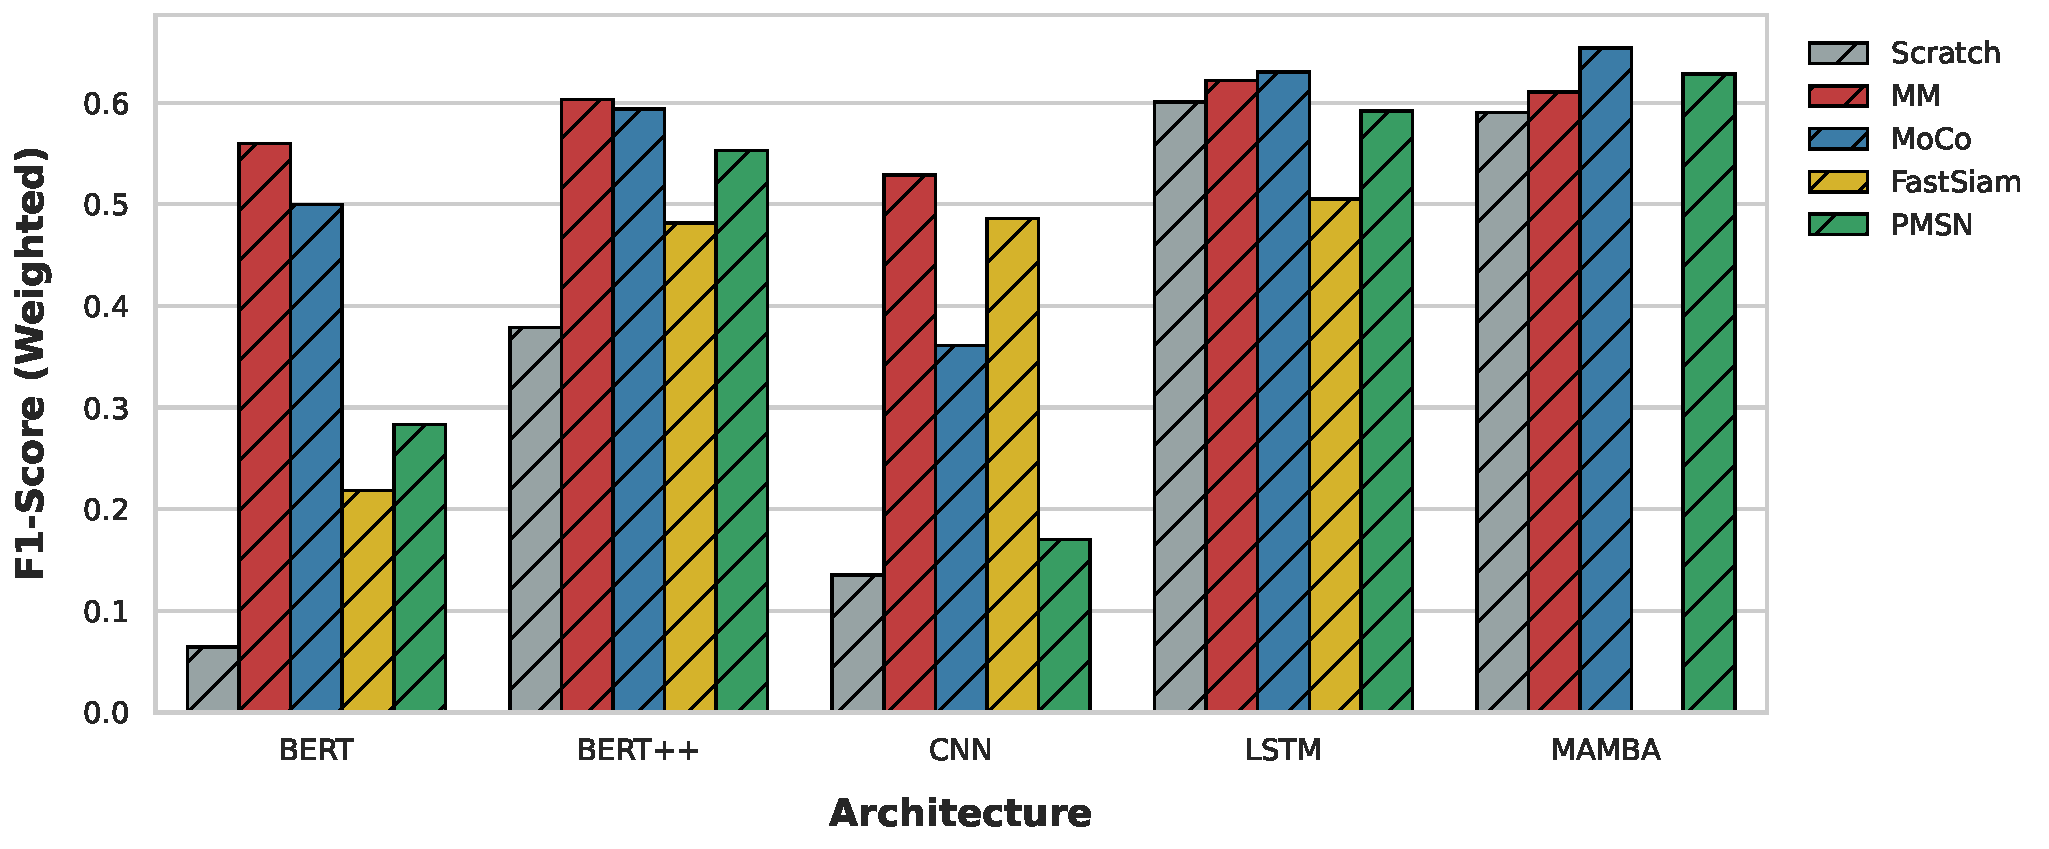
\includegraphics[width=0.8\textwidth, keepaspectratio]{figures/8_results/brazil-finetuning/few_shot_pretraining.pdf}
    \end{figure}
\end{frame}

\begin{frame}{Answering RQ2: Self-Supervised Learning (SSL)}
    \begin{block}{Research Question 2}
        Do SSL pre-training strategies impact embedding generation and offer a significant advantage over supervised models when labels are scarce? If so, which strategy generates the best embeddings?
    \end{block}

    \begin{block}{Conclusion}
        \begin{itemize}
            \item SSL pre-training appears to be a highly effective option for improving classification metrics in label-scarce scenarios (e.g., 1\% and 0.1\% regimes).
            \item Among the evaluated strategies, \textbf{MoCo} stood out, generating consistent metrics in both fine-tuning and direct embedding evaluation (KNN), without presenting severe representation collapse across the experiments.
        \end{itemize}
    \end{block}
\end{frame}

% --- SLIDE 4: RQ3 ---

\begin{frame}{Answering RQ3: Lightweight Pipeline \& Models}
    \begin{block}{Research Question 3}
        Is it possible to build a lightweight pipeline that achieves satisfactory performance for crop classification that can be run without expensive hardware? If so, which models are most suitable?
    \end{block}

  \begin{figure}
        \centering
        %\caption{Few shot (1\%) on Brazil Dataset.}
        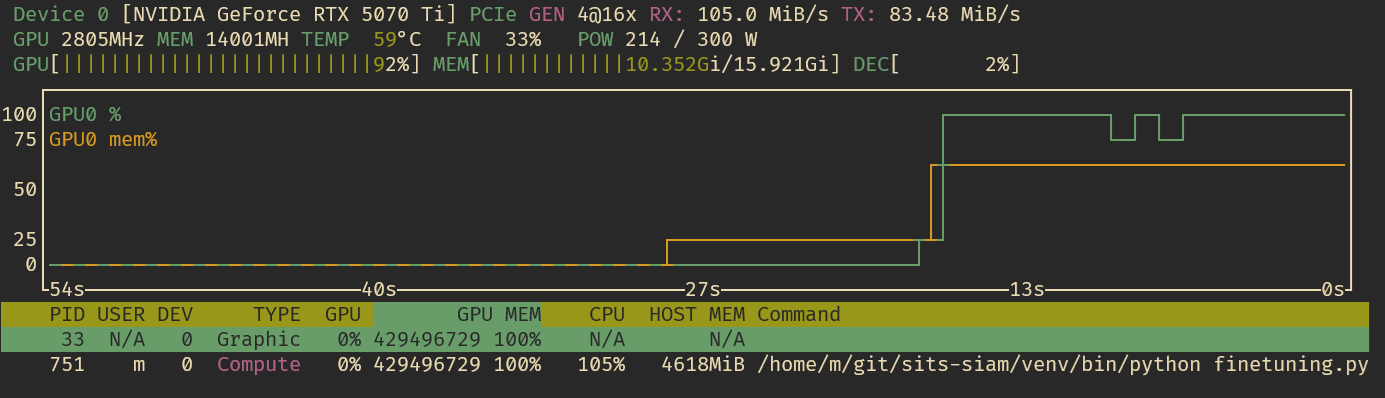
\includegraphics[width=1\textwidth, keepaspectratio]{figures_slides/rq3.png}
    \end{figure}
\end{frame}


\begin{frame}{Answering RQ3: Lightweight Pipeline \& Models}
    \begin{block}{Research Question 3}
        Is it possible to build a lightweight pipeline that achieves satisfactory performance for crop classification that can be run without expensive hardware? If so, which models are most suitable?
    \end{block}

    \begin{block}{Conclusion}
        \begin{itemize}
            \item Yes, the results suggest such a pipeline is feasible. The proposed SITS download method shifts most processing costs to the cloud (GEE), enabling the use of modest local hardware.
            \item \textbf{Suitable Models:} \textbf{SITS-BERT++} yielded slightly higher overall metrics, whereas \textbf{SITS-Mamba} provided a highly balanced trade-off due to its linear processing memory costs, making both strong candidates. All models can be fine-tuned with a modest Nvidia RTX 5070 Ti 16GB.
        \end{itemize}
    \end{block}
\end{frame}

% --- SLIDE 5: RQ4 ---

\begin{frame}{Answering RQ4: Public Sensors Applicability}
    \begin{block}{Research Question 4}
        Is it possible to achieve satisfactory performance for crop classification using only public sensors?
    \end{block}

    \pause

    \begin{block}{Conclusion}
        \begin{itemize}
            \item The experiments indicate that it is indeed possible to generate strong ranking and classification metrics relying exclusively on public missions (such as Sentinel-2).
            \item \textbf{Limitation/Future Work:} To confirm the relative efficiency of this approach, further comparative studies testing these models against private, high-resolution commercial sensors are recommended.
        \end{itemize}
    \end{block}
\end{frame}

% --- SLIDE 6: RQ5 ---

\begin{frame}{Answering RQ5: Anomaly Detection (ORDER)}
    \begin{block}{Research Question 5}
        Is it possible to improve confidence estimation or detect model anomalies through generative models on embeddings, surpassing established baselines such as ConfidNet?
    \end{block}

      \begin{figure}
        \centering
        \caption{Traditional Regime (70\%) on Brazil Dataset, SITS-BERT++ with MoCo.}
        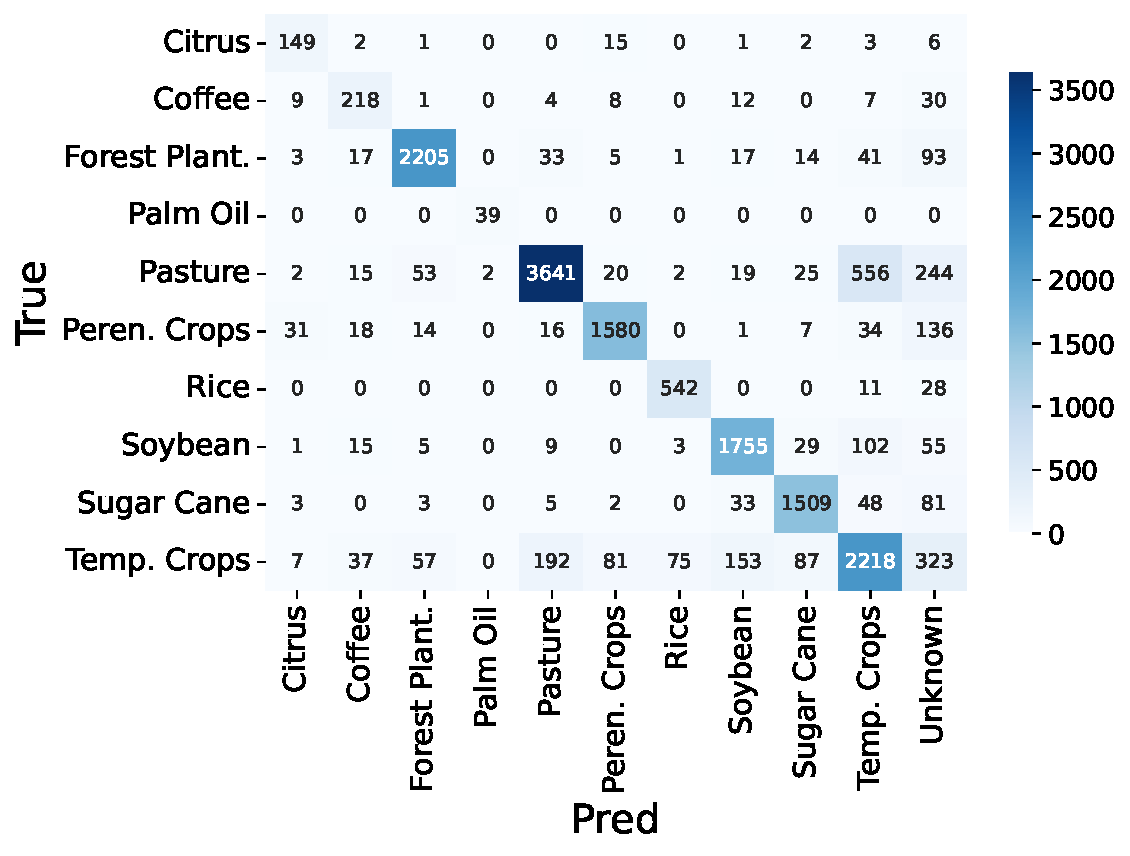
\includegraphics[width=0.4\textwidth, keepaspectratio]{figures/8_results/brazil-finetuning/BERTPP-70.0-MoCo/class_test_gemmos_matrix.pdf}
    \end{figure}
\end{frame}

\begin{frame}{Answering RQ5: Anomaly Detection (ORDER)}
    \begin{block}{Research Question 5}
        Is it possible to improve confidence estimation or detect model anomalies through generative models on embeddings, surpassing established baselines such as ConfidNet?
    \end{block}

    \begin{block}{Conclusion}
        \begin{itemize}
            \item Detecting anomalies during prediction using embedding analysis methods like \textbf{ORDER} proved to be a viable strategy.
            \item \textbf{ORDER} generated a visually clearer bimodal differentiation between correct and incorrect predictions compared to the ConfidNet baseline and the standard Maximum Class Probability (MCP).
            \item While formal confidence ranking was not fully explored, the well-behaved prediction scores suggest it is a promising avenue for future work.
        \end{itemize}
    \end{block}
\end{frame}

\section{Other Contributions}

\begin{frame}{Contributions}
\begin{itemize}
  \item \textbf{(Conference)} \textbf{DA SILVA, Mateus Pinto}; SCHAEFER, Mariana A. R.; OLIVEIRA, Hugo N.; REIS, Julio C. S.; NUNES, Ian M.; DOS SANTOS, Jefersson A. Learning Visual Patterns in Remote Sensing: An Overview of Agricultural Applications. In: 2024 37th SIBGRAPI Conference on Graphics, Patterns and Images (SIBGRAPI). IEEE, 2024. p. 1–6.
  \item \textbf{(Journal)} \textbf{DA SILVA, Mateus Pinto}; CORREA, Sabrina P. L. P.; SCHAEFER, Mariana A. R.; REIS, Julio C. S.; NUNES, Ian M.; DOS SANTOS, Jefersson A.; OLIVEIRA, Hugo N. Advancing Agricultural Remote Sensing: A Comprehensive Review of Deep Supervised and Self-Supervised Learning for Crop Monitoring. Computers \& Graphics, 2025. DOI: 10.1016/j.cag.2025.104434.
\end{itemize}
\end{frame}

\begin{frame}{Contributions}
\begin{itemize}
    \item \textbf{(Journal)} \textbf{DA SILVA, Mateus Pinto}; VIEIRA, Lucas; DE SANTANA, Cleverton T. C.; NUNES, Ian M.; DOS SANTOS, Jefersson A.; OLIVEIRA, Hugo N. A Lightweight Pipeline for Crop Time-Series Parcel Classification via Self-Supervision. IEEE Geoscience and Remote Sensing Letters, 2025, p. 1–1. DOI: 10.1109/LGRS.2025.3589176.
    \item \textbf{(Conference)} DE OLIVEIRA, João Vitor S.; VIEIRA, Danilo F.; \textbf{DA SILVA, Mateus P.}; FERNANDES, Daniel L.; RIBEIRO, Marcos H. F.; OLIVEIRA, Hugo N. Strategies for Deep Learning in Volumetric Medical Imaging: A Survey. 2025 38th SIBGRAPI Conference on Graphics, Patterns and Images (SIBGRAPI), p. 1–6, 2025.
\end{itemize}
\end{frame}

\begin{frame}{Contributions}
\begin{itemize}
    \item \textbf{(Conference)} ALCANTARA, André N.; \textbf{SILVA, Mateus P.}; OLIVEIRA, Hugo N.; REIS, Julio C. S. Assessing the Potential of Large Language Models (LLMs) for the Automatic Generation of Solutions for Programming Exercises. In: ANAIS ESTENDIDOS DO XXXI SIMPÓSIO BRASILEIRO DE SISTEMAS MULTIMÍDIA E WEB (WEBMEDIA 2025) — V CONCURSO DE TRABALHOS DE INICIAÇÃO CIENTÍFICA (CTIC 2025). Sociedade Brasileira de Computação (SBC), 2025. Rio de Janeiro, Brasil.
    \item \textbf{(Bachelor Thesis)} PEREIRA, Lara Fernandes; CORRÊA, Sabrina P. L. P. (Co-Supervisor); \textbf{DA SILVA, Mateus Pinto (Co-Supervisor)}; OLIVEIRA, Hugo Neves (Supervisor). Benchmarking Super-Resolution Models for Remote Sensing in Agricultural Contexts. Undergraduate Thesis (Bachelor's Degree in Computer Science) — Universidade Federal de Viçosa, Viçosa, 2025.
\end{itemize}
\end{frame}

\begin{frame}{Contributions}
\begin{itemize}
    \item \textbf{(Bachelor Thesis)} SOUZA, Bárbara Cristina Fonseca de; CORRÊA, Sabrina P. L. P. (Co-Supervisor); \textbf{DA SILVA, Mateus Pinto (Co-Supervisor)}; OLIVEIRA, Hugo Neves (Supervisor). Open Set Crop Classification Using Deep and Self-Supervised Learning Approaches. Undergraduate Thesis (Bachelor's Degree in Computer Science) — Universidade Federal de Viçosa, Viçosa, 2025.
     \item \textbf{(Journal)} \textbf{DA SILVA, Mateus P.}; NUNES, Ian M.; DOS SANTOS, Jefersson A.; OLIVEIRA, Hugo N. ORDER - Crop Mapping Anomaly Detection using Generative Models. International Journal of Remote Sensing, Submitted.
\end{itemize}
\end{frame}

\begin{frame}{Contributions}
\begin{itemize}
    \item \textbf{(Journal)} CORREA, S. P. L. P.; REIS, M. S.; \textbf{SILVA, M. P.}; DOS SANTOS, J. A.; OLIVEIRA, J. C.; KÖRKING, T. S.; DOS SANTOS, A. P.; DUTRA, L. V. Rethinking Reference Data Quality: The Role of Mixed Pixels in Remote Sensing Classification. International Journal of Remote Sensing, Submitted.
\end{itemize}
\end{frame}



\begin{frame}{Code Contribution: AgriGEE.lite}
    \begin{block}{Democratizing Agricultural SITS}
        To facilitate reproducibility and help other researchers bypass the steep learning curve of Google Earth Engine, we packaged our lightweight methodology into an open-source Python library.
    \end{block}

    \begin{block}{Features of AgriGEE.lite (Available on PyPI)}
        \begin{itemize}
            \item Parallel wrapper for GEE handling asynchronous requests.
            \item Automated calculation of vegetation/water indices (NDVI, EVI2, NDWI, etc.) directly on the server side.
            \item Built-in cloud masking and spatial aggregation statistics for various public sensors.
        \end{itemize}
    \end{block}
\end{frame}

\begin{frame}
    % --- Logos das Instituições Financiadoras ---
    \begin{center}
        % Ajuste o 'height' para o tamanho ideal e o nome dos arquivos das imagens
        
\includegraphics[height=1.2cm]{logos_institutos/logo_ibge.png} \hspace{0.5cm}
        
\includegraphics[height=1.2cm]{logos_institutos/logo_mavilab.png} \hspace{0.5cm}
        
\includegraphics[height=1.2cm]{logos_institutos/logo_patreo.png} \hspace{0.5cm}
        
\includegraphics[height=1.2cm]{logos_institutos/logo_serrapilheira.png}
    \end{center}
    
    \vspace{0.5cm} % Espaço entre os logos e o "Thank You!"
    
    % --- Agradecimento e Dados ---
    \begin{center}
        \LARGE{\textbf{Thank You!}} \\
        \vspace{0.8cm}
        \large{Mateus Pinto da Silva} \\
        \vspace{0.2cm}
        \normalsize{\textit{Universidade Federal de Viçosa (UFV)}} \\
        \vspace{0.8cm}
        \normalsize{\textbf{Questions?}}
    \end{center}
    
    \vfill
    
    \begin{flushleft}
        \tiny{Contact: mateus.p.silva@ufv.br \\
        Registration Code: EF3489}
    \end{flushleft}
\end{frame}

\end{document}